\documentclass[a4paper,11pt]{article}
\usepackage{../../../Template/zemplate}
\usepackage{float}

\includeGlossario

\docTitle{Norme di Progetto}
\docVersion{4.0.0}
\docCreationDate{\frmdata{03}{12}{2016}}
\docLastUpdateDate{\frmdata{10}{07}{2017}}
\docStatus{Approvato}
\docEditors{Jordan Gottardo \\& Giulia Petenazzi \\& Leonardo Brutesco}
\docVerificators{Giovanni Prete}
\docApprovers{Marco Pasqualini}
\docUse{Interno}
\docDestination{\Tullio \\ & \Cardin \\ & \zephyrus}
\docJournal{
4.0.0 & \frmdata{10}{07}{2017} & Marco Pasqualini & \responsabile & Approvazione \\
3.1.0 & \frmdata{06}{07}{2017} & Giovanni Prete & \verificatore & Verifica documento \\
3.0.2 & \frmdata{05}{07}{2017} & Leonardo Brutesco & \analista & Aggiunta sezione per la consegna \\
3.0.1 & \frmdata{26}{06}{2017} & Giulia Petenazzi & \analista & Correzioni e modifche minori al processo di sviluppo \\
3.0.0 & \frmdata{08}{04}{2017} & Giovanni Prete & \responsabile & Approvazione \\
2.1.0 & \frmdata{03}{04}{2017} & Giovanni Damo & \verificatore & Verifica documento \\		
2.0.6 & \frmdata{03}{04}{2017} & Jordan Gottardo & \amministratore & Aggiunte norme per i manuali utente e manutentore\\
2.0.5 & \frmdata{01}{04}{2017} & Giulia Petenazzi & \amministratore & Aggiunte norme di codifica per eseguire import ed export\\
2.0.4 & \frmdata{25}{03}{2017} & Jordan Gottardo & \amministratore & Approfondite sezioni di progettazione ad alto livello e di dettaglio\\
2.0.3 & \frmdata{19}{03}{2017} & Jordan Gottardo & \amministratore & Aggiunta procedura configurazione Webstorm\\
2.0.2 & \frmdata{18}{03}{2017} & Leonardo Brutesco & \amministratore & Aggiunta procedura glossario nei manuali, ampliate norme sullo stile codifica, aggiunti comandi nell'appendice, approfondite norme progettazione, corretta sezione 2.2.5.3\\	
2.0.1 & \frmdata{15}{03}{2017} & Leonardo Brutesco & \amministratore & Aggiunte procedure per configurazione VirtualBox e FileZilla\\
2.0.0 & \frmdata{04}{03}{2017} & Giovanni Damo & \responsabile & Approvazione \\
1.3.0 & \frmdata{03}{03}{2017} & Jordan Gottardo & \verificatore & Verifica documento \\		
1.2.1 & \frmdata{03}{03}{2017} & Marco Pasqualini & \analista & Corretta descrizione WebStorm \\
1.2.0 & \frmdata{02}{03}{2017} & Jordan Gottardo & \verificatore & Verifica documento \\	
1.1.5 & \frmdata{02}{03}{2017} & Marco Pasqualini & \analista & Aggiunto diagramma procedura chiusura ticket, aggiunti WebStorm, JSDoc e Babel agli strumenti del processo di sviluppo \\
1.1.4 & \frmdata{02}{03}{2017} & Marco Pasqualini & \analista & Aggiunta procedura di rinvio dei task e sezione per condivisione in apprendimento \\
1.1.3 & \frmdata{02}{03}{2017} & Marco Pasqualini & \analista & Aggiunte procedure per il calcolo delle metriche \\
1.1.2 & \frmdata{01}{03}{2017} & Giulia Petenazzi & \analista & Creazione tabelle riassuntive metriche-strumenti-procedure \\
1.1.1 & \frmdata{28}{02}{2017} & Marco Pasqualini & \analista & Aggiunte metriche al processo di verifica. Correzione errori ortografici \\
1.1.0 & \frmdata{26}{02}{2017} & Jordan Gottardo & \verificatore & Verifica documento \\
1.0.10 & \frmdata{25}{02}{2017} & Marco Pasqualini & \analista & Aggiunta classificazione test e correzione errori nel processo di sviluppo \\
1.0.9 & \frmdata{23}{02}{2017} & Marco Pasqualini & \analista & Aggiunte procedure per installazione macchina virtuale e segnalazione richieste \\
1.0.8 & \frmdata{21}{02}{2017} &Giulia Petenazzi & \analista & Ampliata sezione gestione delle infrastrutture, aggiunti strumenti Node.js, npm, VirtualBox e integrazioni Slack \\
1.0.7 & \frmdata{19}{02}{2017} & Marco Pasqualini & \analista & Ampliate procedure utilizzo Trender \\
1.0.6 & \frmdata{17}{02}{2017} & Marco Pasqualini & \analista & Aggiunti strumenti ESLint e JSMeter agli strumenti di analisi statica, Karma, Jasmine e Istanbul agli strumenti di analisi dinamica \\
1.0.5 & \frmdata{15}{02}{2017} & Marco Pasqualini & \analista & Creato processo di gestione della configurazione. Spostate sezioni Repository, Versionamento, Git, GitHub e relative procedure in gestione della configurazione \\
1.0.4 & \frmdata{15}{02}{2017} & Marco Pasqualini & \analista & Aggiunta appendice per comandi \LaTeX \\
1.0.3 & \frmdata{13}{02}{2017} & Marco Pasqualini & \analista & Inserite procedure per Astah, calcolo Indice Gulpease e aggiunti termini al glossario \\
1.0.2 & \frmdata{12}{02}{2017} & Marco Pasqualini & \analista & Inserite procedure di consegna, di creazione dei documenti e di utilizzo Slack. Aggiornate sezioni \LaTeX{} e Apprendimento \\
1.0.1 & \frmdata{29}{01}{2017} & Marco Pasqualini & \analista & Messi a glossario i termini solo la prima volta che compaiono in ogni sezione del documento \\
1.0.0 & \frmdata{23}{12}{2016} & Giulia Petenazzi & \responsabile & Approvazione \\
0.2.0 & \frmdata{20}{12}{2016} & Leonardo Brutesco & \verificatore & Verifica documento \\
0.1.1 & \frmdata{20}{12}{2016} & Giovanni Prete & \analista & Correzione errori \\
0.1.0 & \frmdata{17}{12}{2016} & Leonardo Brutesco & \verificatore & Verifica documento \\
0.0.10 & \frmdata{17}{12}{2016} & Giovanni Prete & \analista & Correzioni e aggiornamento diagrammi \\
0.0.9 & \frmdata{16}{12}{2016} & Giovanni Damo & \analista & Correzioni sezione processi primari \\
0.0.8 & \frmdata{13}{12}{2016} & Giovanni Prete & \analista & Correzioni sezione processi di organizzativi \\
0.0.7 & \frmdata{09}{12}{2016} & Giovanni Damo & \analista & Correzioni sezione processi  di supporto\\
0.0.6 & \frmdata{07}{12}{2016} & Giovanni Prete & \analista & Aggiunte descrizioni attività e processi \\
0.0.5 & \frmdata{07}{12}{2016} & Giovanni Damo & \analista & Terminata sezione processi di supporto \\
0.0.4 & \frmdata{05}{12}{2016} & Giovanni Damo & \analista & Terminata sezione processi organizzativi \\
0.0.3 & \frmdata{05}{12}{2016} & Giovanni Prete & \analista & Terminata sezione processi primari \\
0.0.2 & \frmdata{04}{12}{2016} & Giovanni Prete & \analista & Terminata introduzione \\
0.0.1 & \frmdata{03}{12}{2016} & Giovanni Prete & \analista & Creazione template e indice \\
}

\usepackage{multirow}

\begin{document}
\section{Introduzione}
    \subsection{Scopo del documento}
    Questo documento definisce le norme che i membri del \glo{Gruppo}{gruppo} \zephyrus{} si impegnano a rispettare per un corretto svolgimento del progetto \progetto{}. Ogni componente del gruppo è tenuto a leggere e rispettare quanto scritto al fine di:
    \begin{itemize}
        \item garantire uniformità nel materiale prodotto;
        \item favorire la cooperazione tra i membri del gruppo;
        \item raggiungere il miglior rapporto tra efficacia ed efficienza.
    \end{itemize}
    Il presente documento definisce le norme inerenti a:
    \begin{itemize}
        \item comunicazioni interne ed esterne al gruppo;
        \item stesura dei documenti e convenzioni tipografiche;
        \item stesura del codice;
        \item modalità di lavoro durante il \glo{Ciclo di vita}{ciclo di vita} del progetto;
        \item organizzazione dell'ambiente di lavoro e di sviluppo.
    \end{itemize}
    Ogni membro del gruppo sarà informato di eventuali modifiche alle norme esistenti o aggiunta di nuove norme.

    \subsection{Scopo del prodotto}
        \introScopo

    \subsection{Glossario}
        \introGlossario

    \subsection{Riferimenti}
        \subsubsection{Riferimenti normativi}
        \begin{itemize}
            \item \textbf{standard \glo{ISO}{ISO}-8601:}\\ \url{https://en.wikipedia.org/wiki/ISO_8601}; \label{sec:iso8601}
            \item \textbf{standard ISO/\glo{IEC}{IEC} 12207:}\\ \url{https://en.wikipedia.org/wiki/ISO/IEC_12207};
            \item \textbf{specifica \glo{UML}{UML} 2.0:}\\ \url{http://www.omg.org/spec/UML/2.0/}.
        \end{itemize}

        \subsubsection{Riferimenti informativi} \label{sec:riferimenti}
        \begin{itemize}
            \item \textbf{standard AS/NZS ISO/IEC 12207:1997:}\\ \url{http://www.math.unipd.it/~tullio/IS-1/2009/Approfondimenti/ISO_12207-1995.pdf}; \label{sec:isoiec}
            \item \textbf{\glo{Capitolato}{capitolato}:}\\ \url{http://www.math.unipd.it/~tulXlio/IS-1/2016/Progetto/C3.pdf};
            \item \textbf{utilizzo di \glo{Teamwork}{Teamwork}:}\\ \url{http://support.teamwork.com/projects/start/getting-started};
            \item \textbf{utilizzo di \glo{Git}{Git}}:\\ \url{https://git-scm.com/doc};
            \item \textbf{utilizzo di \glo{GitHub}{GitHub}}:\\ \url{https://guides.github.com/};
            \item \textbf{utilizzo di \glo{Astah}{Astah}:}\\ \url{http://astah.net/tutorials};
            \item \textbf{utilizzo di \glo{Slack}{Slack}:}\\ \url{https://get.slack.help/hc/en-us}.
        \end{itemize}

\section{Processi primari}
    \subsection{Fornitura}
        \subsubsection{Scopo}
        Lo scopo del processo di fornitura è di determinare le procedure e le risorse necessarie allo svolgimento del progetto. Le attività di cui si compone sono:
        \begin{itemize}
            \item studio di fattibilità;
            \item contrattazione;
            \item collaudo.
        \end{itemize}
        La corretta implementazione del processo deve:
        \begin{itemize}
            \item decidere il progetto da svolgere;
            \item fissare gli obiettivi per la contrattazione.
        \end{itemize}
        \subsubsection{Studio di fattibilità}
            \paragraph{Scopo}
            Individuare gli aspetti fondamentali dei progetti proposti, tramite lo studio dei \glo{Capitolato}{capitolati} ed il confronto tra i membri del \glo{Gruppo}{gruppo}.
            \paragraph{Discussione e scelta del capitolato}
            Il \responsabilediprogetto{} ha il compito di organizzare gli incontri del gruppo necessari ad analizzare i capitolati proposti.
            \paragraph{Struttura studio di fattibilità}
            Il documento creato dagli \analisti{} per ogni capitolato deve rispettare i seguenti punti:
            \begin{itemize}
                \item \textbf{descrizione:} descrizione del prodotto richiesto dal capitolato;
                \item \textbf{dominio applicativo:} ambito di utilizzo del prodotto;
                \item \textbf{dominio tecnologico:} tecnologie richieste per lo sviluppo del progetto;
                \item \textbf{criticità:} individuazione di punti critici e possibili problematiche che potrebbero sorgere durante lo svolgimento del progetto;
                \item \textbf{valutazione finale:} considerazioni finali sulla scelta di accettare o meno il capitolato preso in esame.
            \end{itemize}
        \subsubsection{Contrattazione}
            \paragraph{Scopo}
            Presentare una proposta in risposta al capitolato del proponente.
            \paragraph{Preparazione della proposta}
            Il gruppo deve redigere e consegnare i seguenti documenti:
            \begin{itemize}
                \item \ndp;
                \item \sdf;
                \item \adr;
                \item \pdp;
                \item \pdq.
            \end{itemize}
            Verrà inoltre fornita in allegato la \ldp{} del gruppo. Si veda la sezione \ref{sec:classDoc} per maggiori informazioni sulla gestione dei documenti.
        \subsubsection{Consegna}
	        \paragraph{Scopo}
	        Preparare il materiale richiesto per la \revacc.
	        \paragraph{Preparazione della consegna}
	        Deve essere preparato un supporto ottico (CD/DVD) contente:
		    \begin{itemize}
		    	\item la \ldp{} del gruppo per la \revacc;
		    	\item le versioni finali di tutti i documenti;
		    	\item il prodotto finale realizzato comprensivo di:
			    	\begin{itemize}
			    		\item codice sorgente;
			    		\item eventuali unità di compilazione e installazione;
			    		\item istruzioni per l'uso.
			    	\end{itemize}
		    \end{itemize}
	        Il \responsabilediprogetto{} ha il compito di contattare il committente per richiedere un appuntamento per consegnare il supporto preparato.
	        \paragraph{Consegna}
	        Il \responsabilediprogetto{} deve contattare il proponente per accordarsi sulle modalità di consegna del prodotto finale.
		\subsubsection{Procedure}
			\paragraph{Primo contatto con il proponente}
			Il primo contatto con il proponente da parte del gruppo \zephyrus{} deve essere effettuato da parte del \responsabilediprogetto{}. L'oggetto del messaggio deve contenere la sigla del progetto; il messaggio deve essere realizzato secondo la seguente struttura:
			\bigskip
				\begin{verbatim}
				Spett.le Nome Azienda, 
				alla cortese attenzione del CEO/Responsabile Nome Cognome;
				
				... corpo del messaggio ...
				
				Vi ringraziamo e speriamo di poterci incontrare presto di persona.
				
				Cordiali saluti,
				Zephyrus.
				\end{verbatim}
			\paragraph{Consegna materiale per revisione di avanzamento}
			La consegna del materiale prodotto deve rispettare i vincoli temporali descritti al seguente indirizzo:
			\begin{center}
				\url{http://www.math.unipd.it/~tullio/IS-1/2016/}
			\end{center}
			L'invio del materiale deve essere gestito nel seguente modo:
			\begin{enumerate}
				\item creare una cartella compressa contenente tutti e soli i documenti inerenti la consegna in formato pdf. Il nome della cartella sarà: \texttt{Zephyrus-XX.zip} dove al posto di XX sarà presente il codice identificativo della revisione di avanzamento;
				\item caricarla sullo spazio web del gruppo, disponibile al seguente indirizzo:
				\begin{center}
% 	\href{https://s311.altervista.org/lf.pl?sid=e085c1d3474a6fb0a08d56cafc9e60e3https://s311.altervista.org/lf.pl?sid=e085c1d3474a6fb0a08d56cafc9e60e3}{Altervista Zephyrus}
					\href{http://zephyrusar.altervista.org/}{Altervista Zephyrus}
				\end{center}
			\item contattare con l'email del gruppo, il committente all'indirizzo \url{tullio.vardanega@math.unipd.it} e allegare il link al file precedentemente caricato su Altervista.
			\end{enumerate}
    \subsection{Sviluppo}
        \subsubsection{Scopo}
	        Il processo di sviluppo contiene le attività necessarie a produrre il prodotto software richiesto. In accordo con lo standard \glo{ISO}{ISO}/\glo{IEC}{IEC} (\ref{sec:isoiec}), preso come riferimento, si è deciso di istanziare le seguenti attività:
        \begin{itemize}
            \item analisi dei requisiti;
            \item progettazione;
            \item codifica.
        \end{itemize}
        La corretta implementazione del processo deve:
        \begin{itemize}
            \item fissare gli obiettivi di sviluppo;
            \item fissare i vincoli tecnologici;
            \item realizzare un prodotto finale che soddisfi i test di accettazione e che sia conforme alle richieste del proponente.
        \end{itemize}
        \subsubsection{Analisi dei requisiti}
            \paragraph{Scopo}
            Individuare i requisiti del progetto tramite lo studio del capitolato ed incontri con il proponente. Individuare i test di sistema. Il risultato deve essere presentato nel documento formale \adr{} che deve contenere la lista dei casi d'uso e dei requisti.
            \paragraph{Classificazione dei casi d'uso}
            I casi d'uso individuati devono essere classificati secondo la seguente notazione:
            \begin{center}
            UC[Codice padre].[Codice identificativo]
            \end{center}
            dove:
            \begin{itemize}
                \item \textbf{codice padre:} indica il codice numerico in forma gerarchica del caso d'uso da cui deriva, viene omesso se non identificabile;
                \item \textbf{codice identificativo:} indica il codice numerico del caso d'uso.
            \end{itemize}
            Per ogni caso d'uso bisogna indicare:
            \begin{itemize}
                \item \textbf{titolo:} titolo riassuntivo dell'operazione che il caso d'uso modella;
                \item \textbf{attori:} elenco attori coinvolti;
                \item \textbf{descrizione:} concisa e meno ambigua possibile;
                \item \textbf{pre-condizione:} condizioni sempre vere riferite allo stato del sistema che abilitano lo svolgimento del caso d'uso;
                \item \textbf{post-condizione:} condizioni sempre vere riferite allo stato del sistema dopo lo svolgimento del caso d'uso;
                \item \textbf{scenario principali:} ordine con cui vengono eseguiti i casi d'uso figli;
                \item \textbf{scenari alternativi:} possibili scenari alternativi del caso d'uso;
                \item \textbf{estensioni:} spiegazione di tutte le estensioni, se presenti;
                \item \textbf{inclusioni:} spiegazione di tutte le inclusioni, se presenti;
                \item \textbf{generalizzazioni:} spiegazione di tutte le generalizzazioni, se presenti.
            \end{itemize}

            \paragraph{Classificazione dei requisiti}
            I requisiti individuati devono essere classificati secondo la seguente notazione:
            \begin{center}
            R[Importanza][Tipologia][Codice]
            \end{center}
            dove:
            \begin{itemize}
                \item \textbf{importanza:} può assumere questi valori:
                \begin{itemize}
                    \item \textbf{O:} indica un requisito obbligatorio;
                    \item \textbf{D:} indica un requisito desiderabile;
                    \item \textbf{F:} indica un requisito opzionale (facoltativo).
                \end{itemize}
                \item \textbf{tipologia:} può assumere questi valori:
                \begin{itemize}
                    \item \textbf{F:} indica un requisito funzionale;
                    \item \textbf{Q:} indica un requisito di qualità;
                    \item \textbf{P:} indica un requisito prestazionale;
                    \item \textbf{V:} indica un requisito di vincolo.
                \end{itemize}
                \item \textbf{codice:} codice numerico che identifica il requisito, deve essere univoco ed indicato in forma gerarchica, da sinistra a destra, nella notazione X.Y.Z.
            \end{itemize}
            Per ogni requisito bisogna inoltre indicare:
            \begin{itemize}
                \item \textbf{descrizione:} concisa e meno ambigua possibile;
                \item \textbf{fonte:} l'origine dei requisiti deve essere una delle seguenti:
                \begin{itemize}
                    \item \textbf{capitolato:} derivato direttamente dal testo del capitolato;
                    \item \textbf{interno:} deriva da discussioni interne al gruppo;
                    \item \textbf{verbale:} deriva da un verbale steso in seguito ad un incontro con il proponente. Deve essere indicato il nome del verbale a cui si riferisce;
                    \item \textbf{casi d'uso:} deriva da uno o più casi d'uso. Deve essere indicato il codice identificativo dei casi d'uso a cui si riferisce.
                \end{itemize}
            \end{itemize}
            \paragraph{Diagrammi UML} \label{sec:astahStyle}
                I diagrammi \glo{UML}{UML} devono essere realizzati seguendo lo standard UML versione 2. \\
                Per facilitare la lettura dei diagrammi si devono seguire le seguenti convenzioni generali:
                \begin{itemize}
                % considerare di separare per tipo di diagramma es: casi d'uso e diagrammi delle classi
                    \item gli elementi devono essere il più possibile omogenei tra loro per dimensione;
                    \item gli elementi devono essere allineati tra loro, sia orizzontalmente che verticalmente, quando possibile;
                    \item i margini di spazio tra gli elementi di un gruppo devono rimanere invariati in gruppi analoghi se si hanno le stesse tipologie di elementi;
                    \item i collegamenti in uscita da un singolo elemento devono essere ad angolo retto invece che diretti.
                \end{itemize}
            \subsubsection{Progettazione ad alto livello}
                \paragraph{Scopo}
                Definire la struttura di alto livello del software e identificare le sue componenti. Definire le interfacce esterne ed interne. Individuare i test di integrazione. Il risultato deve essere presentato nel documento formale \st.
                \paragraph{Specifica tecnica}
                \subparagraph{Diagrami UML}
                Devono essere forniti i seguenti diagrammi:
                \begin{itemize}
                    \item \textbf{diagrammi di classe:} hanno lo scopo di descrivere entità con le loro caratteristiche e relazioni, pertanto vengono definiti attributi, metodi e relazioni. tra di esse. Nella progettazione ad alto livello non è necessario che questi diagrammi siano particolarmente dettagliati;
                    \item \textbf{diagrammi dei \glo{Package}{package}:} hanno lo scopo di rappresentare la struttura interna del progetto software modellato in termini dei suoi componenti principali. Questo tipo di diagramma viene utilizzato per evidenziare i package e le relazioni tra i componenti interni ed esterni che siano;
                    \item \textbf{diagrammi di attività:} hanno lo scopo di definire le attività da svolgere per realizzare una certa funzionalità. Vengono dunque usati per mostrare come determinate interazioni tra componenti realizzino una funzionalità che si intende rendere disponibile.
                    %\item diagrammi di sequenza. %TODO da lasciare o no?
                \end{itemize}
	            Viene introdotta una notazione che utilizza i colori per distinguere la provenienza delle componenti dell'applicazione:
	            \begin{itemize}
	            	\item giallo: \glo{Componente}{componente} da implementare;
	            	\item rosso: componente offerta da \riskapp;
	            	\item verde: componente importata da terze parti.
	            \end{itemize}
            	%
                \subparagraph{Design pattern}
                Per migliorare la comprensibilità delle scelte progettuali e della progettazione stessa devono essere forniti i \glo{Design pattern}{design pattern} utilizzati secondo la seguente struttura:
	            \begin{itemize}
	            	\item descrizione testuale;
	            	\item descrizione grafica;
	            	\item motivazione e descrizione dell'utilizzo all'interno del progetto.
	            \end{itemize}
            
	            \subparagraph{Classificazione dei componenti}
	            I componenti vengono identificati univocamente da una descrizione nella forma:
	            \begin{center}
					[NomeProdotto]::[NomeComponente]
	            \end{center}
				dove:
				\begin{itemize}
					\item \textbf{NomeProdotto:} è il nome del prodotto software che i \progettisti{} hanno individuato;
					\item \textbf{NomeComponente:} rappresenta il nome assegnato al componente dai \progettisti.
				\end{itemize}
				Inoltre, ogni componente ha associato un codice univoco nella forma:
				\begin{center}
				[X][Y]
				\end{center}
				dove:
				\begin{itemize}
					\item \textbf{X:} è l'iniziale del nome del prodotto; 
					\item \textbf{Y:} è un numero intero incrementale.
				\end{itemize}
			
				\subparagraph{Definizione delle classi}
				I \progettisti{} devono fornire la seguente definizione per ogni componente:
				\begin{itemize}
					\item nome;
					\item struttura del componente;
					\item descrizione;
					\item classi contenute.
				\end{itemize}
                \subparagraph{Tracciamento delle componenti}
                Tutti i requisiti devono essere riferiti al componente che li soddisfa per poter verificare che ogni requisito sia soddisfatto.  \\
                Si veda la sezione \ref{sec:trender} in cui viene descritto lo strumento utilizzato per il tracciamento e la sezione \ref{sec:traccComp} per le procedure di gestione dei componenti.
                \subparagraph{Test di integrazione}\label{sec:testInt}
                Devono essere definite le classi di verifica necessarie a garantire che tutte le componenti del sistema funzionino correttamente. \\
                Si veda la sezione \ref{sec:trender} in cui viene descritto lo strumento utilizzato per il tracciamento e la sezione \ref{sec:traccTint} per le procedure di gestione dei test di integrazione.
                
            \subsubsection{Progettazione a basso livello}
                \paragraph{Scopo}
                Definire la struttura di tutte le componenti e suddivederle in unità che possanno essere realizzate, compilate e testate singolarmente. Individuare i test delle unità. Il risultato deve essere presentato nel documento formale \ddp.
                \paragraph{Definizione di prodotto}
                \subparagraph{Diagrammi UML}
                Devono essere forniti i seguenti diagrammi:
                \begin{itemize}
                    \item \textbf{diagrammi di classe:}  hanno lo scopo di descrivere entità con le loro caratteristiche e relazioni, pertanto vengono definiti attributi, metodi e relazioni. tra di esse. Nella progettazione di dettaglio è necessario che questi diagrammi siano particolarmente dettagliati;
                    \item \textbf{diagrammi di attività:} hanno lo scopo di definire le attività da svolgere per realizzare una certa funzionalità. Vengono dunque usati per mostrare come determinate interazioni tra componenti realizzino una funzionalità che si intende rendere disponibile;
                    \item \textbf{diagrammi di sequenza:} hanno lo scopo di descrivere le relazioni che intercorrono, in termini di messaggi, tra attori, oggetti ed entità del sistema software rappresentato.
                \end{itemize}
	            Viene introdotta una notazione che utilizza i colori per distinguere la provenienza delle componenti dell'applicazione:
	            \begin{itemize}
	            	\item giallo: componente da implementare;
	            	\item rosso: componente offerta da \riskapp;
	            	\item verde: componente importati da terze parti.
	            \end{itemize}
	            \subparagraph{Design pattern}
	            Per migliorare la comprensibilità delle scelte progettuali e della progettazione stessa devono essere forniti i \glo{Design pattern}{design pattern} utilizzati secondo la seguente struttura:
	            \begin{itemize}
	            	\item descrizione testuale;
	            	\item descrizione grafica;
	            	\item motivazione e descrizione dell'utilizzo all'interno del progetto.
	            \end{itemize}
	            \subparagraph{Classificazione delle classi}
	             Le classi vengono identificate univocamente da una descrizione nella forma:
	            \begin{center}
					[NomeProdotto]::[NomeComponente]::[NomeClasse]
	            \end{center}
	            dove:
	            \begin{itemize}
	            	\item \textbf{NomeProdotto:} è il nome del prodotto software che i \progettisti{} hanno individuato;
	            	\item \textbf{NomeComponente:} rappresenta il nome assegnato al componente dai \progettisti;
	            	\item \textbf{NomeClasse:} rappresenta il nome che è stato dato dai \progettisti{} alla classe individuata.
	            \end{itemize}
	            
                \subparagraph{Definizione delle classi}
                I \progettisti{} devono fornire la seguente definizione per ogni classe:
                \begin{itemize}
                	\item nome;
                	\item visibilità;
                	\item attributi;
                	\item metodi;
                	\item descrizione generica che ne spieghi lo scopo e che definisca le funzionalità.
                \end{itemize}
                \subparagraph{Tracciamento delle classi}
                Tutti i requisiti devono essere tracciati alle classi associate per poter verificare che ogni classe soddisfi almeno un requisito. Si veda le sezione \ref{sec:trender} in cui viene descritto lo strumento utilizzato per il tracciamento.
                \subparagraph{Test di unità}\label{sec:testUnit}
                Devono essere definiti dei test di unità necessari a garantire che tutte le componenti del sistema funzionino correttamente. \\
                Si veda le sezione \ref{sec:trender} in cui viene descritto lo strumento utilizzato per il tracciamento e la sezione \ref{sec:traccTuni} per le procedure di gestione dei test d'unità.
                
            \subsubsection{Codifica e test}
                \paragraph{Scopo}
                Sviluppare le unità ed i test individuati durante la progettazione. Il risultato finale deve essere il codice sorgente del prodotto da realizzare e dei test necessari.
                
                \paragraph{Stile di codifica} \label{codeStyle}
                Al fine di produrre codice uniforme, leggibile e manutenibile è richiesto che vengano rispettate le seguenti convenzioni:
                \begin{itemize}
                    \item i nomi utilizzati devono essere chiari, descrittivi rispetto alla loro funzione e in inglese;
                    \item evitare nomi troppo simili tra loro che possano creare difficoltà nella comprensione del codice;
                    \item deve essere presente almeno un breve commento descrittivo per ogni classe e metodo;
                    \item i commenti devono essere scritti in lingua italiana senza utilizzare abbreviazioni o altre ambiguità;
                    \item le modifiche al codice devono sempre riflettersi sui relativi commenti;
                    \item evitare commenti superflui, inappropriati o scurrili;
                    \item ogni file deve presentare un'intestazione con le seguenti informazioni:
                        \begin{itemize}
                        	\item nome e cognome dell'autore;
                            \item percorso e nome del file;
                            \item data di creazione;
							\item data ultima modifica;
                        \end{itemize}
                \end{itemize}
	            Il codice deve seguire le linee guida reperibili all'indirizzo:
	            \begin{center} \label{sec:stileCodifica}
	            	\url{https://github.com/airbnb/javascript/tree/master/react}
	            \end{center}
            	Ulteriori convenzioni adottate sono:
            	\begin{itemize}
            		\item i nomi delle classi devono rispettare lo stile PascalCase;
            		\item i seguenti nomi devono rispettare lo stile CamelCase:
            			\begin{itemize}
            				\item metodi;
            				\item variabili;
            				\item nomi dei file;
            			\end{itemize}
            		\item tutti i campi dati e le variabili devono essere dichiarati pubblici;
            		\item lo stile css deve essere definito \textit{Inline} per ogni componente e deve essere inserito all'interno del costruttore dello stesso;
            		\item per esportare classi, funzioni, oggetti o tipi primitivi da un file (o modulo) si utilizza l'istruzione \hicode{export} di \jsv{}:
            			\begin{itemize}
            				\item per esportare  più valori per file come ad esepio oggetti, variabili, funzioni (può essere usato anche più volte nello stesso modulo). Esempio: \hicode{export let objectEmpty = \{\};}
            				\item per esportare un componente intero (l'istruzione va inserita necessariamente in fondo al file) \hicode{export \{ NomeClasse \}; }
            				%\item \textbf{export default:} per esportare classi, oggetti, funzioni; può essere %usato solo una volta per file;  Esempio \hicode{export default function() \{\} }
            			\end{itemize}
            		\item per importare funzioni, oggetti o tipi primitivi da un file (o modulo) si utilizza l'istruzione \hicode{import} di \jsv{}:
            			\begin{itemize}
            				\item per importare un singolo oggetto o funzione. Esempio: \\ \hicode{import * as stubStrings from '../stubs/stubStrings-spec';} dove \hicode{stubStrings} è un alias del nome del file che si desidera importare. Poi all'interno del file si utilizzerà nel seguente modo: \hicode{stubStrings.nomeOggetto}
            				\item per importare una intera classe esportata: Esempio: \\ \hicode{import \{ Asset \} from '../../src/DeGeOP/store/process/asset';} Non vanno inserite le estensioni nei nomi dei file.
            			\end{itemize}
            	\end{itemize}
            	
           		\paragraph{Documentazione del codice}
           		Per rendere maggiormente manutenibile il codice, tutti i \programmatori{} devono documentare ogni componente del codice prodotto (metodo o classe) con la notazione JSDoc3.
           		
           		Successivamente verrà generato un sito web contenente il riepilogo di ciascun componente codificato. Quindi è necessario attenersi alle seguenti regole, in modo tale da generare una documentazione uniforme e precisa. \\
           		Ogni componente deve avere i seguenti tag:
           		\begin{itemize}
           			\item \textbf{@author <name>:} dove al posto di \hicode{<name>}, ci sarà il nome e cognome dello sviluppatore che l'ha realizzato. Esempio: \hicode{@auhor Nome Cognome};
           			\item \textbf{@description Creazione: <date>:} dove al posto di \hicode{<date>} ci sarà la data di creazione del componente, nel formato YYYY-MM-GG. Esempio: \hicode{@description Creazione: 2017-03-01};
           			\item \textbf{@description Ultima modifica: <date>:} dove al posto di \hicode{<date>} ci sarà la data dell'utima modifica del componente, nel formato YYYY-MM-GG. Esempio: \hicode{@description Ultima modifica: 2017-03-01};
           			\item \textbf{@description <desc>:} dove al posto di \hicode{<desc>} ci sarà la descrizione concisa del funzionamento e ruolo del componente. Esempio: \hicode{@description Descrizione del funzionamento...}.
           		\end{itemize} 
           		Inoltre, ogni classe deve avere i seguenti \glo{Tag}{tag}:
           		\begin{itemize}
           			\item \textbf{@class <name>:} dove al posto di \hicode{<name>}, ci sarà il nome della classe. Esempio: \hicode{@class NomeClasse};
           			\item \textbf{@memberof <parentNamepath>:} dove al posto di \hicode{<parentNamepath>} ci sarà il percorso del padre della classe. Esempio: \hicode{@memberof app::front-end::nomePadre};
           			\item \textbf{@param <{type}> <name> [<desc>]:} dove al posto di \hicode{<\{type\}>}, \hicode{<name>} e \hicode{<desc>} ci saranno rispettivamente, tipo dell'attributo, nome, breve descrizione del membro della classe. Esempio: \hicode{@param \{string\} s Descrizione di s...}
           			\item \textbf{@constructs <name>:} dove al posto di \hicode{<name>}, ci sarà il nome del costruttore. Esempio: \hicode{@constructs NomeCostruttore}.
           		\end{itemize}
           		Inoltre ogni metodo deve avere i seguenti tag:
           		\begin{itemize}
           			\item \textbf{@memberof <parentNamepath>:} dove al posto di \hicode{<parentNamepath>} ci sarà il nome della classe del metodo. Esempio: \hicode{@memberof NomeClasse};
           			\item \textbf{@param <{type}> <name> [<desc>]:} dove al posto di \hicode{<\{type\}>}, \hicode{<name>} e \hicode{<desc>} ci saranno rispettivamente, tipo del parametro, nome, breve descrizione. Esempio Esempio: \hicode{@param \{number\} n Descrizione di n...};
           			\item \textbf{@return <{type}> <desc>:} dove al posto di \hicode{<\{type\}>} e \hicode{desc} ci saranno rispettivamente, tipo di ritorno del metodo e breve descrizione.
           			Esempio \hicode{@return \{string\} Questo metodo ritorna una stringa}
           		\end{itemize} 
           		I precedenti tag sono i fondamentali richiesti, ma per una maggiore documentazione si rimanda alla sezione \ref{sec:jsdoc}.
           		            	
                \paragraph{Ricorsione}
                La ricorsione va sempre evitata se possibile. Per ogni funzione ricorsiva è necessario fornire una prova di terminazione nei commenti.
                \paragraph{Variabili globali}
                L'uso di variabili globali va sempre evitato se possibile.
				%
				\paragraph{Classificazione dei test}
				I test implementati devono essere classificati secondo la seguente notazione:
				\begin{center}
					T[Tipologia Test][Codice identificativo]
				\end{center}
				dove:
				\begin{itemize}
					\item \textbf{tipologia test:} indica il tipo di test e può assumere i seguenti valori:
					\begin{itemize}
						\item \textbf{U:} per i test di unità (vedi sezione \ref{sec:testUnit});
						\item \textbf{I:} per i test di integrazione (vedi sezione \ref{sec:testInt});
						\item \textbf{S:} per i test di sistema;
					\end{itemize}
					\item \textbf{codice identificativo:} indica il codice numerico del test.
				\end{itemize}
				%
				\subsubsection{Strumenti}
				\paragraph{Astah} \label{sec:astah}
				% 1)descrizione veloce dell'app
				% 2)cosa ci permette di fare
				\glo{Astah}{Astah} è un'applicazione per la creazione di diagrammi UML ed è utilizzata nel corso delle attività di analisi e progettazione. I diagrammi che verranno realizzati sono:
				\begin{itemize}
					\item di sequenza;
					\item di attività;
					\item dei casi d'uso;
					\item delle classi.
				\end{itemize}
				% 3) perche l'abbiamo scelta
				Le principali motivazioni che hanno portato il gruppo alla scelta di questo strumento sono:
				\begin{itemize}
					\item utilizzato in aula dal docente;
					\item versione professional gratuita con la licenza studente;
					\item \glo{Cross-platform}{cross-platform}.
				\end{itemize}
				% 4) indirizzo dove collegarsi
				Indirizzi per il download del programma e della licenza studente:
				\begin{center}
					\url{http://astah.net/download} \\
					\url{http://astah.net/student-license-request}
				\end{center}
				%
				\paragraph{Babel} \label{sec:Babel}
				\glo{Babel}{Babel} è un compilatore \js{} che permette di trasformare in maniera automatica codice scritto con lo standard ES2015 in codice compatibile con la maggior parte dei browser. Il suo utilizzo è necessario poiché, ad oggi, lo standard ES2015 non è pienamente supportato da tutti i browser. Babel può essere integrato facilmente in WebStorm.\\
				Per ulteriori informazioni:
				\begin{center}
					\url{https://babeljs.io/}
				\end{center}
				%
				\paragraph{JSDoc3} \label{sec:jsdoc}
				JSDoc3 è un tool che permette la generazione automatica di documentazione per \glo{JavaScript}{JavaScript}, simile a JavaDoc o PHPDoc. JSDoc3 sfrutta delle annotazioni (es: @author) per documentare il codice direttamente nei file sorgenti. La documentazione finale sarà generata sotto forma di sito web. JSDoc3 scansionerà i file javascript interpretando le annotazioni generando cosi le pagine \glo{HTML}{HTML}. \\
				Questo strumento è utilizzato durante l'attività di codifica e le principali motivazioni che hanno portato il gruppo alla sua scelta sono:
				\begin{itemize}
					\item larga diffusione;
					\item documentazione vasta, professionale e altamente usabile.
				\end{itemize}
				L'indirizzo per la documentazione dello strumento è:
				\begin{center}
					\url{http://usejsdoc.org/index.html}
				\end{center}
				%
				\paragraph{Trender}\label{sec:trender}
				Il gruppo utilizza l'applicazione \glo{Trender}{Trender} per gestire i dati ricavati dall'analisi dei requisiti. Trender è stato sviluppato dal gruppo InfiniTech per il progetto dell'anno 2014/15, utilizza un \glo{Database}{database} \glo{MySQL}{MySQL} per la persistenza dei dati ed è disponibile al seguente indirizzo:
				\begin{center}
					\url{https://github.com/campagna91/Trender}.
				\end{center}
				Le funzionalità offerte da Trender sono:
				\begin{itemize}
					\item tracciamento dei requisiti;
					\item tracciamento dei casi d’uso;
					\item tracciamento dei verbali;
					\item tracciamento degli attori presenti nel sistema;
					\item tracciamento dei \glo{Package}{packages};
					\item tracciamento delle classi;
					\item tracciamento dei test;
					\item tracciamento delle voci del glossario;
					\item possibilità di creare il codice \glo{Latex}{\LaTeX{}} di quanto archiviato nei punti precedenti;
					\item statistiche su: requisiti, casi d'uso, componenti, test.
				\end{itemize}
				Lo spazio di lavoro dedicato al gruppo si trova al seguente indirizzo:
				\begin{center}
					\url{http://zephyrusar.altervista.org/trender/}
				\end{center}
				%
				\paragraph{WebStorm} \label{sec:WebStorm}
				% 1)descrizione veloce dell'app
				\glo{WebStorm}{WebStorm} è un \glo{IDE}{IDE} fornito dall'azienda JetBrains per lo sviluppo di applicazioni e siti web.
				% 2)cosa ci permette di fare
				Questo software permette di supportare lo sviluppatore nella realizzazione di prodotti web. \\
				Tra le principali funzionalità sono presenti:
				\begin{itemize}
					\item assistenza nella codifica dei principali framework web;
					\item auto-completamento per la sintassi di molti linguaggi (es. Javascript, HTML, \glo{CSS}{CSS});
					\item gestione di progetti complessi;
					\item integrazione con i più popolari tool per lo sviluppo web;
					\item integrazione di un sistema di debugging per il codice JavaScript;
					\item compatibilità con sistemi di build automatico.
				\end{itemize}
				% 3) perche l'abbiamo scelta
				Questo strumento è utilizzato durante l'attività di codifica e le principali motivazioni che hanno portato il gruppo alla sua scelta sono:
				\begin{itemize}
					\item strumento completo e professionale;
					\item licenza gratuita per studenti;
					\item integrabilità con strumenti per analisi statica e test;
					\item integrabilità con \glo{GitHub}{GitHub};
					\item cross-platform.
				\end{itemize}
				% 4) indirizzo dove collegarsi
				L' indirizzo per il download è:
				\begin{center}
					\url{https://www.jetbrains.com/webstorm/download/}
				\end{center}
		%
        \subsubsection{Procedure}
        	\paragraph{Configurazione Astah}
        		\begin{itemize}
        			\item \textbf{Rimozione lock file:} per evitare errori dovuti alla condivisione dei file Astah nella cartella Dropbox è necessario disabilitare l'impostazione che blocca il file quando è aperto nel seguente modo:
        				\begin{itemize}
        					\item aprire Astah;
        					\item entrare nella sezione del menù \hicode{Preferences->File};
        					\item rimuovere la spunta su \hicode{Lock file when opening}.
        				\end{itemize}
        			\item \textbf{Qualità immagini esportate:} per impostare la qualità ad almeno 720p, è necessario:	
        				\begin{itemize}
        					\item aprire Astah;
        					\item entrare nella sezione del menù \hicode{Preferences->Image Export};
        					\item settare il campo dati \hicode{Resolution to export diagram" a 200},
        					\item applicare le modifiche e salvare.
        				\end{itemize}
        		\end{itemize}
        		
			\paragraph{Creazione diagrammi UML con Astah}
	        Per la creazione dei diagrammi UML è stata scelta l'applicazione Astah di cui si rimanda alla sezione \ref{sec:astah} per il download e l'installazione. \\
			Dopo aver aperto Astah, un diagramma UML deve essere creato rispettando il seguente ordine:
			\begin{enumerate}
				\item selezionare dal menù \hicode{Diagram} il tipo di diagramma desiderato;
				\item realizzare il diagramma con le convenzioni descritte nella sezione \ref{sec:astahStyle};
				\item salvarlo nella cartella del documento di riferimento all'interno dello spazio Dropbox \hicode{/Diagrammi Astah/}.
			\end{enumerate}
	    \paragraph{Linking elementi all'interno di un diagramma Astah}
	    Per facilitare la consultazione dei diagrammi, soprattutto tra i casi d'uso, Astah mette a disposizione la funzionalità di collegare tra loro dei componenti all'interno di un diagramma. Per poter effettuare un link bisogna seguire i seguenti passi:
	    \begin{enumerate}
	    	\item selezionare un elemento all'interno del diagramma;
	    	\item click destro su quest'ultimo e selezionare la voce \hicode{Hyperlink -> Edit Hyperlink};
	    	\item click su \hicode{Add Model \& Element};
	    	\item selezionare l'elemento che si vuole collegare.
	    \end{enumerate}
	    Per la modifica o la rimozione dei link si segue la stessa procedura fino al punto 2 per poi cliccare su \hicode{benvegn} piuttosto che su \hicode{Delete}.
	    \paragraph{Aggiunta attore su Trender}
	    L'aggiunta di un attore deve rispettare i seguenti passi:
	    \begin{enumerate}
	    	\item login al sito \url{http://zephyrusar.altervista.org/trender/};
		    \item cliccare sulla voce del menu: \hicode{Actors};
			\item cliccare sul tasto \hicode{+} rosso, in basso a destra;
			\item compilare i campi: \hicode{nome attore, descrizione, padre (opzionale)};
	    	\item cliccare sul tasto \hicode{insert}.
	    \end{enumerate}
	    \begin{figure}[H]
	    	\centering
	    	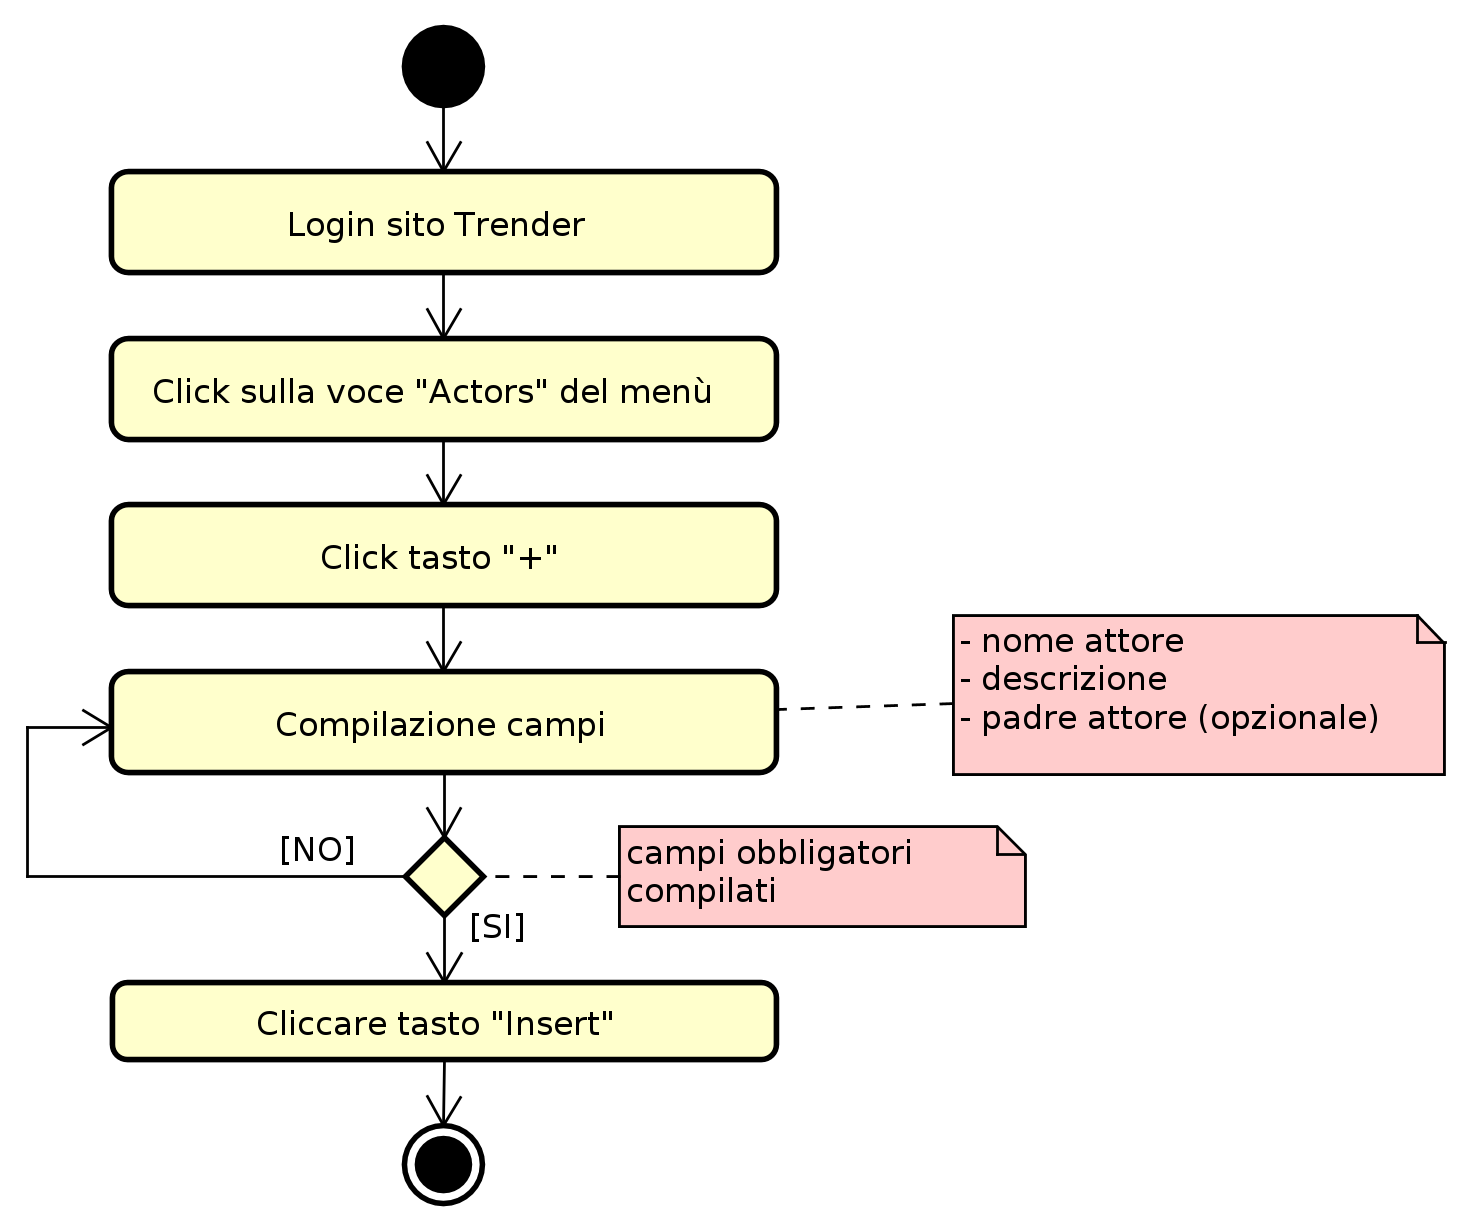
\includegraphics[width=0.7\textwidth]{img/AggiuntaAttore}
	    	\caption{Aggiunta attore.}
	    \end{figure}
	    \paragraph{Modifica ed eliminazione attore su Trender}
	    Questa funzionalità non è stata implementata, pertanto bisogna effettuare la modifica dei campi dati dell'attore o l'eliminazione attraverso l'interfaccia di PhpMyAdmin selezionando la tabella: \texttt{Actors}.
	    
	    \paragraph{Aggiunta use case su Trender}
	    L'aggiunta di uno use case deve rispettare i seguenti passi:
	    \begin{enumerate}
	    	\item login al sito \url{http://zephyrusar.altervista.org/trender/};
	    	\item cliccare sulla voce del menu: \hicode{Usecases};
	    	\item cliccare sul tasto \hicode{+} rosso, in basso a destra;
	    	\item compilare i campi: padre, tipo, titolo, descrizione,  pre-condizione, post-condizione, scenario, estensione, path immagine, didascalia immagine;
	    	\item cliccare sul tasto \hicode{insert}.
	    \end{enumerate}
	    \begin{figure}[H]
	    	\centering
	    	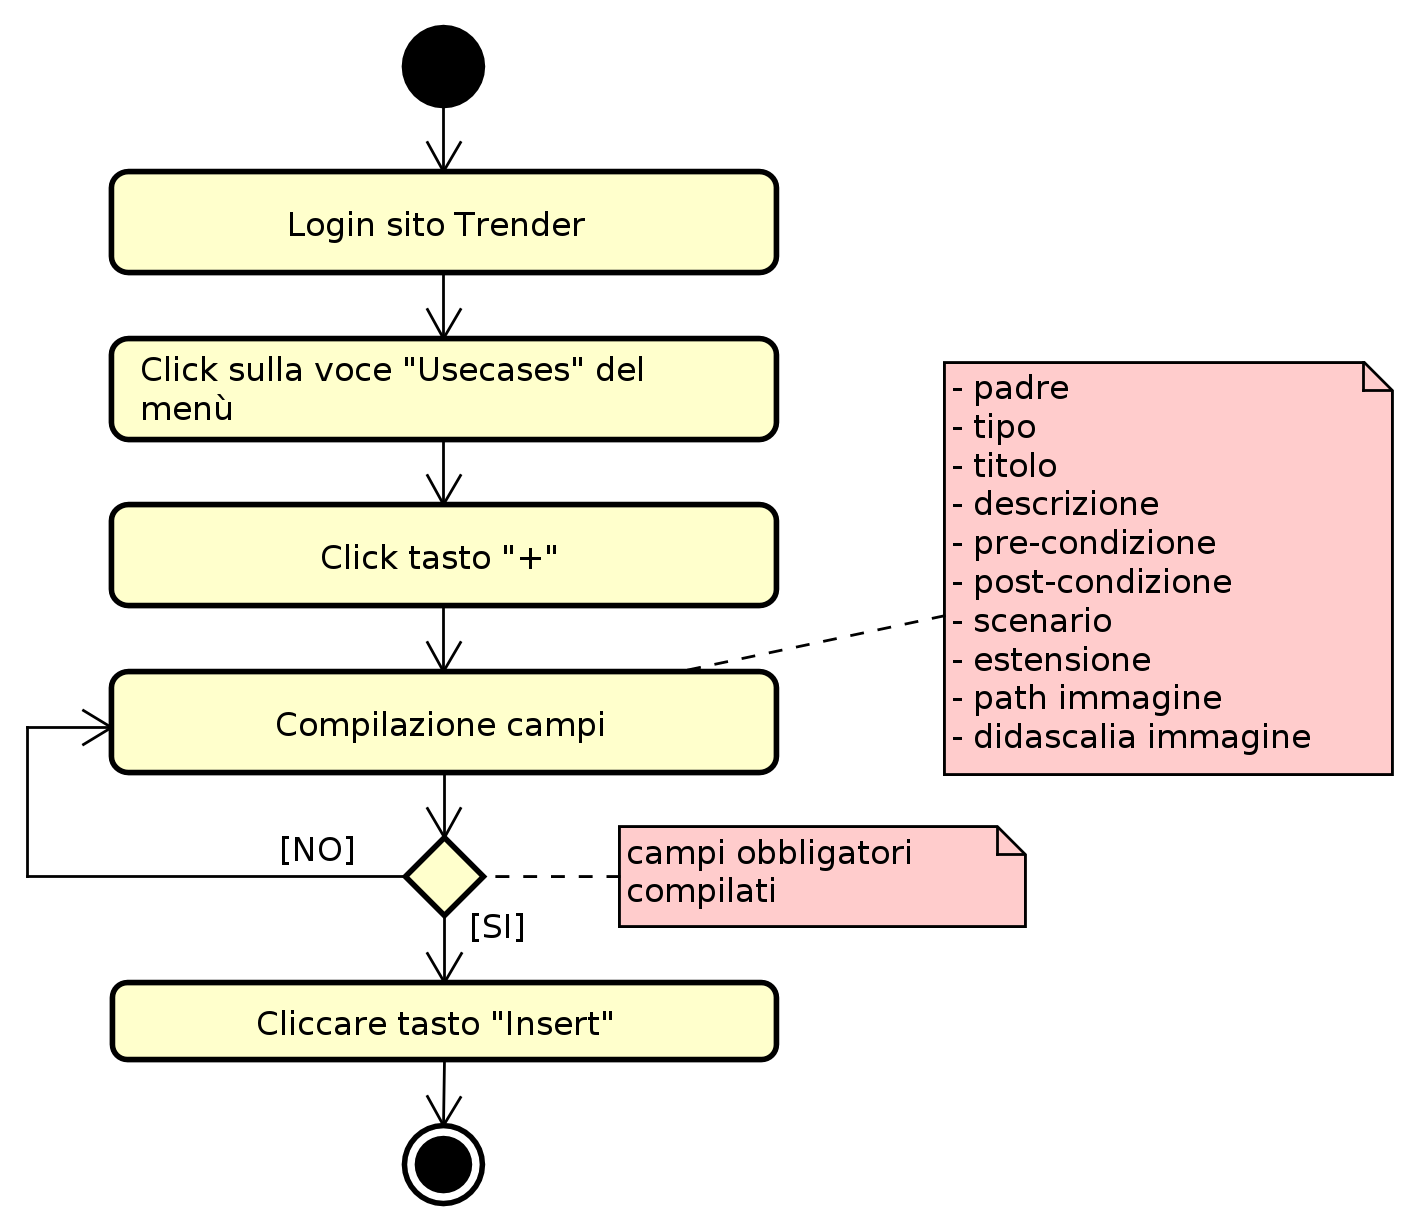
\includegraphics[width=0.7\textwidth]{img/AggiuntaUC}
	    	\caption{Aggiunta use case.}
	    \end{figure}
    
	    \paragraph{Modifica use case su Trender}
	    La modifica di uno use case deve rispettare i seguenti passi:
	    \begin{enumerate}
	    	\item login al sito \url{http://zephyrusar.altervista.org/trender/};
	    	\item cliccare sulla voce del menu: \hicode{Usecases};
	    	\item cliccare sull'\hicode{id} dello use case;
	    	\item modificare i campi: padre, tipo, titolo, descrizione, pre-condizione, post-condizione, scenario, estensione, path immagine, didascalia immagine, associazione use case-attore, associazione use case requisito;
	    	\item cliccare sul tasto \hicode{save}.
	    \end{enumerate}
	    \begin{figure}[H]
	    	\centering
	    	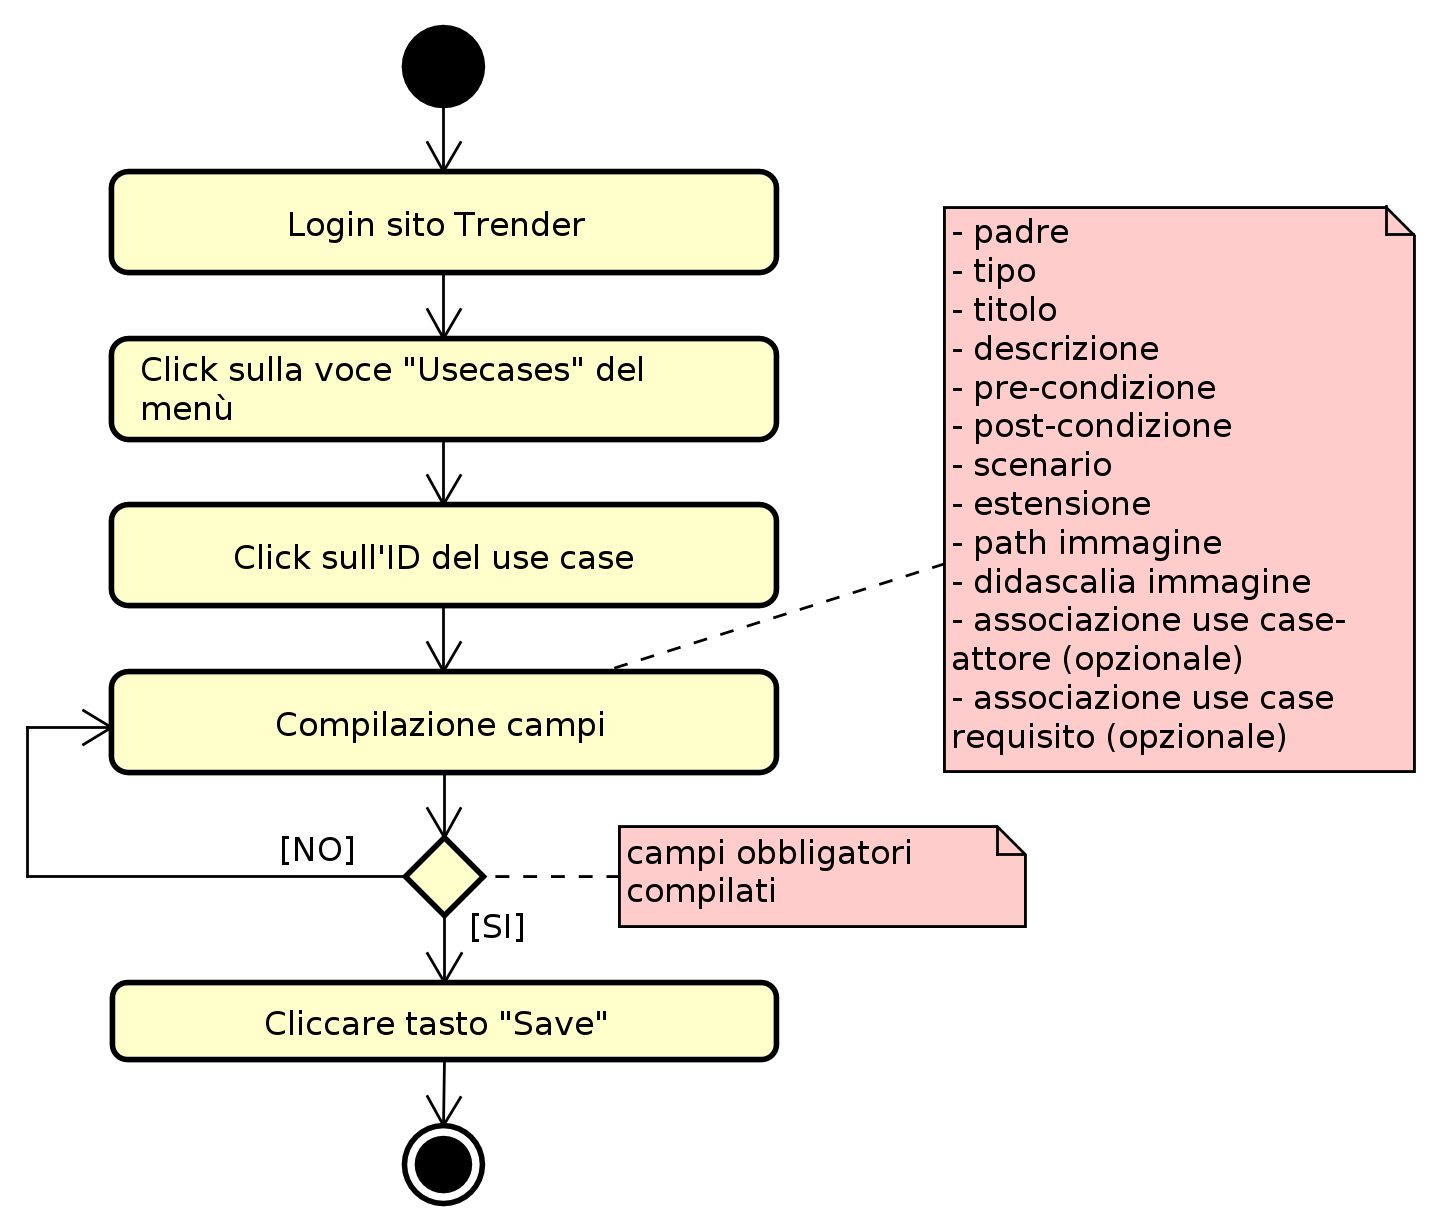
\includegraphics[width=0.7\textwidth]{img/ModificaUC}
	    	\caption{Modifica use case.}
	    \end{figure}
	    
	    \paragraph{Eliminazione use case su Trender}
	    L'eliminazione di uno use case deve rispettare i seguenti passi:
	    \begin{enumerate}
	    	\item login al sito \url{http://zephyrusar.altervista.org/trender/};
	    	\item cliccare sulla voce del menu: \hicode{Usecases};
	    	\item cliccare sull'\hicode{id} dello use case;
	    	\item cliccare sul tasto \hicode{delete use case}.
	    \end{enumerate}

	    \paragraph{Aggiunta requisito su Trender}
	    L'aggiunta di un requisito deve rispettare i seguenti passi:
	    \begin{enumerate}
			\item login al sito \url{http://zephyrusar.altervista.org/trender/};
			\item cliccare sulla voce del menu: \hicode{Requirements};
			\item cliccare sul tasto \hicode{+} rosso, in basso a destra;
			\item compilare i campi: padre, importanza(obbligatorio, desiderabile, facoltativo), tipo(funzionale, prestazionale, qualitativo, vincolo), sorgente, descrizione;
			\item cliccare sul tasto \hicode{insert}.
		\end{enumerate}
		\begin{figure}[H]
			\centering
			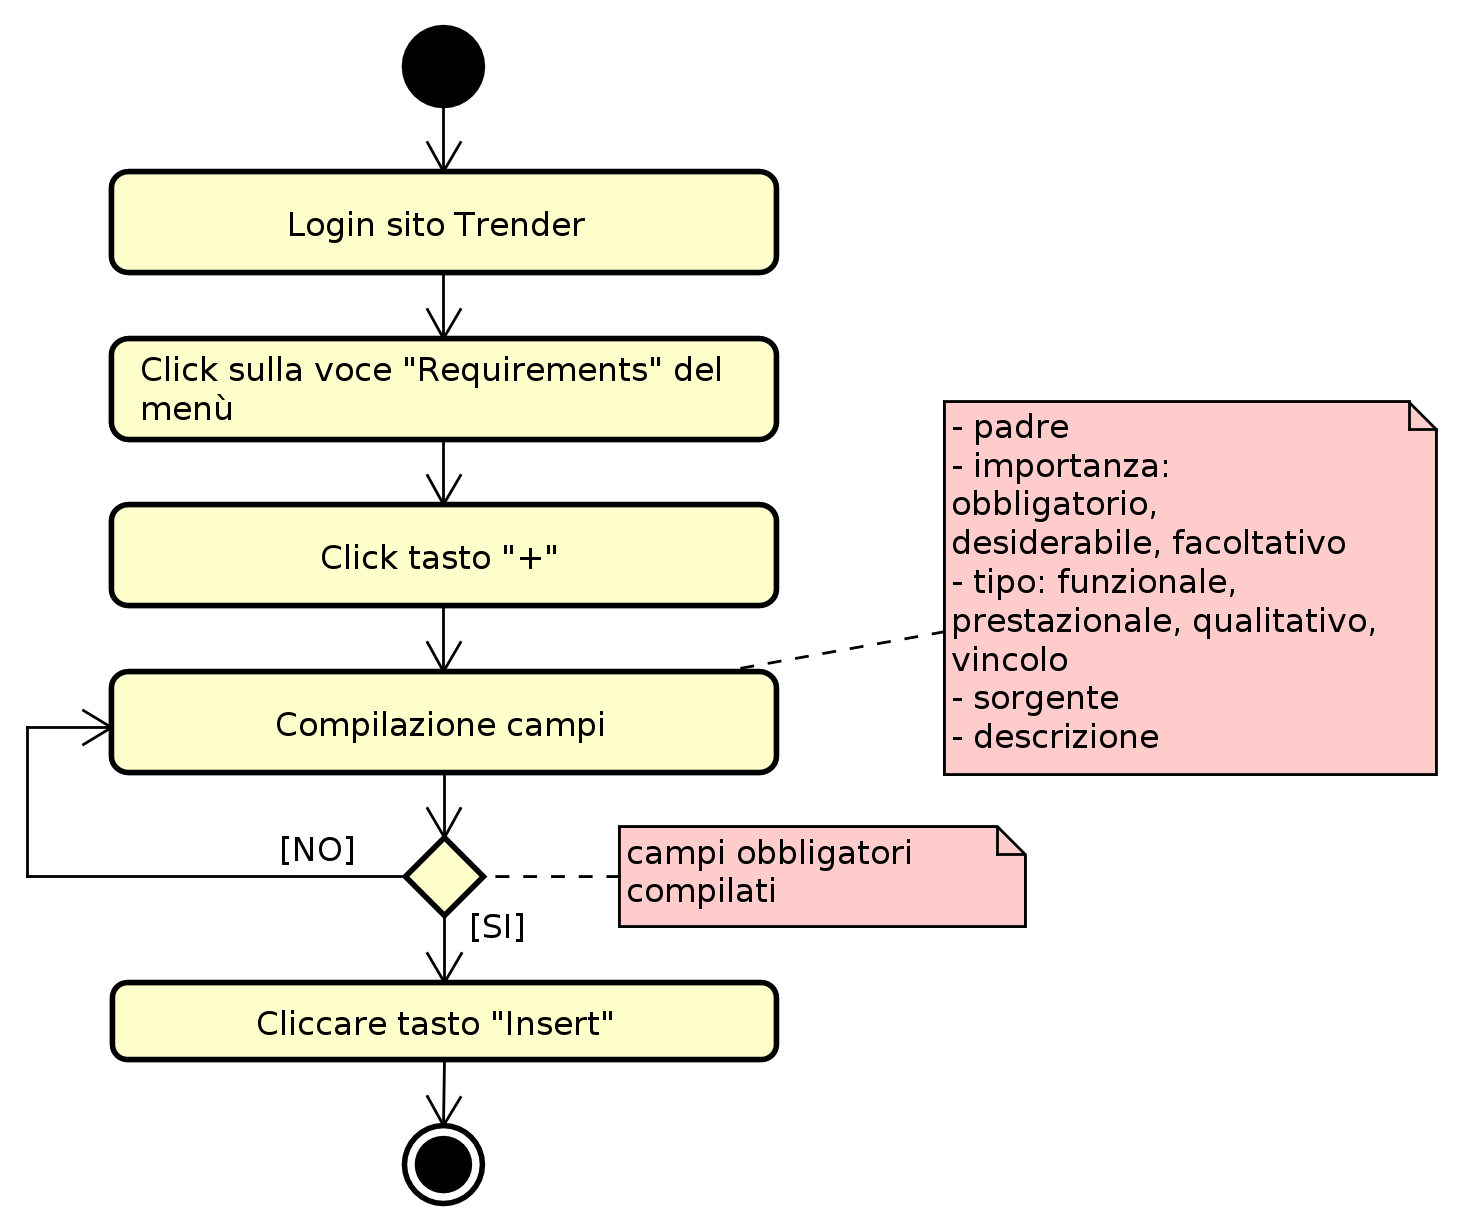
\includegraphics[width=0.7\textwidth]{img/AggiuntaReq}
			\caption{Aggiunta requisito.}
		\end{figure}
			    
		\paragraph{Modifica requisito su Trender}
		La modifica di un requisito deve rispettare i seguenti passi:
		\begin{enumerate}
			\item login al sito \url{http://zephyrusar.altervista.org/trender/};
			\item cliccare sulla voce del menu: \hicode{Requirements};
	    	\item cliccare sull'\hicode{id} del requisito;	
			\item modificare i campi: padre, importanza(obbligatorio, desiderabile, facoltativo), tipo(funzionale, prestazionale, qualitativo, vincolo), sorgente, descrizione, associazione classe (opzionale), package (opzionale), test di sistema (opzionale), test di validazione (opzionale);
			\item cliccare sul tasto \hicode{save}.
		\end{enumerate}
		\begin{figure}[H]
			\centering
			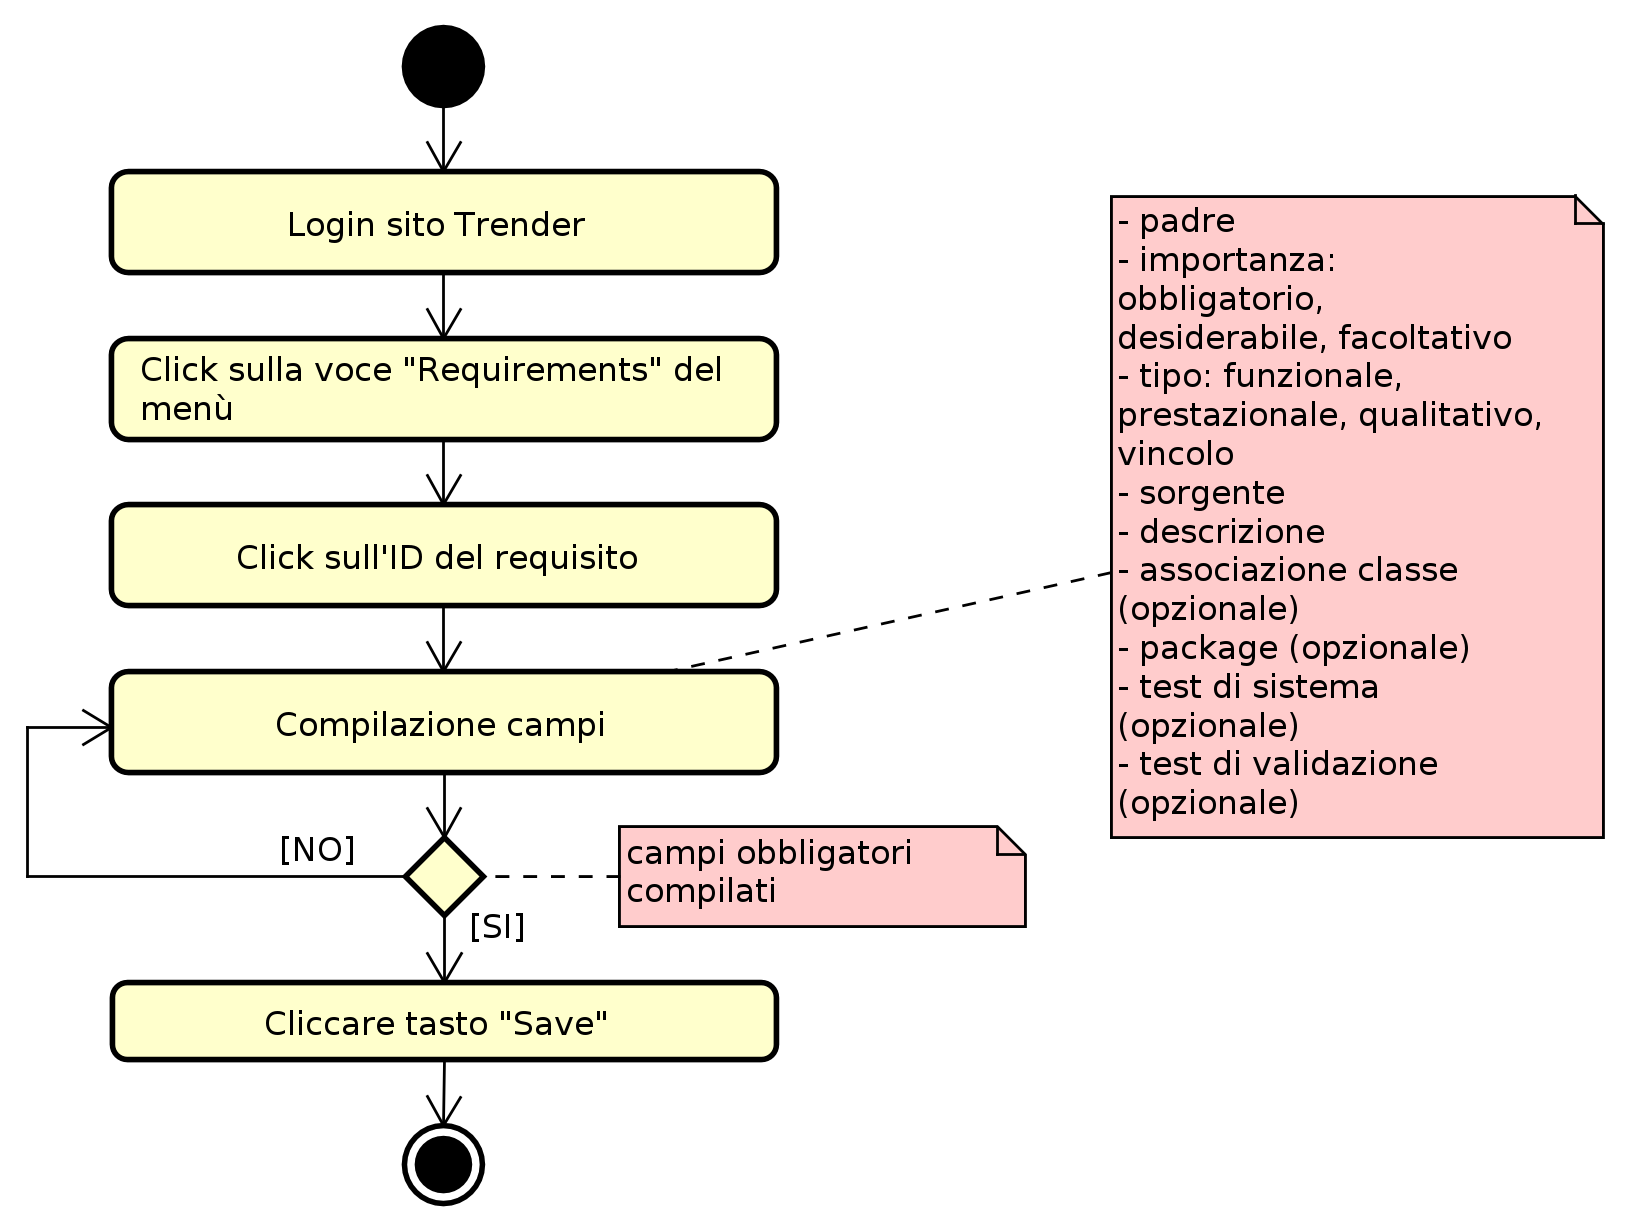
\includegraphics[width=0.7\textwidth]{img/ModificaReq}
			\caption{Modifica requisito.}
		\end{figure}
	
		\paragraph{Eliminazione requisito su Trender}
		L'eliminazione di un requisito deve rispettare i seguenti passi:
		\begin{enumerate}
			\item login al sito \url{http://zephyrusar.altervista.org/trender/};
			\item cliccare sulla voce del menu: \hicode{Requirements};
			\item cliccare sull'\hicode{id} del requisito;
			\item cliccare sul tasto \hicode{delete requirement}.
		\end{enumerate}

		\paragraph{Aggiunta package su Trender} \label{sec:traccComp}
		L'aggiunta di un package deve rispettare i seguenti passi:
		\begin{enumerate}
			\item login al sito \url{http://zephyrusar.altervista.org/trender/};
			\item cliccare sulla voce del menu: \hicode{Packages};
			\item cliccare sul tasto \hicode{+} rosso, in basso a destra;
			\item compilare i campi: nome, descrizione, path immagine, didascalia, padre (opzionale);
			\item cliccare sul tasto \hicode{insert}.
		\end{enumerate}
		\begin{figure}[H]
			\centering
			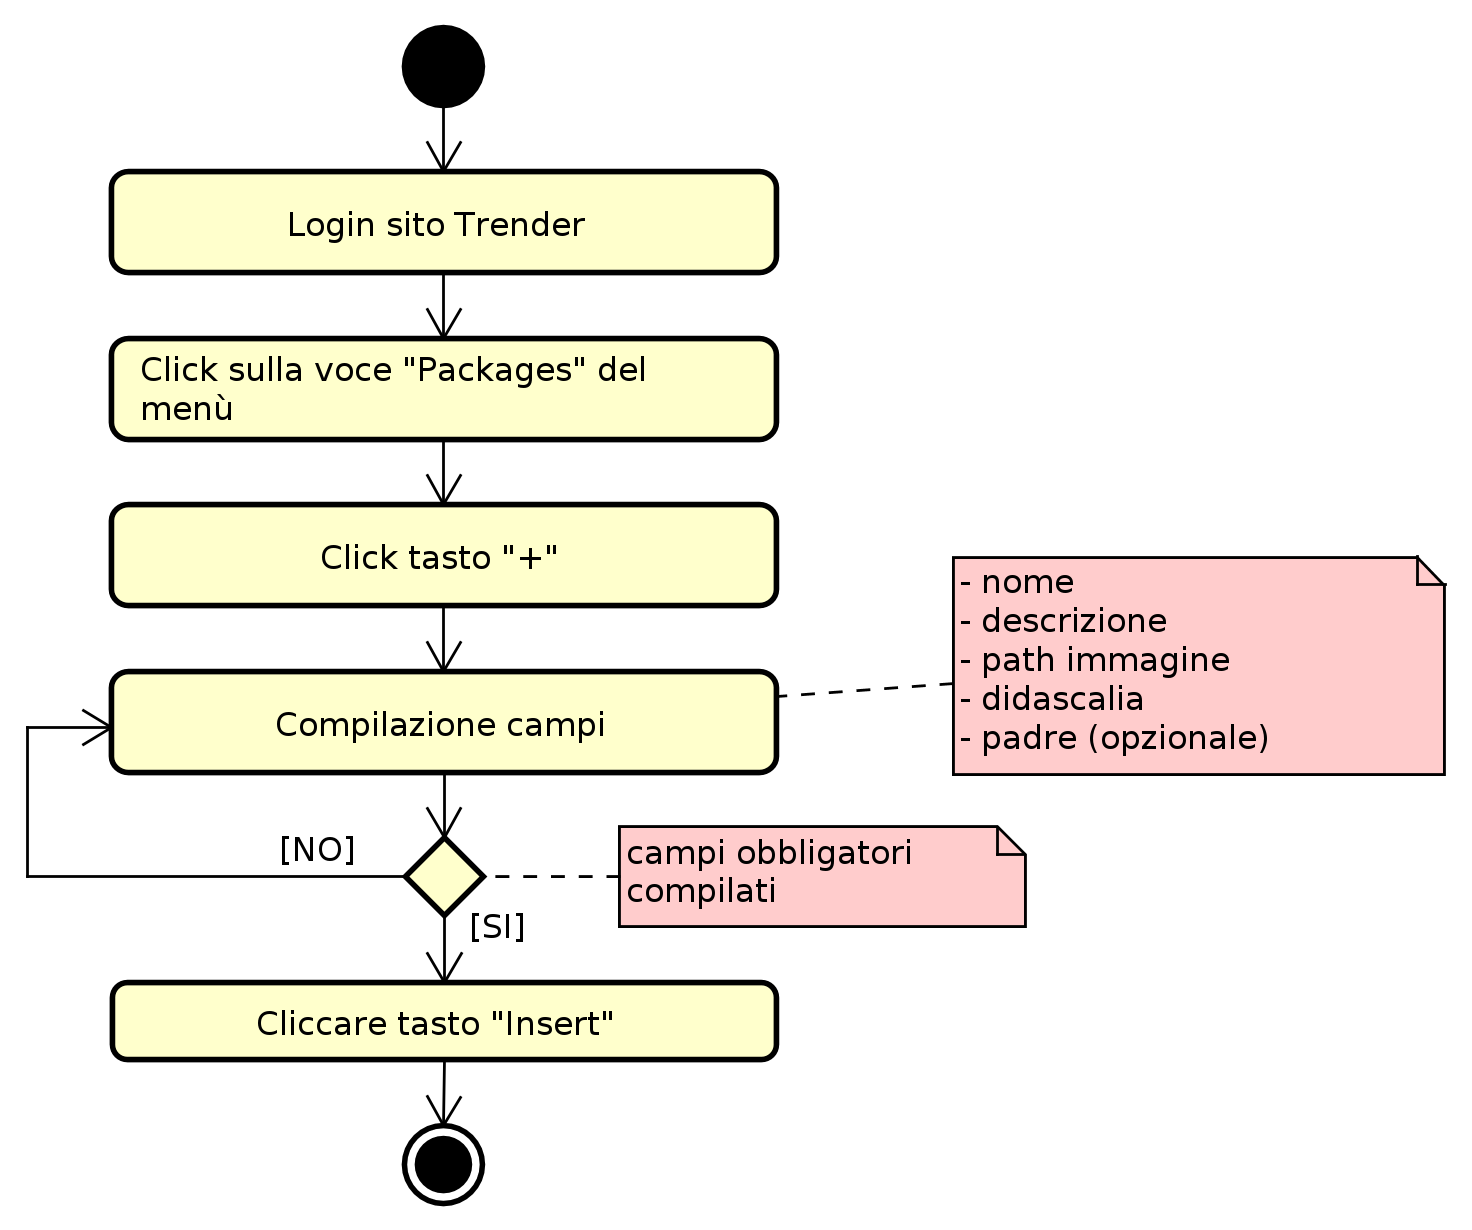
\includegraphics[width=0.7\textwidth]{img/AggiuntaPack}
			\caption{Aggiunta package.}
		\end{figure}
		
		\paragraph{Modifica package su Trender} \label{sec:traccTint}
		La modifica di un package deve rispettare i seguenti passi:
		\begin{enumerate}
			\item login al sito \url{http://zephyrusar.altervista.org/trender/};
			\item cliccare sulla voce del menu: \hicode{Packages};
			\item cliccare sull'\hicode{id} del packages;	
			\item modificare i campi: nome, descrizione, path immagine, didascalia, padre (opzionale), test d'integrazione;
			\item cliccare sul tasto \hicode{save}.
		\end{enumerate}
		\begin{figure}[H]
			\centering
			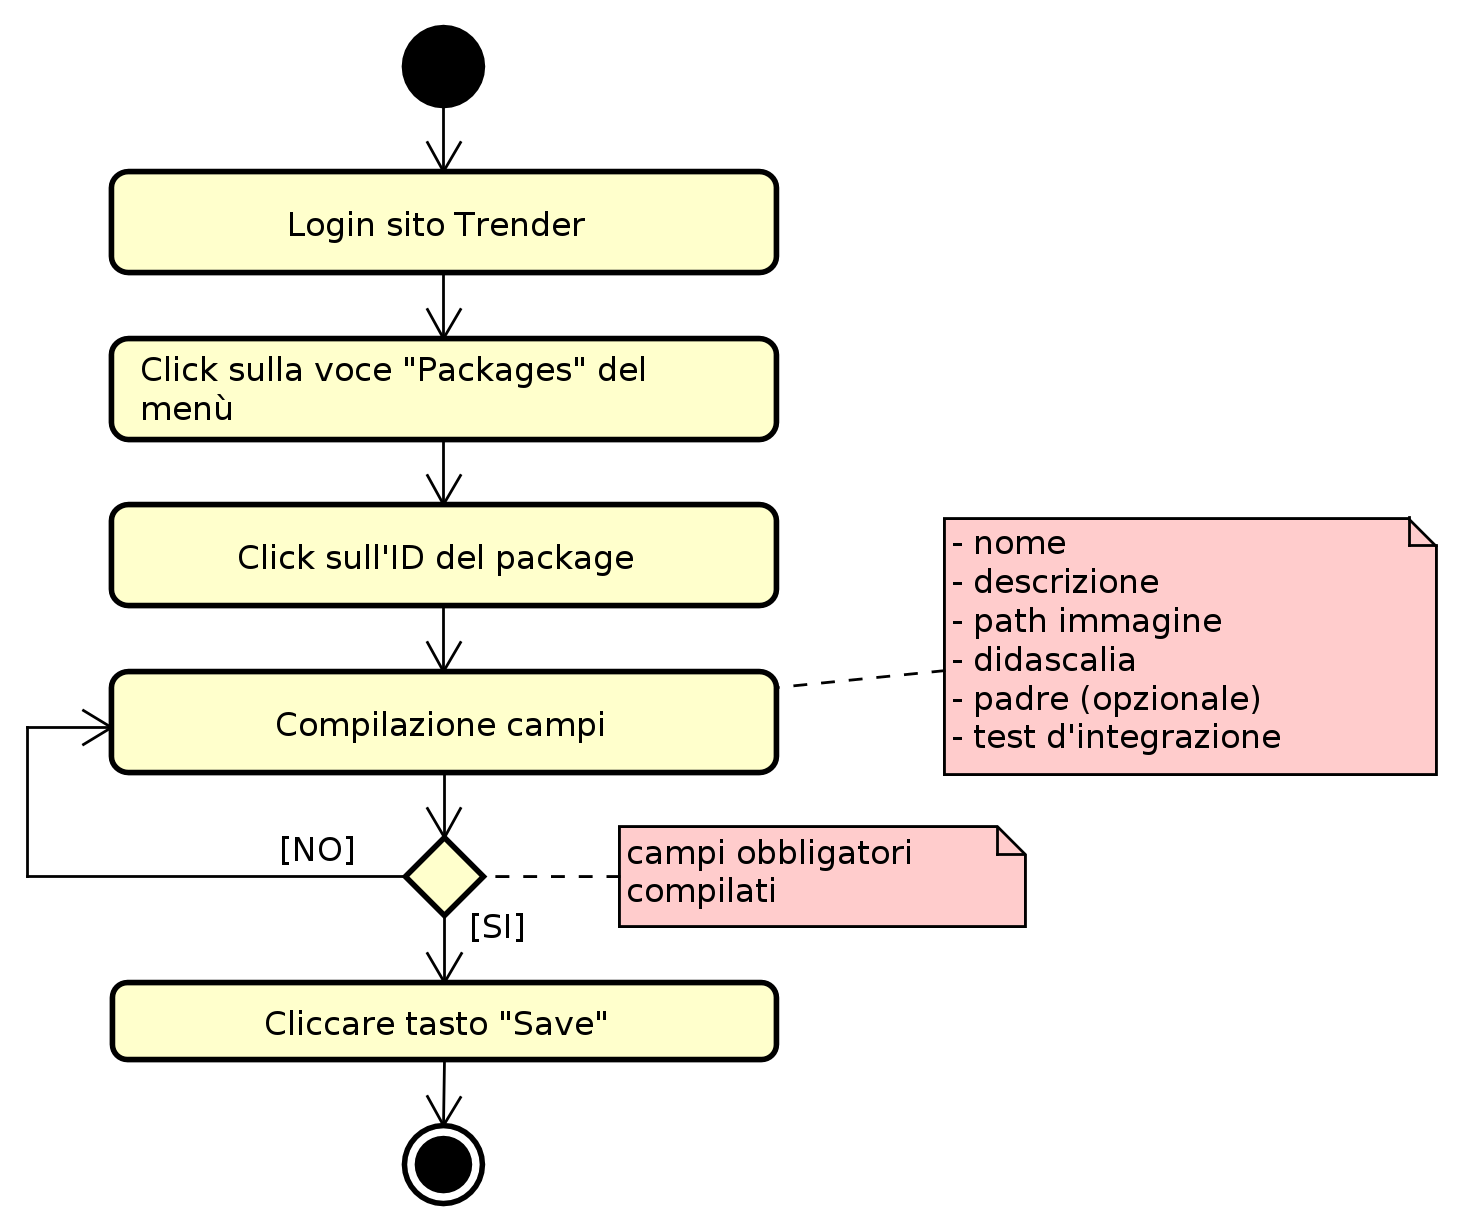
\includegraphics[width=0.7\textwidth]{img/ModificaPack}
			\caption{Modifica package.}
		\end{figure}
	
		\paragraph{Eliminazione package su Trender}				
		L'eliminazione di un package deve rispettare i seguenti passi:
		\begin{enumerate}
			\item login al sito \url{http://zephyrusar.altervista.org/trender/};
			\item cliccare sulla voce del menu: \hicode{Packages};
			\item cliccare sull'\hicode{id} del package;
			\item cliccare sul tasto \hicode{delete package}.
		\end{enumerate}
		
		\paragraph{Aggiunta classe su Trender}
		L'aggiunta di una classe deve rispettare i seguenti passi:
		\begin{enumerate}
			\item login al sito \url{http://zephyrusar.altervista.org/trender/};
			\item cliccare sulla voce del menu: \hicode{Classes};
			\item cliccare sul tasto \hicode{+} rosso, in basso a destra;
			\item compilare i campi: selezione package, nome classe, descrizione, utilizzo;
			\item cliccare sul tasto \hicode{insert}.
		\end{enumerate}
		\begin{figure}[H]
			\centering
			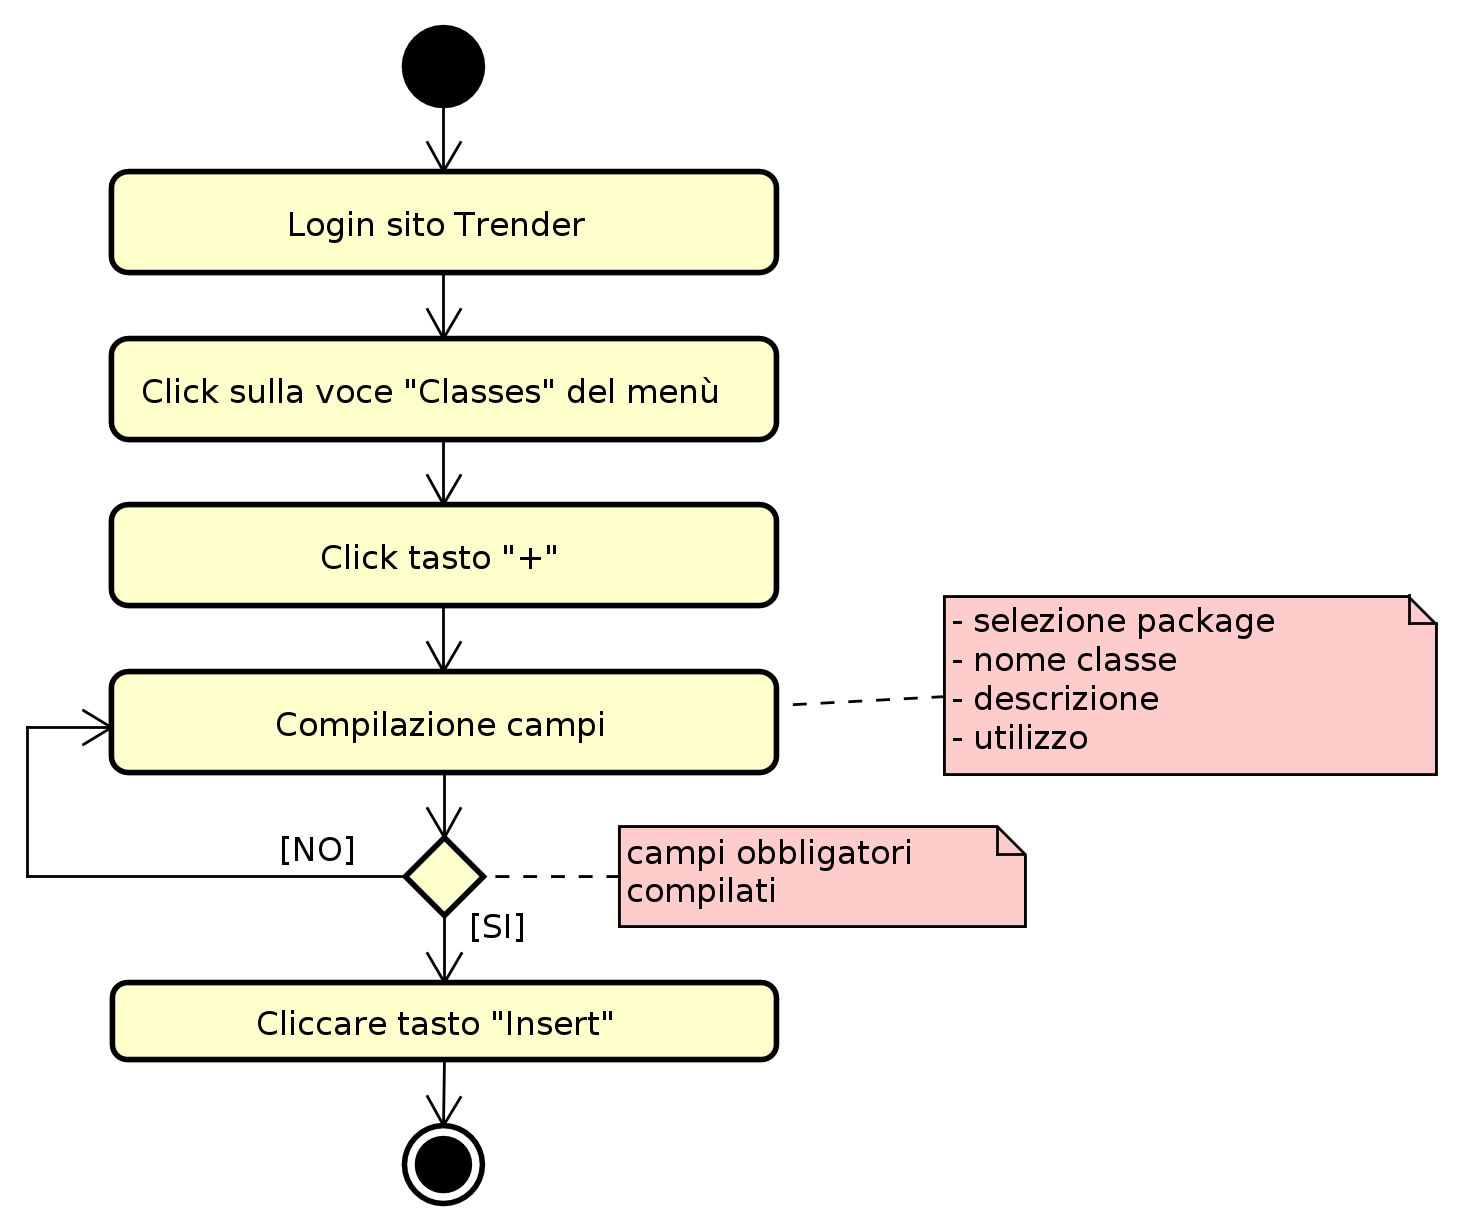
\includegraphics[width=0.7\textwidth]{img/AggiuntaClasse}
			\caption{Aggiunta classe.}
		\end{figure}
		
		\paragraph{Modifica classe su Trender}
		La modifica di una classe deve rispettare i seguenti passi:
		\begin{enumerate}
			\item login al sito \url{http://zephyrusar.altervista.org/trender/};
			\item cliccare sulla voce del menu: \hicode{Classes};
			\item cliccare sull'\hicode{id} della classe;	
			\item modificare i campi: selezione package, nome classe, descrizione, utilizzo, classe base, classe target, tipo relazione, attributi (tipo, nome, descrizione), metodi (tipo di ritorno, segnatura, descrizione, parametri (tipo parametro, nome, descrizione);
			\item cliccare sul tasto \hicode{save}.
		\end{enumerate}
		\begin{figure}[H]
			\centering
			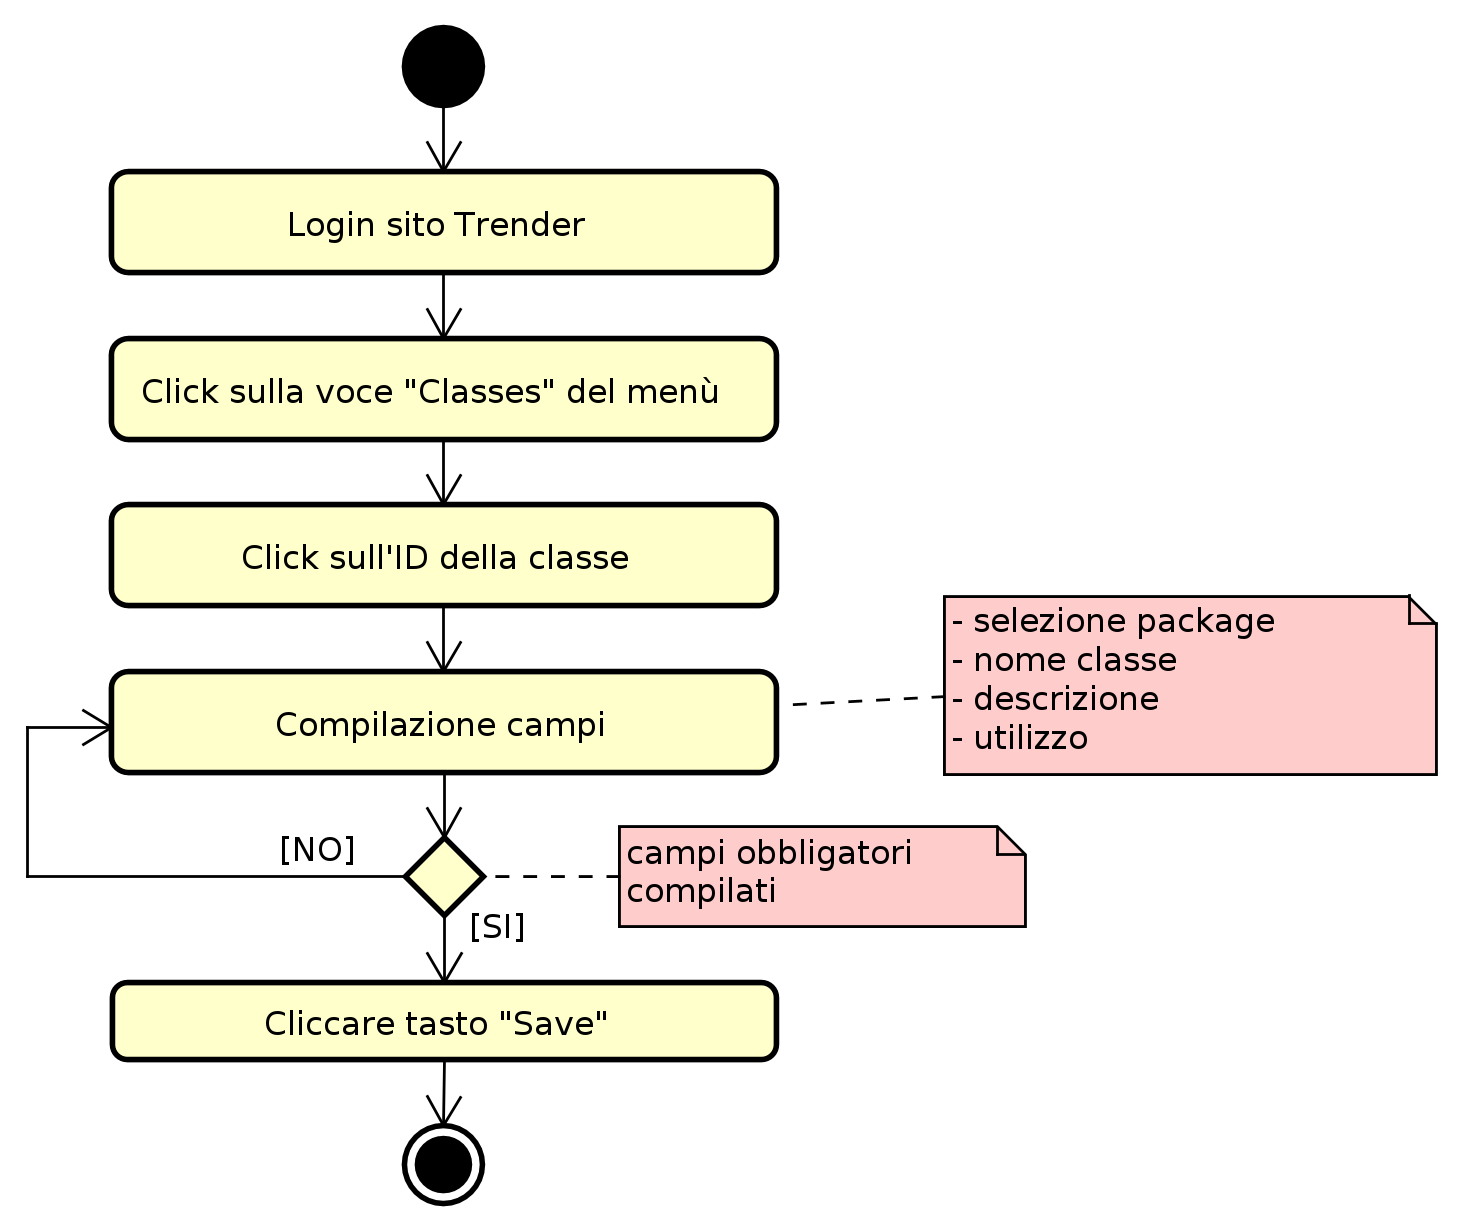
\includegraphics[width=0.7\textwidth]{img/ModificaCl}
			\caption{Modifica classe.}
		\end{figure}
		
		\paragraph{Eliminazione classe su Trender}	
		L'eliminazione di una classe deve rispettare i seguenti passi:
		\begin{enumerate}
			\item login al sito \url{http://zephyrusar.altervista.org/trender/};
			\item cliccare sulla voce del menu: \hicode{Classes};
			\item cliccare sull'\hicode{id} della classe;
			\item cliccare sul tasto \hicode{delete class}.
		\end{enumerate}
		
		\paragraph{Aggiunta test di unità su Trender} \label{sec:traccTuni}
		L'aggiunta di un test di unità deve rispettare i seguenti passi:
		\begin{enumerate}
			\item login al sito \url{http://zephyrusar.altervista.org/trender/};
			\item cliccare sulla voce del menu: \hicode{Test};
			\item cliccare sul tasto \hicode{+} rosso, in basso a destra;
			\item compilare i campi: package, classe, metodo da combinare, descrizione del test;
			\item cliccare sul tasto \hicode{insert}.
		\end{enumerate}
		\begin{figure}[H]
			\centering
			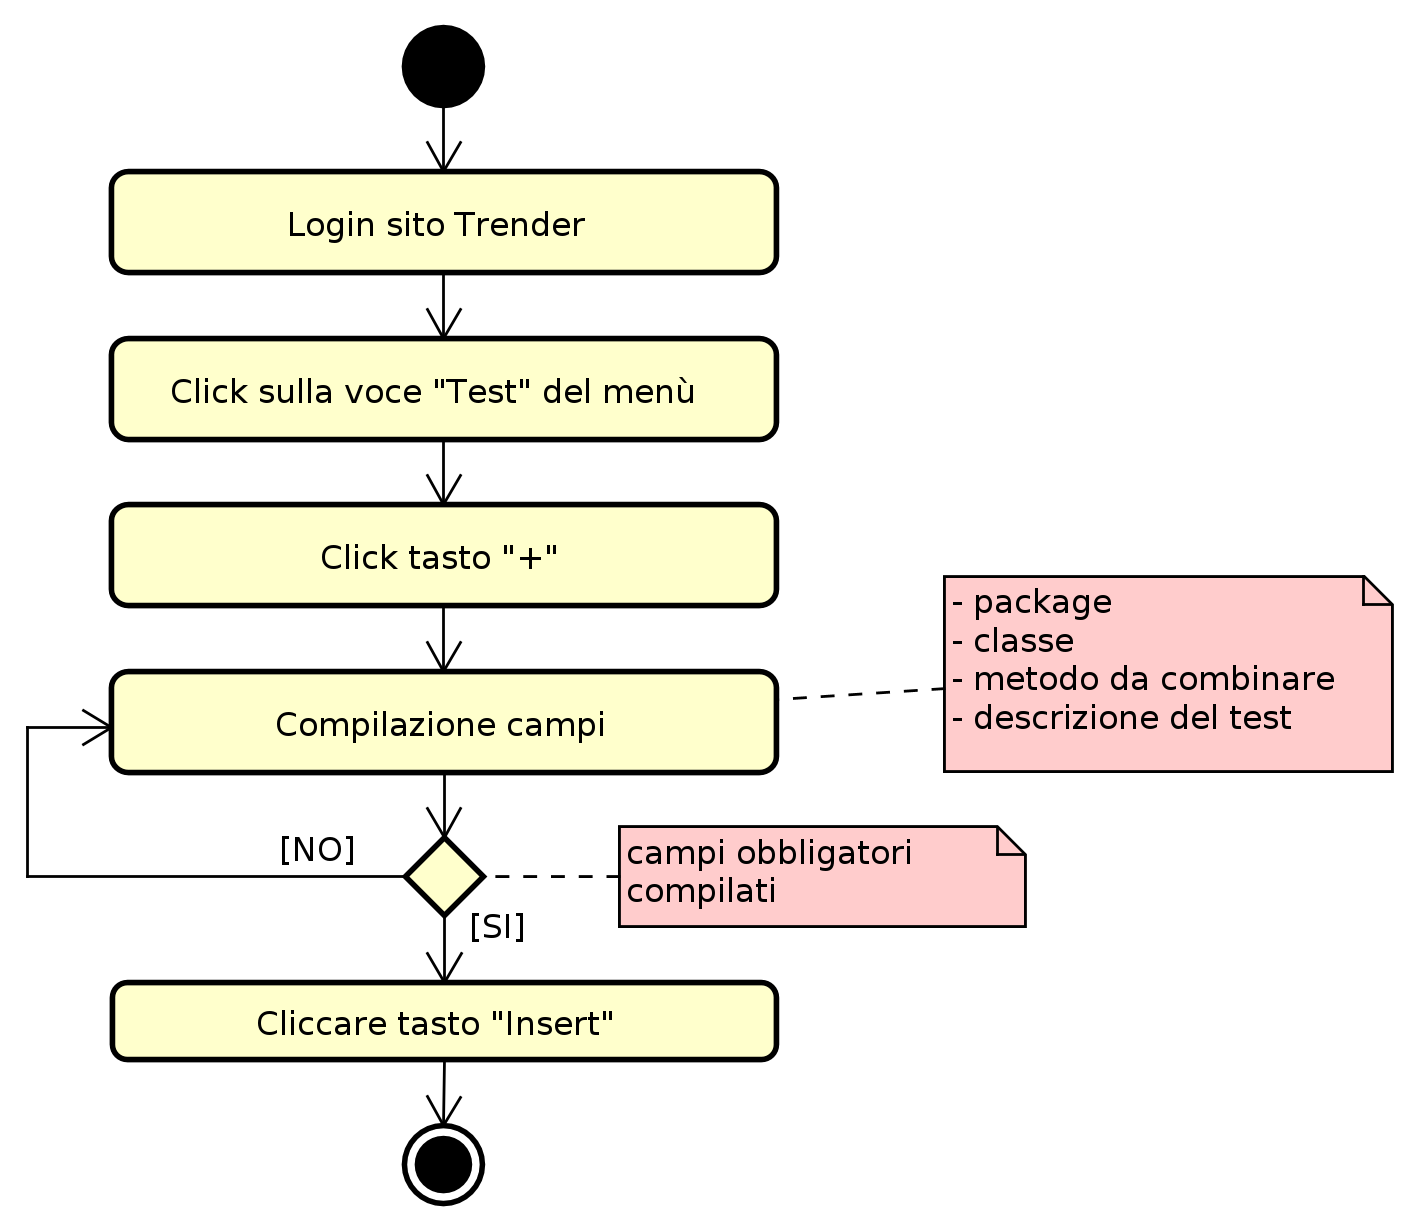
\includegraphics[width=0.7\textwidth]{img/AggiuntaTestUnit}
			\caption{Aggiunta test di unità.}
		\end{figure}

		\paragraph{Modifica ed eliminazione Test di unità su Trender}
		Questa funzionalità non è stata implementata, pertanto bisogna effettuare la modifica dei campi dati del test o l'eliminazione attraverso l'interfaccia di PhpMyAdmin selezionando la tabella: \texttt{UnitTest}.
		%
		\paragraph{Esportazione da Trender a codice \LaTeX}
		L'esportazione del codice \LaTeX{} da Trender deve rispettare i seguenti passi:
		\begin{enumerate}
			\item login al sito \url{http://zephyrusar.altervista.org/trender/};
			\item cliccare sulla voce del menu: \hicode{Prints};
			\item selezionare i campi desiderati per la stampa (di solito tutti);
			\item cliccare sul tasto \hicode{print all};
			\item selezionare la sezione del codice \LaTeX{} da visualizzare;
			\item copiare il codice \LaTeX e incollarlo sul documento desiderato.
		\end{enumerate}
		\begin{figure}[H]
			\centering
			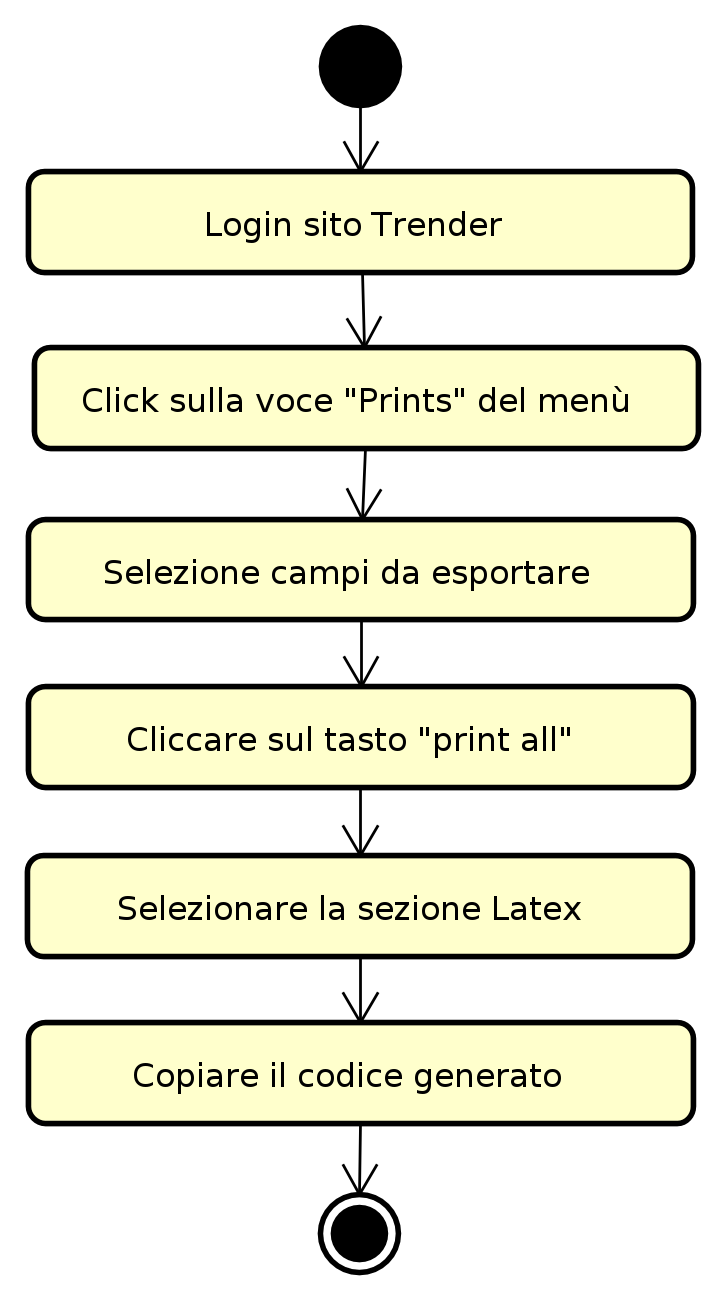
\includegraphics[width=0.3\textwidth]{img/Export}
			\caption{Esportazione codice \LaTeX{} da Trender.}
		\end{figure}
		%
		\paragraph{Impostazioni Trender}
		Alcune impostazioni di Trender si possono modificare rispettando i seguenti passi:
		\begin{enumerate}
			\item login al sito \url{http://zephyrusar.altervista.org/trender/};
			\item cliccare sulla voce del menu a forma di ingranaggio;
			\item inserire la sorgente dei requisiti: nome sorgente.
		\end{enumerate}
		%
		\paragraph{Configurazione WebStorm}
		Lo stile di codifica adottato (vedi sezione \ref{codeStyle}) e personalizzato per questo progetto deve essere importato all'interno di WebStorm nel tool ESLint. Per fare questo è necessario seguire i seguenti passaggi:
		\begin{enumerate}
			\item aprire WebStorm;
			\item aprire il menu \hicode{File -> Preferences};
			\item entrare nel menu \hicode{Language \& Frameworks->JavaScript->Code Quality Tools->ESLint};
			\item abilitare il tool essicurandosi di aver installato prima Node.js (vedi sezione \ref{nodejs});
			\item selezionare nel campo ESLint package il file che si trova all'interno del progetto \hicode{DeGeOp/node\_modules/eslint};
			\item salvare le impostazioni premendo il tasto \hicode{Ok}.
		\end{enumerate}
		


\section{Processi di supporto}
    \subsection{Documentazione}
        \subsubsection{Scopo}
        Lo scopo del processo di documentazione è di redigere e mantenere la documentazione durante l'intero \glo{Ciclo di vita}{ciclo di vita} del software. La corretta implementazione del processo deve:
        \begin{itemize}
            \item dare una chiara visione dei documenti che devono essere prodotti durante il ciclo di vita del software;
            \item fornire le norme necessarie alla stesura dei documenti;
            \item produrre documenti formali coerenti.
        \end{itemize}
        \subsubsection{Template}
        È stato creato un template \glo{Latex}{\LaTeX{}} per garantire che tutti i documenti creati dal \glo{Gruppo}{gruppo} abbiano la stessa struttura grafica e lo stesso stile di formattazione. Ogni membro del gruppo deve creare i documenti richiesti utilizzando tale template e deve ridurre al minimo indispensabile eventuali variazioni personali nella formattazione.
        \subsubsection{Struttura dei documenti} \label{sec:strutturaDoc}
                \paragraph{Prima pagina}
                La prima pagina di ogni documento deve presentare la seguente struttura:
                \begin{itemize}
                    \item logo del gruppo;
                    \item titolo del documento;
                    \item informazioni del documento:
                    \begin{itemize}
                        \item versione;
                        \item data di creazione;
                        \item data di ultima modifica;
                        \item stato del documento;
                        \item redattori del documento;
                        \item verificatori;
                        \item responsabile approvazione;
                        \item lista di distribuzione;
                        \item email del gruppo.
                    \end{itemize}
                \end{itemize}
                \paragraph{Registro delle modifiche}
                La seconda pagina di ogni documento formale deve contenere una tabella con la lista delle modifiche apportate al documento. Ogni riga della tabella deve essere compilata per intero con le seguenti informazioni:
                \begin{itemize}
                    \item versione del documento successiva alla modifica;
                    \item data in cui è stata eseguita la modifica;
                    \item autore della modifica;
                    \item ruolo dell'autore;
                    \item descrizione concisa della modifica apportata.
                \end{itemize}
                \paragraph{Indice}
                Nella pagina successiva alla fine del registro delle modifiche ogni documento formale deve contenere l'indice dei suoi contenuti; tale indice deve permettere la lettura \glo{Ipertestuale}{ipertestuale} del documento. L'indice deve essere numerato a partire da 1, ogni sottosezione riparte da 1 e aggiunge il proprio indice a quello del padre separandolo con un punto. Eventuali appendici invece di essere numerate saranno indicate con lettere maiuscole a partire da A seguendo l'ordine alfabetico internazionale.
                \paragraph{Note a piè di pagina}
                Eventuali note vanno indicate in basso a sinistra nella pagina in cui compaiono con il loro numero identificativo e la loro descrizione.
                \paragraph{Contenuto principale}
                Tutte le pagine successive all'indice del documento devono contenere un'intestazione e un piè di pagina.
                L'intestazione deve contenere:
                \begin{itemize}
                    \item nome della sezione allineato a sinistra;
                    \item nome del documento allineato a destra.
                \end{itemize}
                Il piè di pagina deve contenere:
                \begin{itemize}
                    \item nome del gruppo e del progetto allineati a sinistra;
                    \item pagina corrente rispetto alle pagine totali del documento allineate a destra.
                \end{itemize}
        \subsubsection{Norme tipografiche} \label{sec:normeTipografiche}
                \paragraph{Glossario}
                Ogni parola contenuta nel \gl{} deve essere scritta in corsivo e contrassegnata da una "G" a pedice come da esempio:\\
                \centerline{\textit{termine\textsubscript{G}}}
                
                \paragraph{Stile del testo}
                Per facilitare la stesura del documento, migliorarne correttezza e leggibilità, TexStudio mette a disposizione dei tool per il controllo grammaticale. Ogni membro del gruppo deve controllare nelle impostazioni del proprio strumento che siano attivati:
                \begin{itemize}
                	\item \textbf{individua ripetizioni:} durante la scrittura del documento, se una parola viene ripetuta troppo viene sottolineata di verde;
                	\item \textbf{individua errori ortografici:} gli errori vengono sottolineati di rosso;
                	\item \textbf{lingua predefinita:} italiano.
                \end{itemize}
                Le seguenti convenzioni devono essere rispettate nella stesura dei documenti:
                \begin{itemize}
                    \item \textbf{grassetto:} deve essere utilizzato nei seguenti casi:
                        \begin{itemize}
                            \item titoli di sezioni e paragrafi;
                            \item termini di elenchi puntati per i quali si fornisce una descrizione;
                            \item riferimenti alle revisioni di avanzamento.
                        \end{itemize}
                    \item \textbf{corsivo:} deve essere utilizzato nei seguenti casi:
                        \begin{itemize}
                            \item nome del gruppo;
                            \item nome del proponente;
                            \item nome del progetto;
                            \item citazioni;
                            \item abbreviazioni;
                            \item parole presenti nel glossario;
                            \item ruoli del progetto;
                            \item nomi dei documenti.
                        \end{itemize}
                    \item \textbf{monospace:} deve essere utilizzato nei seguenti casi:
                        \begin{itemize}
                            \item nomi di file;
                            \item codice di programmazione;
                            \item indirizzi email.
                        \end{itemize}
                    \item \textbf{maiuscolo:} le uniche parole che possono essere scritte interamente a caratteri maiuscoli sono gli acronimi e le sigle.
                \end{itemize}
                \paragraph{Titoli}
                I titoli delle sezioni e dei paragrafi vanno scritti con solo la prima lettera maiuscola a meno di nomi propri e di termini indicati nella sezione \ref{sec:formati}.
                \paragraph{Elenchi puntati}
                Le seguenti convenzioni devono essere rispettate nella creazione di elenchi puntati:
                \begin{itemize}
                    \item ogni elemento dell'elenco deve iniziare con la lettera minuscola a meno che non sia un nome proprio;
                    \item ogni elemento dell'elenco tranne l'ultimo deve terminare con un punto e virgola;
                    \item l'ultimo elemento dell'elenco deve terminare con il punto.
                \end{itemize}
                \paragraph{Formati}\label{sec:formati}
                I seguenti formalismi devono essere utilizzati durante la stesura dei documenti:
                \begin{itemize}
                    \item \textbf{date:} le date presenti nei documenti devono seguire lo standard \glo{ISO}{ISO} 8601:2004 (vedi riferimento \ref{sec:iso8601}):\\\\
                    \centerline{YYYY-MM-GG}\\
                    dove:
                    \begin{itemize}
                        \item \textbf{YYYY:} rappresenta l'anno espresso con quattro cifre;
                        \item \textbf{MM:} rappresenta il mese espresso con due cifre;
                        \item \textbf{GG:} rappresenta il giorno espresso con due cifre.
                    \end{itemize}
                    È possibile utilizzare il comando \LaTeX{} \texttt{\textbackslash frmdata\{GG\}\{MM\}\{YYYY\}} per la formattazione delle date.
                    \item \textbf{orari:} gli orari presenti nei documenti devono seguire lo standard ISO 8601:2004 (vedi riferimento \ref{sec:iso8601}):\\\\
                    \centerline{hh:mm}\\
                    dove:
                    \begin{itemize}
                        \item \textbf{hh:} rappresentano le ore espresse con due cifre da 00 a 23;
                        \item \textbf{mm:} rappresentano i minuti espressi con due cifre da 00 a 59.
                    \end{itemize}
                    È possibile utilizzare il comando \LaTeX{} \texttt{\textbackslash frmora\{hh\}\{mm\}} per la formattazione delle ore.
                    \item \textbf{valute:} le valute presenti nei documenti devono essere scritte utilizzando il simbolo della valuta usata seguito dal numero. Le cifre decimali devono essere separate dalla virgola, le cifre non decimali devono essere separate da un punto a gruppi di tre:
                    \centerline{[Simbolo valuta] 1.234.567,89}
                    Ad esempio: € 3.869,25
                    \item \textbf{nomi ricorrenti:}
                    I seguenti termini ricorrenti vanno sempre inseriti con i relativi comandi \LaTeX{} forniti dal template (vedi appendice \ref{ComandiLatex}) per garantire omogeneità in tutti i documenti: 
                    \begin{itemize}
                        \item nome del gruppo;
                        \item email di riferimento del gruppo;
                        \item nome del proponente;
                        \item nome del progetto svolto;
                        \item ruoli di progetto;
                        \item nomi dei documenti senza versione;
                        \item nomi dei documenti con versione;
                        \item revisioni di avanzamento del progetto;
                        \item nomi di strumenti o tecnologie.
                    \end{itemize}
                \end{itemize}
                \paragraph{Nomi propri}
                    I nomi propri di persona devono essere scritti come nome e cognome.
        \subsubsection{Componenti grafiche} \label{sec:normeGrafiche}
                \paragraph{Tabelle}
                Tutte le tabelle devono avere un indice numerico univoco che le identifichi all'interno del documento ed una breve didascalia. Le tabelle devono essere centrate orizzontalmente.
                \begin{itemize}
				\item Le tabelle semplici vengono riportate con il comando:
				\begin{verbatim}
				\begin{tabular}[H]
					...
				\end{tabular}
				\end{verbatim}
				dove:
				\begin{itemize}
					\item \textbf{[H]:} è una preferenza di collocazione per oggetti mobili e sta a indicare di inserire la tabella esattamente nel punto dove si vuole che compaia. Per altri parametri quali: t,b,p,! si veda la guida \LaTeX nella sezione \ref{sec:guidalatex}. 
				\end{itemize} 
				\item Le tabelle su più pagine vengono riportate con il comando:
				\begin{verbatim}
					\begin{longtable}
					\endfirsthead
					\endhead
					...
					\end{longtable}
				\end{verbatim}
				dove:
				\begin{itemize}
					\item \textbf{\textbackslash endfirsthead:} specifica l'intestazione della tabella nella prima pagina in cui compare;
					\item \textbf{\textbackslash endhead:} specifica l'intestazione della tabella dalla seconda pagina in poi.
				\end{itemize} 
				\item Le tabelle multiriga e multicolonna vengono riportate con il comando: \\ \\
				\begin{minipage}{9cm}
				\begin{verbatim}
					\begin{tabular}[H]{lccc}
					\toprule
					\multirow {2}*{Elemento} & 
					\multicolumn{3}{c}{Strati} \\
					\cmidrule(lr){2-4}	
					             & K & L & M \\
					\midrule 
					idrogeno     & $1$ &  &  \\
					litio        & $2$ & $1$ &  \\
					sodio        & $2$ & $8$ & $1$  \\ 
					\bottomrule
					\end{tabular}
				\end{verbatim}
				\end{minipage}
				\begin{minipage}[c]{4.3cm}
					che produce la seguente tabella d'esempio: \\ \\
					\begin{tabular}[c]{lccc}
						\toprule
						\multirow {2}*{Elemento} & \multicolumn{3}{c}{Strati} \\
						\cmidrule(lr){2-4}	
						&  K  &  L  &       M        \\
						\midrule 
						idrogeno                  & $1$ &     &  \\
						litio                          & $2$ & $1$ &  \\
\						sodio                       & $2$ & $8$ &      $1$       \\ 
						\bottomrule
					\end{tabular}
				\end{minipage}
			\end{itemize}
		
                \paragraph{Immagini}
                Tutte le immagini inserite all'interno di un documento devono avere ampi margini orizzontali che le separino in modo netto dai paragrafi precedenti e successivi per migliorare la leggibilità. Le immagini devono essere centrate orizzontalmente e devono avere larghezza fissa. I diagrammi \glo{UML}{UML} devono essere inseriti nei documenti come immagini.
                \begin{itemize}
                	\item Le immagini vengono inserite con il seguente comando:
                	\begin{verbatim}
					\begin{figure}[H]
						\includegraphics[width=0.8\textwidth]{img/nomeImmagine}
						\caption{Descrizione \ref{sec:ciclodivitadoc}}
						\label{fig:ciclovitadoc}
					\end{figure}\mbox{}\\
                	\end{verbatim}
                		\begin{itemize}
                		\item \textbf{[H]:} come descritto sopra per le tabelle;
                		\item \textbf{\textbackslash caption:} specifica la didascalia dell'immagine;
                		\item \textbf{[width=0.8\textbackslash textwidth]:} specifica la dimensione dell'immagine, che in questo esempio ricopre l'80\% della larghezza del corpo del documento. Si può esprimere con dei valori che vanno da 0 a 1. 
                	\end{itemize} 
                 \end{itemize}
        \subsubsection{Classificazione dei documenti}\label{sec:classDoc}
            \paragraph{Documenti informali}
            Tutti i documenti non ancora approvati dal responsabile di progetto sono da ritenersi informali e pertanto ad uso unicamente interno.
            \paragraph{Documenti formali}
            Un documento diventa formale in seguito all'approvazione da parte del \responsabilediprogetto. Solo i documenti formali possono essere distribuiti all'esterno del gruppo. Prima di poter essere approvato un documento deve essere verificato come descritto nella sezione \ref{sec:ciclodivitadoc} e secondo le procedure descritte nella sezione \ref{sec:verifica}.
            \paragraph{Glossario} \label{sec:normeGlossario}
            Il \gl{} ha lo scopo di chiarire il significato di alcuni termini calati in un determinato contesto. Al suo interno ci sono parole presenti nei documenti e per rientrarci devono avere le seguenti caratteristiche:
            \begin{itemize}
            	\item trattare argomenti tecnici;
            	\item essere sigle;
            	\item descrivere argomenti sconosciuti o ambigui;
            	\item essere strumenti utilizzati nel progetto.
            \end{itemize} 
	        Ogni termine deve essere accompagnato dalla sua spiegazione chiara, concisa e meno ambigua possibile, lunga al massimo dieci righe. Siccome l'inserimento di un termine a glossario può avvenire durante la stesura di un documento, per evitare confusione, si può anche inserire solamente il termine senza la spiegazione (come descritto nella sezione \ref{sec:insTermine}). Si deve comunque completare la spiegazione il prima possibile.
            \paragraph{Verbali}\label{sec:verbali}
            Per ogni incontro deve essere nominato un segretario che si occuperà della stesura di un verbale. Il verbale deve contenere i seguenti punti:
            \begin{itemize}
                \item \textbf{estremi della riunione:}
                    \begin{itemize}
                        \item data;
                        \item ora inizio;
                        \item ora fine;
                        \item luogo dove si è svolto l'incontro;
                        \item lista dei partecipanti;
                        \item lista degli assenti con eventuali motivazioni;
                        \item nome del segretario.
                    \end{itemize}
                \item \textbf{ordine del giorno:} elenco degli argomenti che saranno discussi;
                \item \textbf{corpo del verbale:} verbale dell'incontro;
                \item \textbf{decisioni prese:} elenco delle decisioni prese identificate in modo univoco.
            \end{itemize}
            Una volta approvato dal \responsabilediprogetto{} il verbale deve essere distribuito a tutti i componenti del gruppo; I varbali esterni dovranno essere inviati anche al proponente.
            I nomi dei file dei verbali devono rispettare il seguente formato:\\\\
            \centerline{\texttt{Verbale[Tipologia]\_[ID]\_[Data riunione].pdf}}\\
            dove:
            \begin{itemize}
                \item \textbf{tipologia:} \texttt{Esterno} o \texttt{Interno};
                \item \textbf{ID:} identificativo numerico, si distingue tra verbali interni ed esterni, parte da 1;
                \item \textbf{data riunione:} data in cui si è svolta la riunione in formato YYYYMMGG.
            \end{itemize}
	        I nomi delle decisioni devono rispettare il seguente formato:\\\\
            \centerline{\texttt{V[ID tipologia]\_[ID].[Numero decisione]}}\\
            dove:
            \begin{itemize}
            	\item \textbf{ID Tipologia:} \texttt{I} o \texttt{E} che significano rispettivamente Interno o Esterno;
            	 \item \textbf{ID:} identificativo numerico, si distingue tra verbali interni ed esterni, parte da 1;
            	 \item \textbf{Numero decisione:} numero crescente univoco per quantificare la decisione.
            \end{itemize}
			Per la redazione dell'elenco delle decisioni è necessario utilizzare i comandi \LaTeX
			\begin{itemize}
				\item \texttt{\textbackslash itemVE} - per i verbali esterni;
				\item \texttt{\textbackslash itemVI}  - per quelli interni.
			\end{itemize}
		
		\subsubsection{Strumenti}
		\paragraph{Latex}
		% 1)descrizione veloce dell'app
		Per la stesura dei documenti è stato scelto il \glo{Linguaggio di markup}{linguaggio di markup} \LaTeX{}. Questo permette di preparare documenti formali divisi in sezioni facilitando la collaborazione tra più editori, di separare il contenuto dalla formattazione grafica e di gestire in maniera automatica vari elementi del testo. \\
		% 2)cosa ci permette di fare
		Avendo un elevato livello di personalizzazione e automatizzazione, si riesce efficacemente a gestire: 
		\begin{itemize}
			\item indici;
			\item numerazioni di paragrafi, sezioni e pagine
			\item tabelle complesse;
			\item formule matematiche;
			\item riferimenti;
			\item immagini;
			\item template di documento.
		\end{itemize}
		% 3) perche l'abbiamo scelta
		Le principali motivazioni che hanno portato il gruppo alla scelta di questo strumento sono:
		\begin{itemize}
			\item elevato livello di automatizzazione e personalizzazione;
			\item possibilità di creare comandi specifici;
			\item alta professionalità;
		\end{itemize}
		% 4) indirizzo dove collegarsi
		La distribuzione di \LaTeX{} consigliata ai membri del gruppo è: \textbf{TeX Live}. Le istruzioni per l'installazione di questa o altre distribuzioni sono disponibili al seguente indirizzo:
		\begin{center}
			\url{https://www.latex-project.org/get/}
		\end{center}
		\paragraph{TeXstudio}\label{sec:texstudio}
		% 1)descrizione veloce dell'app
		\glo{TeXstudio}{TeXstudio} è un editor per la creazione di documenti in \LaTeX. Questo software offre un ambiente di lavoro completo per aiutare la stesura dei documenti. Inoltre integra un compilatore e visualizzatore PDF per il documento prodotto. Tra le principali funzionalità sono presenti:
		\begin{itemize}
			\item evidenziazione della sintassi;
			\item strumenti per il controllo ortografico;
			\item completamento automatico.
		\end{itemize}
		% 2)cosa ci permette di fare
		Questo strumento è utilizzato durante le attività di analisi e progettazione per redigere i documenti necessari. La versione in uso è la 2.11.0 o superiore. \\
		% 3) perche l'abbiamo scelta
		Le principali motivazioni che hanno portato il gruppo alla scelta di questo strumento sono:
		\begin{itemize}
			\item gratuito;
			\item \glo{Cross-platform}{cross-platform};
			\item già conosciuto da alcuni membri del gruppo.
		\end{itemize}
		% 4) indirizzo dove collegarsi
		Indirizzo per il download:
		\begin{center}
			\url{http://www.texstudio.org}
		\end{center}
		
        \subsubsection{Procedure}
            \paragraph{Creazione di un documento}
            Viene fornita nel \glo{Repository}{repository} Documenti, la cartella \texttt{Modello nuovo documento} contenente la struttura di base che ogni documento deve avere. Al suo interno sono presenti: 
            \begin{itemize}
            	\item \textbf{il file principale del documento:} \texttt{ModelloNuovoDocumento.tex};
            	\item \textbf{la cartella che contiene i file dei capitoli:} \texttt{sections};
            	\item \textbf{la cartella che contiene le immagini:} \texttt{img}.
            \end{itemize}  
	        Per creare un nuovo documento è sufficiente copiare la cartella descritta sopra e inserirla nella posizione desiderata; facendo le opportune modifiche ai nomi dei file e all'intestazione del documento. \\
%            Per un corretto funzionamento del glossario e del sistema di linking dei file \LaTeX{} bisogna necessariamente, ma solo la prima volta che si crea il documento, prima compilare il glossario e successivamente il documento appena creato. 
            Per un corretto funzionamento del glossario e del sistema di linking dei file \LaTeX{} si deve prima compilare il glossario e successivamente il documento appena creato. Ciò va fatto solo la prima volta che si compila il documento.
            \paragraph{Ciclo di vita dei documenti}\label{sec:ciclodivitadoc}
            Tutti i documenti tranne i verbali devono seguire il ciclo di vita descritto di seguito (vedi anche figura \ref{fig:ciclovitadoc}):
            \begin{enumerate}
                \item al termine della stesura di un documento, i redattori ne richiedono la verifica al \responsabile;
                \item il \responsabile{} assegna la verifica ad un \verificatore;
                \item il \verificatore{} segnala eventuali modifiche o correzioni da eseguire ai redattori;
                \item quando il \verificatore{} ritiene che il documento sia pronto per l'approvazione la richiede al \responsabile;
                \item il \responsabile{} approva il documento rendendolo formale o lo rifiuta fornendo le motivazioni.
            \end{enumerate}
            \begin{figure}[H]
		        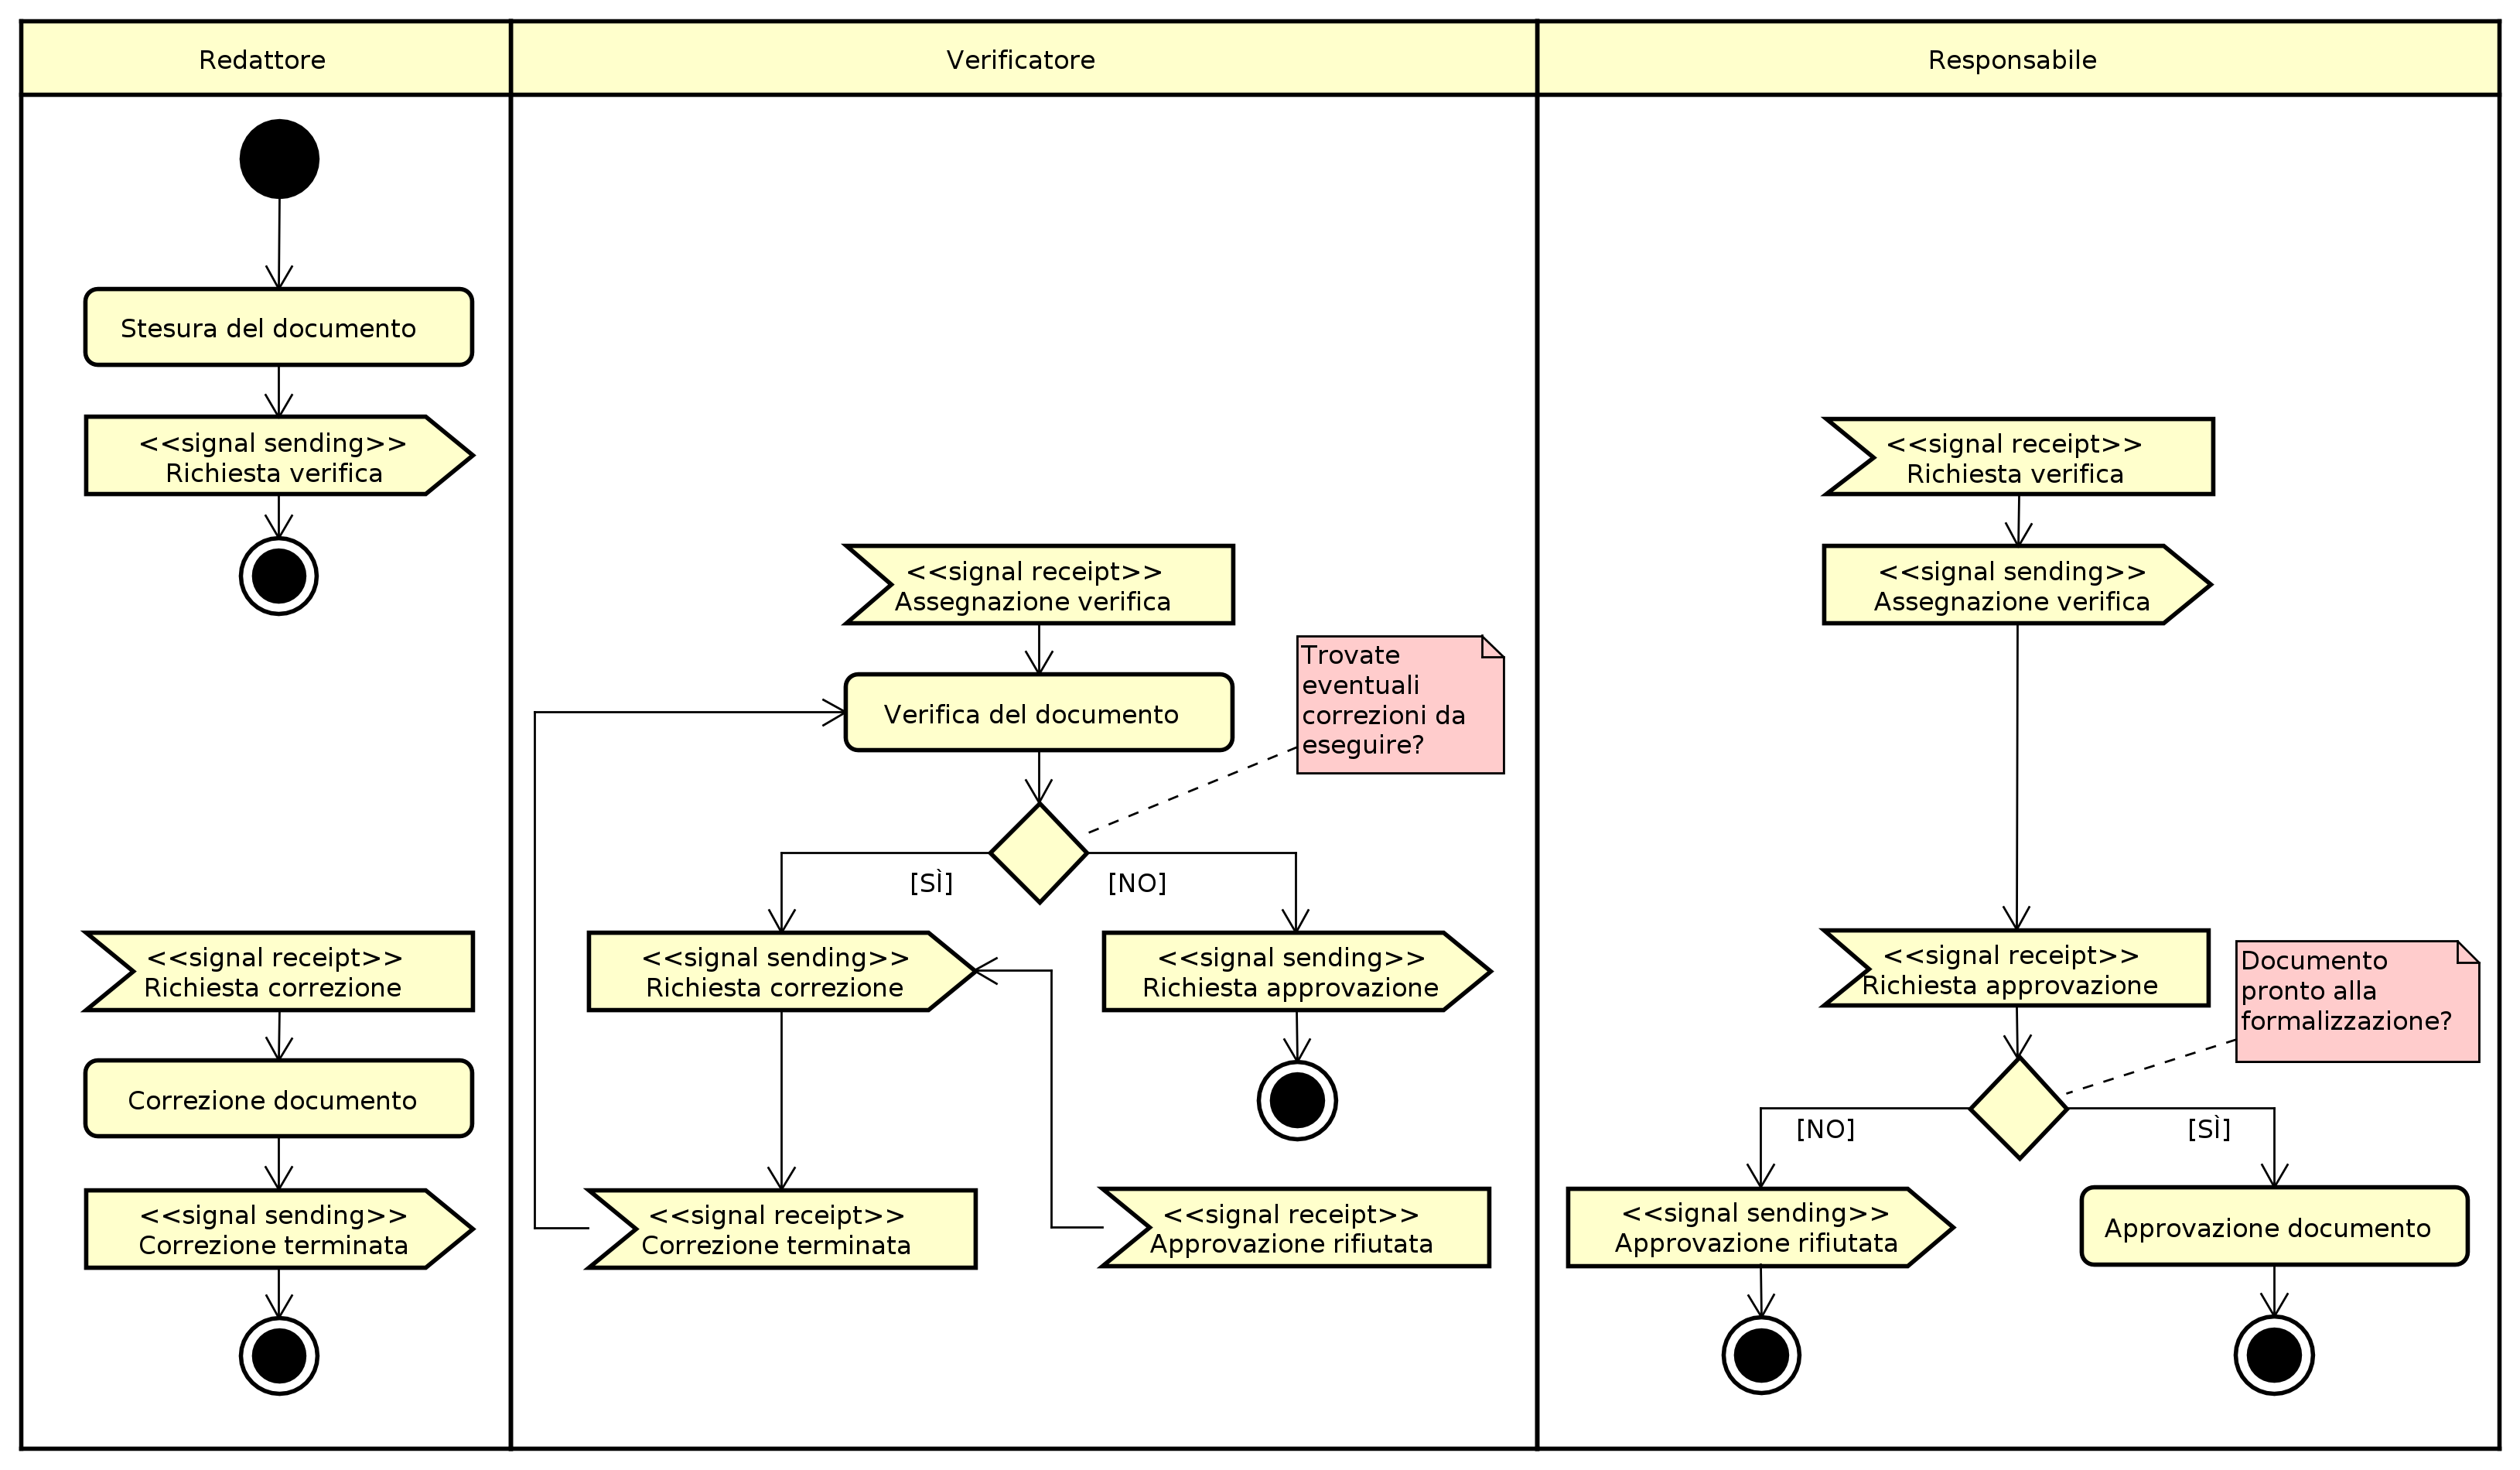
\includegraphics[width=\textwidth]{img/ciclo_di_vita_doc}
		        \caption{Ciclo di vita di un documento. Riferita nella sezione \ref{sec:ciclodivitadoc}}
                \label{fig:ciclovitadoc}
	        \end{figure}
	        
	        \paragraph{Aggiunta nuovi termini a glossario} \label{sec:insTermine}
	        Durante la stesura dei documenti, quando si ritiene che un termine debba essere inserito a glossario si deve seguire la seguente procedura:
	        \begin{enumerate}
	        	\item entrare nello spazio condiviso del gruppo su \glo{Google Drive}{Google Drive} (si veda sezione \ref{sec:GoogleDrive}) e aprire il foglio \texttt{Termini da inserire nel glossario};
	        	\item inserire il termine in fondo alla pagina.
	        \end{enumerate}
  
  \subsection{Gestione della configurazione}
  \subsubsection{Scopo}
        Lo scopo della gestione della configurazione è di individuare e gestire le parti che compongono i prodotti da realizzare (ovvero i Configuration Item, CI). La corretta implementazione del processo deve:
        \begin{itemize}
            \item individuare i CI;
            \item gestire la loro organizzazione all'interno del repository;
            \item gestire il versionamento.
        \end{itemize}

  \subsubsection{Repository}
  \paragraph{Struttura dei repository}
  Il gruppo ha scelto di utilizzare \glo{GitHub}{GitHub} per il versionamento e il salvataggio dei file inerenti le attività di progetto. L'\amministratore{} di progetto deve creare e organizzare i repository necessari e assicurarsi che tutti i membri del gruppo vi possano accedere. Ogni membro deve essere registrato su GitHub e aver attivato l'account studente.
  \newline \newline
  Il repository dedicato ai documenti si trova al seguente indirizzo:
  \begin{center}
  	\url{https://github.com/JordanGottardo/Documenti}
  \end{center}
  Il repository dedicato al codice si trova al seguente indirizzo:
  \begin{center}
  	\url{https://github.com/JordanGottardo/DeGeOp}
  \end{center}
  Le cartelle nel repository vengono organizzate nel seguente modo a partire dalla root:
  \begin{itemize}
  	\item \textbf{documenti:} sono presenti le cartelle per ogni revisione del progetto:
  	\begin{itemize}
  		\item \textbf{01-RR}: contenente i documenti e i file le necessari alla \revereq;
  		\item \textbf{02-RP}: contenente i documenti e i file le necessari alla \revprog;
  		\item \textbf{03-RQ}: contenente i documenti e i file le necessari alla \revaqual;
  		\item \textbf{04-RA}: contenente i documenti e i file le necessari alla \revacc;
  		\item \textbf{Script}: contenente script e altri strumenti utili per la stesura e la verifica dei documenti;
  		\item \textbf{Modello nuovo documento:} contenente i file con la struttura di base la creazione di un nuovo documento;
  		\item \textbf{Template}: contenente i file del template da usare per la creazione dei documenti \LaTeX.
  		\item \textbf{Consegne}: contenente i file delle consegne suddivise per revisione.
  	\end{itemize}
  	\item \textbf{codice}: la descrizione di questa cartella verrà fornita in un momento successivo.
  \end{itemize}
  
  \paragraph{Nomi dei file}
  I nomi dei documenti presenti nel repository devono rispettare la notazione \glo{Camel case}{camel case} con le seguenti caratteristiche:
  \begin{itemize}
  	\item la prima lettera di ogni file è maiuscola, le successive minuscole fino al presentarsi della parola successiva che inizia con la lettera maiuscola e cosi via;
  	\item è possibile utilizzare unicamente caratteri alfanumerici e il trattino basso;
  	\item i nomi non possono contenere spazi o elementi di punteggiatura.
  \end{itemize}

  \subsubsection{Versionamento}\label{sec:versionamento}
	  \paragraph{Controllo di versione}
	  Il controllo di versione del file sorgente, sia per il codice sia per i documenti, viene fatto utilizzando il software \glo{Git}{Git} e la piattaforma GitHub. 
	  \paragraph{Versionamento documenti}
		  Tutti i documenti devono essere identificati da una versione, ad ogni nuova versione deve corrispondere una riga nel registro delle modifiche.
		  La versione corrente di un documento deve sempre essere riportata all'interno dello stesso e va inoltre indicata in coda al nome del file con il seguente formato:\\\\
		  \centerline{\texttt{NomeDocumento\_vX.Y.Z.pdf}}
		  \begin{itemize}
		  	\item \textbf{X:}
		  	\begin{itemize}
		  		\item inizia da 0;
		  		\item viene incrementato solo dal \responsabilediprogetto, al momento della sua approvazione; 
		  		\item non può essere maggiore del numero di revisioni.
		  	\end{itemize}
		  	\item \textbf{Y:}
		  	\begin{itemize}
		  		\item inizia da 0;
		  		\item viene incrementato solo dai \verificatori{} ad ogni verifica eseguita;
		  		\item quando viene incrementato X, viene riportato a 0.
		  	\end{itemize}
		  	\item \textbf{Z:}
		  	\begin{itemize}
		  		\item inizia da 0;
		  		\item viene incrementato solo dai redattori al completamento di ogni task di modifica del documento;
		  		\item quando vengono incrementati X o Y, viene riportato a 0.
		  	\end{itemize}
		  \end{itemize}

		\paragraph{Versionamento applicazione}
		L'applicazione realizzata verrà versionata nel seguente modo:
		\begin{itemize}
			\item \textbf{X:}
			\begin{itemize}
				\item inizia da 0;
				\item viene incrementato solo dal \responsabilediprogetto, corrisponde all'ultima versione stabile del applicazione; 
				\item la versione 1 coinciderà con la revisione di accettazione.
			\end{itemize}
			\item \textbf{Y:}
			\begin{itemize}
				\item inizia da 0;
				\item viene incrementato solo dai \verificatori{} ad ogni incremento di funzionalità eseguito;
				\item quando viene incrementato X, viene riportato a 0.
			\end{itemize}
			\item \textbf{Z:}
			\begin{itemize}
				\item inizia da 0;
				\item viene incrementato solo dai \programmatori{} al completamento di ogni task di modifica;
				\item quando vengono incrementati X o Y, viene riportato a 0.
			\end{itemize}
		\end{itemize}
  
        \paragraph{Messaggi di commit}
        Ogni volta che si effettuano modifiche sui file del repository locale per poi esser caricate in quello remoto, bisogna specificarne le motivazioni. Per uniformare l'ambiente di lavoro è stato scelto un formato standard per la scrittura dei messaggi di \glo{Commit}{commit} che devono contenere:
        \begin{itemize}
            \item breve messaggio riassuntivo delle operazioni svolte;
            \item lista dei file modificati;
            \item lista delle modifiche per i singoli file.
        \end{itemize}
        Si veda la sezione \ref{sec:commit} per il dettaglio sulla procedura da seguire.
  
	  \subsubsection{Strumenti}
	  \paragraph{Git}
	  Git è un \glo{Sistema di controllo di versione}{sistema software di controllo di versione} distribuito e \glo{Open source}{open source}. La versione utilizzata al momento della stesura di questo documento è la 2.11.0 o superiore.
	  Le principali motivazioni che hanno portato il gruppo alla scelta di questo strumento sono:
	  \begin{itemize}
	  	\item ampio uso in ambito lavorativo;
	  	\item performance superiori rispetto ad altri sistemi di versionamento;
	  	\item sistema distribuito anziché centralizzato.
	  \end{itemize}
	  Indirizzo per il download e documentazione:
	  \begin{center}
	  	\url{https://git-scm.com}
	  \end{center}
	  L'utilizzo di Git verrà effettuato tramite riga di comando. Si lascia libertà ai membri del gruppo per l'installazione di eventuali interfacce grafiche personalizzate.
	  %
	  \paragraph{GitHub}
	  GitHub è un servizio web di hosting per lo sviluppo di progetti software. Tra le caratteristiche principali:
	  \begin{itemize}
	  	\item utilizzo del sistema di controllo di versione Git;
	  	\item possibilità di inserire documentazione e immagini, oltre al codice sorgente ;
	  	\item \glo{Issue}{issue} tracking;
	  	\item funzionalità simili ai social network come follower, commenti e notifiche;
	  	\item visione di grafici e statistiche su sviluppatori e repository.
	  \end{itemize}
	  Le principali motivazioni che hanno portato il gruppo alla scelta di questo strumento sono:
	  \begin{itemize}
	  	\item possibilità di creare repository private attivando il piano studente con l'email universitaria;
	  	\item sistema largamente diffuso e conosciuto da alcuni membri del gruppo;
	  	\item integrabile con altre applicazioni (es: \glo{Slack}{Slack}, \glo{IDE}{IDE}).
	  \end{itemize}
  
	  \subsubsection{Procedure}
	  \paragraph{Installazione e configurazione di Git}
	  L'installazione di Git varia a seconda del sistema operativo utilizzato. Di seguito verranno elencate le principali procedure d'installazione.
	  \newline \newline
	  Per i sistemi \glo{Linux}{Linux}:
	  \begin{itemize}
	  	\item aprire il terminale;
	  	\item eseguire il comando sudo \texttt{apt-get update};
	  	\item eseguire il comando \texttt{apt-get install git}.
	  \end{itemize}
	  Per i sistemi \glo{Windows}{Windows}:
	  \begin{itemize}
	  	\item accedere al sito ufficiale \url{https://git-scm.com/download/win};
	  	\item scaricare l'eseguibile;
	  	\item installare l'eseguibile seguendo la procedura guidata.
	  \end{itemize}
	  Per i sistemi \glo{MacOS}{MacOS}:
	  \begin{itemize}
	  	\item accedere al sito ufficiale \url{https://git-scm.com/download/mac};
	  	\item scaricare l'eseguibile;
	  	\item aprire il file appena scaricato e avviare l'installazione cliccando sul file \texttt{.pkg}.
	  \end{itemize}
	  La configurazione iniziale prevede l'inserimento del nome dell'utente e la connessione con l'account GitHub tramite la seguente procedura:
	  \begin{itemize}
	  	\item \texttt{{git} config --global user.name <Nome Cognome>}: imposta il nome dell'utente, che comparirà come autore delle commit effettuate;
	  	\item \texttt{{git} config --global user.email <email>}: imposta l'email dell'utente; deve essere impostata la stessa email utilizzata per la registrazione su GitHub.
	  \end{itemize}
	  Per la creazione di una cartella locale del repository si deve seguire la seguente procedura:
	  \begin{itemize}
	  	\item creare una nuova cartella;
	  	\item aprire il terminale;
	  	\item posizionarsi all'interno della cartella precedentemente creata;
	  	\item eseguire il comando: \texttt{git init};
	  	\item recuperare l'indirizzo URL del progetto su GitHub;
	  	\item eseguire il comando: \texttt{git clone <indirizzo appena recuperato>}.
	  \end{itemize}
	  \paragraph{Aggiornamento del repository} \label{sec:commit}
	  L'aggiornamento del repository deve essere svolto eseguendo i seguenti comandi:
	  \begin{enumerate}
	  	\item eseguire \texttt{git pull} per scaricare le modifiche da remoto;
	  	\item se sono presenti conflitti:
	  	\begin{enumerate}
	  		\item eseguire \texttt{git stash} per salvare momentaneamente le modifiche locali;
	  		\item eseguire \texttt{git pull};
	  		\item eseguire \texttt{git stash apply} per ripristinare le modifiche;
	  	\end{enumerate}
	  	\item eseguire \texttt{git add NomeFile} per ognuno dei file in cui sono state effettuate delle modifiche;
	  	\item eseguire \texttt{git commit -m "descrizione modifiche"};
	  	\item eseguire \texttt{git push} per inviare le modifiche al repository remoto.
	  \end{enumerate}
	  \begin{figure}[H]
	  	\centering
	  	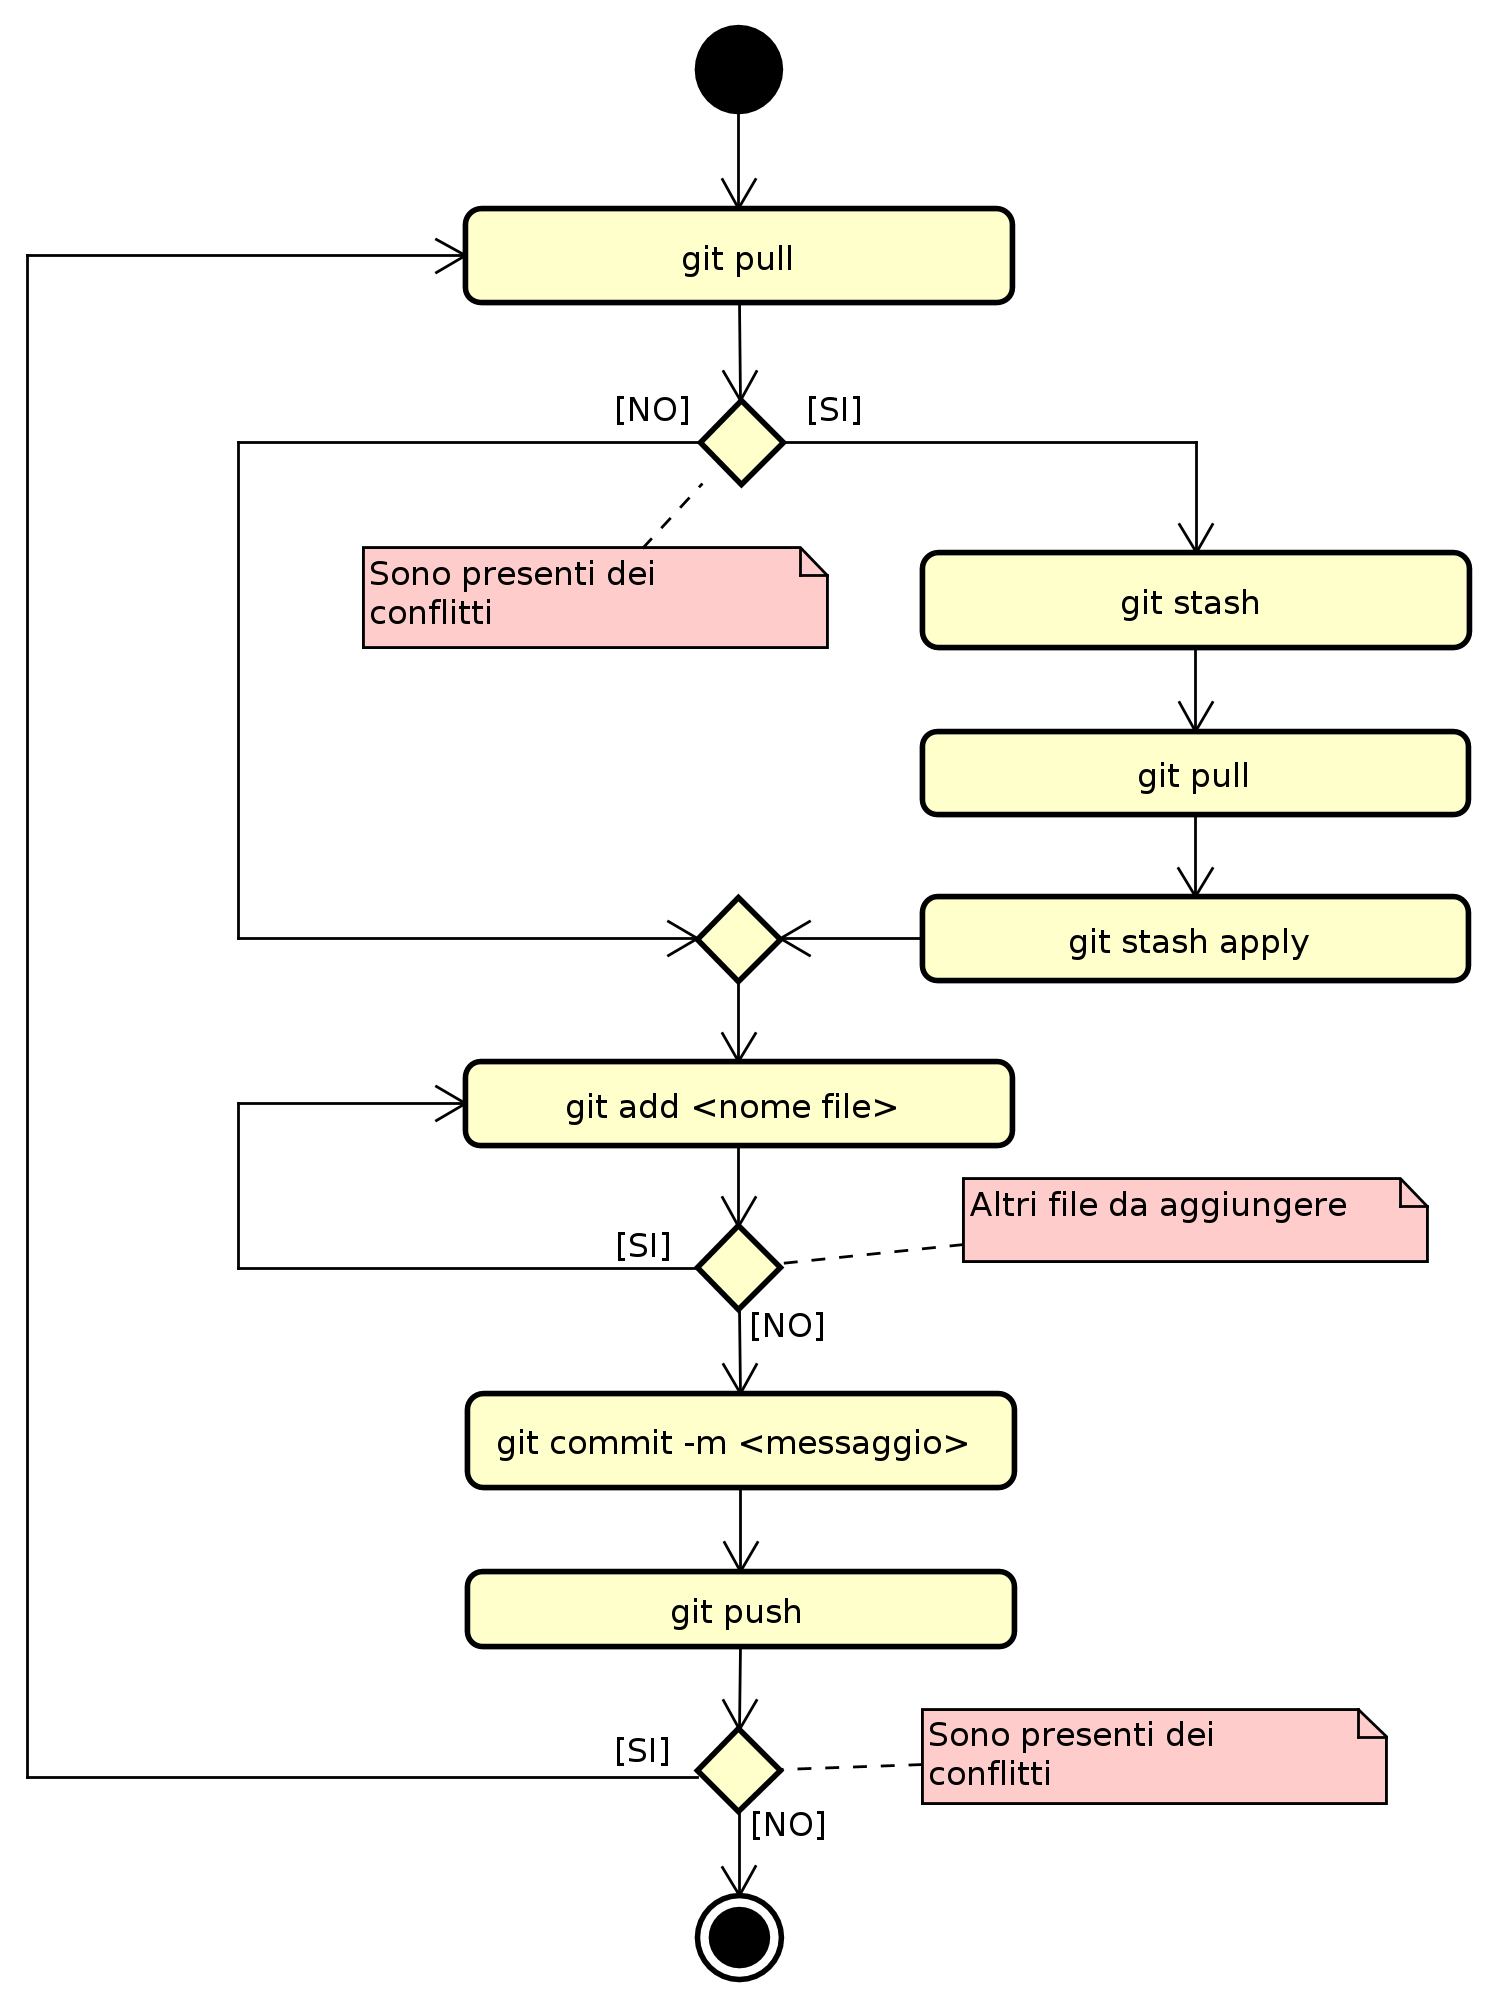
\includegraphics[width=0.7\textwidth]{img/AggiornamentoRepository}
	  	\caption{Procedura di aggiornamento del repository.}
	  \end{figure}
	  \paragraph{Comandi utili Git}
	  Per l'approfondimento dei principali comandi riguardanti l'utilizzo di Git è stata redatta una guida, consultabile al seguente indirizzo: \href{https://github.com/JordanGottardo/Documenti/blob/master/README.md}{Guida Git}.
	%
	
    \subsection{Verifica}\label{sec:verifica}
        \subsubsection{Scopo}
        Lo scopo del processo di verifica è di garantire che ogni attività dei processi svolti non introduca errori nel prodotto e che soddisfi i requisiti o le condizioni necessarie per essere considerata accettabile. La corretta implementazione del processo deve:
        \begin{itemize}
            \item fornire le procedure di verifica necessarie;
            \item individuare i criteri per la verifica;
            \item individuare eventuali difetti perchè possano essere corretti.
        \end{itemize}
		\subsubsection{Documenti} \label{sec:documenti}
		Il \responsabilediprogetto{} deve assegnare i compiti ai \verificatori, ognuno di essi deve effettuare un controllo accurato delle seguenti regole:
		\begin{itemize}
			\item devono essere rispettate le norme tipografiche (vedi sez. \ref{sec:normeTipografiche});
			\item devono essere rispettate le componenti grafiche (vedi sez. \ref{sec:normeGrafiche});
			\item devono essere rispettate le regole per i termini a glossario (vedi sez. \ref{sec:normeGlossario});
			\item devono essere utilizzati periodi brevi, corretti e il più possibile semplici;
			\item devono essere usati i comandi \LaTeX{} descritti nell'appendice \ref{ComandiLatex};
			\item deve essere rispettata la struttura del documento (vedi sez. \ref{sec:strutturaDoc}).
		\end{itemize}
	
		\subsubsection{Metriche}
			\paragraph{Processi}
				\subparagraph{Livello CMM ($LCMM$)} \label{LCMM}
				La metrica scelta è il Livello \glo{CMM}{CMM} (LCMM). La scala assume valori da 1 (peggiore) a 5 (migliore).
				%
				\subparagraph{Schedule Variance ($SV$)} \label{SV}
				La metrica utilizzata è la Schedule Variance (SV). È implementata come differenza tra la pianificazione dei costi del lavoro eseguito e del lavoro pianificato. Entrambi questi valori sono intesi nella loro accezione temporale (giorni) e non monetaria.
				$$SV = BCWP-BCWS$$
				dove $BCWP$=Budgeted Cost of Work Performed e $BCWS$=Budgeted Cost of Work Scheduled.
				%
				\subparagraph{Cost Variance ($CV$)} \label{CV}
				La metrica utilizzata è la Cost Variance (CV). È implementata come differenza tra costo pianificato e costo effettivo del lavoro eseguito.
				$$CV = BCWP-ACWP$$ dove $BCWP$=Budgeted Cost of Work Performed e $ACWP$=Actual Cost of Work Performed.
				%
				\subparagraph{Rischi Non Preventivati ($RNP$)} \label{RNP}
				È stato creato un contatore RNP (Rischi Non Preventivati) che aumenta di 1 ogni volta che si presenta un rischio non preventivato nel \pdpv. Il contatore rimane attivo durante tutto il ciclo di vita del progetto.
				%
				\subparagraph{Righe Documento Per Ora ($RDCO$)} \label{RDCO}
				È stato creato un contatore RDCO (Righe Documento Per Ora) che tiene conto delle righe di documento che vengono redatte da un membro del gruppo.
				$$RDCO=\frac{RP}{OI}$$ dove $RP$=Righe Prodotte e $OI$=Ore Impiegate nella scrittura del documento
				%
				\subparagraph{Numero Comandi Richiesti ($NCR$)} \label{NCR}
				È stato creato un contatore NCR (Numero Comandi Richiesti) che tiene conto dei comandi personalizzati per il template \LaTeX{} che vengono richiesti al \responsabilediprogetto.
				%
				\subparagraph{Risoluzione Verticale ($RV$)} \label{RV}
				Metrica che tiene conto dei pixel verticali di un'immagine.
				Come riferimento viene preso il valore di $RV$ minimo tra le immagini.
				%
				\subparagraph{Percentuale Tracciamento Modifiche ($PTM$)} \label{PTM}
				$$PTM=\frac{NTC}{NARM}$$
				dove $NTC$=Numero di Task Completati relativi ad un documento e $NARM$=Numero Aggiunte Registro Modifiche.
				%
				\subparagraph{Righe Codice Per Ora ($RCPO$)} \label{RCPO}
				$$RCPO=\frac{RC}{OI}$$
				dove $RC$=Righe di Codice scritte e $OI$=Ore Impiegate.
				%
				\subparagraph{Use Case senza Scenario Principale ($UCSP$)} \label{UCSP}
				Metrica che tiene conto del numero di use case senza scenario principale.
				%
				\subparagraph{Percentuale di Requisiti Obbligatori Coperti ($PROC$)} \label{PROC}
				$$PROC=\frac{ROC}{ROI}$$
				dove $ROC$=Requisiti Obbligatori Coperti, ovvero assegnati ad un \glo{Package}{package} e $ROI$=Requisiti Obbligatori Individuati.
				%
				\subparagraph{Grado di Accoppiamento ($GA$)} \label{GA}
				Metrica che indica le dipendenze uscenti delle componenti (package/classi) del sistema verso altre componenti. 
				Viene preso come riferimento il massimo $GA$ tra quelli presenti.
				%
				\subparagraph{Grado di Utilità ($GU$)} \label{GU}
				Metrica che indica le dipendenze entranti nelle componenti del sistema.
				Viene preso come riferimento il minimo $GU$ tra quelli presenti.
				%
			\paragraph{Documenti}
				\subparagraph{Indice Gulpease ($IG$)} \label{IG}
				La metrica utilizzata è l'\glo{Indice Gulpease}{Indice Gulpease} ($IG$), un indice di leggibilità di un testo tarato sulla lingua italiana. La scala va da 0 a 100, dove "0" indica un documento di bassa leggibilità e "100" uno di alta. Risulta che i testi con indice:
				\begin{itemize}
					\item inferiore a 80 sono difficili da leggere per chi ha la licenza elementare;
					\item inferiore a 60 sono difficili da leggere per chi ha la licenza media;
					\item inferiore a 40 sono difficili da leggere per chi ha un diploma superiore.
				\end{itemize}
				$$IG=89 + \frac{300\cdot{}NF-10\cdot{}NL}{NP}$$
				dove $NF$ è il Numero di Frasi, $NL$ è il Numero di Lettere e $NP$ è il Numero di Parole presenti nel testo.
				%
				\subparagraph{Errori riguardanti le Norme interne e Non Corretti ($ENNC$)} \label{ENNC}
				La metrica utilizzata è il numero di Errori riguardanti le Norme interne rinvenuti e Non Corretti ($ENNC$). È implementata con un contatore che aumenta di 1 ogni volta che un errore riguardante le norme interne rilevato da un \verificatore{} non viene corretto. Il contatore fa riferimento ad uno specifico \glo{Periodo}{periodo} e viene azzerato successivamente.
				%
				\subparagraph{Errori Ortografici Non Corretti ($EONC$)} \label{EONC}
				La metrica utilizzata è un contatore di Errori Ortografici Non Corretti ($EONC$), che aumenta di 1 ogni volta che un errore ortografico rilevato da un \verificatore{} non viene corretto. Il contatore fa riferimento ad uno specifico periodo e viene azzerato successivamente.
				%
				\subparagraph{Errori Concettuali Non Corretti ($ECNC$)} \label{ECNC}
				La metrica utilizzata è chiamata Errori Concettuali Non Corretti ($ECNC$). La formula è data dal complemento a 1 del rapporto tra errori concettuali corretti e rilevati. Tali errori possono essere rilevati dai Verificatori o dal committente.
				$$ECNC=\left(1-\frac{ECC}{ECR}\right)\cdot100$$
				dove $ECC$=Errori Concettuali Corretti e $ECR$=Errori Concettuali Rinvenuti.
				%
				\subparagraph{Livello Annidamento Indice ($LAI$)} \label{LAI}
				Metrica che conta il livello di annidamento dell’indice.
				Viene preso come riferimento il massimo $LAI$ tra quelli presenti.
				
			\paragraph{Codice}
				\subparagraph{Implementazione delle Funzionalità Obbligatorie ($IFO$)} \label{IFO}
				La metrica utilizzata è chiamata Implementazione delle Funzionalità Obbligatorie ($IFO$). Essa consiste in un rapporto tra il numero di requisiti obbligatori soddisfatti e identificati
				$$IFO= \frac{ROS}{ROI}\cdot 100$$
				dove $ROS$=numero di Requisiti Obbligatori Soddisfatti e $ROI$=numero di Requisiti Obbligatori Identificati.
				%
				\subparagraph{Implementazione delle Funzionalità Desiderabili ($IFD$)} \label{IFD}
				La metrica utilizzata è chiamata Implementazione delle Funzionalità Desiderabili ($IFD$). Essa consiste in un rapporto tra il numero di requisiti desiderabili soddisfatti e identificati
				$$IFD= \frac{RDS}{RDI}\cdot 100$$
				dove $RDS$=numero di Requisiti Desiderabili Soddisfatti e $RDI$=numero di Requisiti Desiderabili Identificati.
				%
				\subparagraph{Numero di Statement per Metodo ($NSM$)} \label{NSM}
				Metrica che conta il Numero di \glo{Statement}{Statement} per Metodo.
				Viene preso come riferimento il massimo $NSM$ tra quelli presenti.
				%
				\subparagraph{Numero di Parametri per Metodo ($NPM$)} \label{NPM}
				Metrica che conta il Numero di Parametri per Metodo.
				Viene preso come riferimento il massimo $NPM$ tra quelli presenti.
				%
				\subparagraph{Numero Campi Dati Per Classe ($NCDPC$)} \label{NCDPC}
				Metrica che conta il Numero di Campi Dati per Classe.
				Viene preso come riferimento il massimo $NCDPC$ tra quelli presenti.
				%
				\subparagraph{Numero Ciclomatico ($NC$)} \label{NC}
				La metrica è basata sul Numero Ciclomatico ($NC$). Il conteggio viene fatto a livello di metodo.
				$$NC=e-n+2p$$
				dove $e$=numero di archi, $n$=numero di nodi, $p$=numero di componenti connesse.\\
				Viene preso come riferimento il massimo $NC$ tra quelli presenti.
				%
				\subparagraph{Numero di Variabili dichiarate e Non Utilizzate ($NVNU$)} \label{NVNU}
				Metrica che conta il numero di variabili dichiarate e non utilizzate.
				%
				\subparagraph{Rapporto tra le linee di Commento e le linee di Codice ($RCC$)} \label{RCC}
				La metrica è implementata come Rapporto tra le linee di Commento e le linee di Codice ($RCC$).
				$$RCC=\left(\frac{LDCM}{LDCC}\right)\cdot 100$$
				dove $LDCC$=Linee Di Codice e $LDCM$=Linee Di Commento.
				%
				\subparagraph{Superamento dei Test Pianificati ($STP$)} \label{STP}
				La metrica utilizzata è il Superamento dei Test Pianificati ($STP$). I test presi in considerazione sono quelli necessari a verificare l'implementazione delle funzionalità previste dai requisiti.
				$$STP=\frac{TS}{TP}\cdot100$$
				dove $TS$=numero di Test Superati e $TP$=numero di Test Pianificati.
				%
				\subparagraph{Breakdown Avoidance ($BA$)} \label{BA}
				La metrica utilizzata è la Breakdown Avoidance ($BA$).
				$$BA=\left( 1-\frac{NI}{NSA} \right)\cdot 100$$
				dove $NI$=Numero di Interruzioni e $NSA$=Numero di Situazioni Anomale.
				%
				\subparagraph{Failure Avoidance ($FA$)} \label{FA}
				La metrica utilizzata è la Failure Avoidance ($FA$).
				$$FA=\left(\frac{SAE}{SAT}\right) \cdot 100$$
				dove $SAE$=Situazioni Anomale Evitate e $SAT$=Situazioni Anomale Testate.
				%
				\subparagraph{Statement Coverage ($SC$)} \label{SC}
				Metrica utilizzata per calcolare la copertura degli statement.
				$$SC=\frac{NSE}{NSM}$$
				dove $NSM$=Numero Statement del Metodo e $NSE$=Numero Statement Eseguiti dal test.
				Viene preso come riferimento il minimo $SC$ tra quelli presenti.
				%
				\subparagraph{Branch Coverage ($BC$)} \label{BC}
				Metrica utilizzata per calcolare la copertura dei flussi logici.
				$$BC=\frac{NFLT}{NFLM}$$
				dove $NFLT$=Numero di Flussi Logici del Metodo Testati e $NFLM$=Numero di Flussi Logici del Metodo.
				Viene preso come riferimento il minimo $BC$ tra quelli presenti.
		
		%\subsubsection{Test}
		
		\subsubsection{Strumenti}
		\paragraph{Tabella metriche processo-strumenti}
		\begin{table}[H]
			\centering
			\label{tab:metriceProcStrumenti}
			\begin{tabular}{cl}
				\toprule
				Metrica & Strumento \\
				\hline
				\hyperref[LCMM]{LCMM}    &  Procedura interna \ref{sec:lcmm} \\
				\hyperref[SV]{SV}      & \glo{Teamwork}{Teamwork}, vedi la sezione \ref{sec:procTicket}  \\
				\hyperref[CV]{CV}      & Teamwork, vedi sezione \ref{sec:procTicket}\\
				\hyperref[RNP]{RNP}     & Procedura interna \ref{sec:rnp} \\
				\hyperref[RDCO]{RDCO}    & Script interno, vedi procedura \ref{sec:loc} \\
				\hyperref[NCR]{NCR}     & Procedura interna \ref{sec:procRichieste} \\ 
				\hyperref[RV]{RV}      & Script interno, vedi procedura \ref{sec:imageRes} \\
				\hyperref[PTM]{PTM}     & Procedura interna \ref{sec:chiusuraticket}          \\
				\hyperref[RCPO]{RCPO}    & Script interno, vedi procedura \ref{sec:loc} \\ 
				\hyperref[UCSP]{UCSP}    & Statistiche \hyperref[sec:trender]{Trender} \\
				\hyperref[PROC]{PROC}    & Statistiche Trender \\
				\hyperref[GA]{GA} 		& Statistiche Trender \\
				\hyperref[GU]{GU}      & Statistiche Trender \\
				\bottomrule    
			\end{tabular}
			\caption{Tabella metriche processo-strumenti}
		\end{table}
		%
		\paragraph{Tabella metriche documenti-strumenti}
		\begin{table}[H]
			\centering
			\label{tab:metriceDocStrumenti}
			\begin{tabular}{cl}
				\toprule
				Metrica & Strumento \\
				\hline
				\hyperref[IG]{IG}    &  Script interno, vedi procedura \ref{sec:calcoloGulpease} \\
				\hyperref[ENNC]{ENCC} & Procedura interna \ref{sec:gestioneanomalie} \\
				\hyperref[EONC]{EONC} & Procedura interna \ref{sec:gestioneanomalie} \\
				\hyperref[ECNC]{ECNC} & Procedura interna \ref{sec:gestioneanomalie} \\
				\hyperref[LAI]{LAI} & Script interno, vedi procedura \ref{sec:ssPar} \\
				\bottomrule    
			\end{tabular}
			\caption{Tabella metriche documenti-strumenti}
		\end{table}
		%
		\paragraph{Tabella metriche codice-strumenti}
		\begin{table}[H]
			\centering
			\label{tab:metriceCodiceStrumenti}
			\begin{tabular}{cl}
				\toprule
				Metrica & Strumento \\
				\hline
				\hyperref[IFO]{IFO}		& Statistiche \hyperref[sec:trender]{Trender} \\
				\hyperref[IFD]{IFD}		& Statistiche Trender \\
				\hyperref[NSM]{NSM}		& \hyperref[sec:JSMeter]{JSMeter} \\
				\hyperref[NPM]{NPM}		& \hyperref[sec:ESLint]{ESLint} \\
				\hyperref[NCDPC]{NCDPC}	& Statistiche Trender \\
				\hyperref[NC]{NC}		& JSMeter \\
				\hyperref[NVNU]{NVNU} 	& ESLint \\
				\hyperref[RCC]{RCC}		& \hyperref[JSMeter]{JSMeter} \\
				\hyperref[STP]{STP}		& Statistiche \hyperref[par:trender]{Trender} \\
				\hyperref[BA]{BA}		& \hyperref[sec:Jasmine]{Jasmine} \\
				\hyperref[FA]{FA}		& Jasmine \\
				\hyperref[SC]{SC}		& \hyperref[sec:WebStorm]{WebStorm} tramite \hyperref[sec:Karma]{Karma} e \hyperref[sec:Istanbul]{Istanbul} \\
				\hyperref[BC]{BC}		& WebStorm tramite Karma e Istanbul \\
				\bottomrule    
			\end{tabular}
			\caption{Tabella metriche codice-strumenti}
		\end{table}
		\paragraph{Verifica ortografica}
		Viene utilizzato il correttore in tempo reale integrato nell'applicazione \glo{TeXstudio}{TeXstudio} descritta nella sezione \ref{sec:texstudio}. Il correttore identifica e sottolinea eventuali refusi ortografici; un'analisi più approfondita del testo è compito dei \verificatori.
		%
		\paragraph{Indice leggibilità} \label{sec:gulpease}
		La valutazione dell'indice di leggibilità è fatta secondo l'\glo{Indice Gulpease}{indice Gulpease} utilizzando uno script creato appositamente e fornito assieme al template. Lo script può analizzare sia il file sorgente scritto in \TeX{} che il file pdf risultante.
		%
		\paragraph{Analisi statica}
		\subparagraph{ESLint} \label{sec:ESLint}
		ESLint è un tool che permette di effettuare analisi statica su file \glo{JavaScript}{JavaScript} con lo scopo di ottenere codice più uniforme e privo di errori. I controlli che effettua sul codice vengono realizzati nei confronti di un insieme di regole personalizzabili, regole che gli sviluppatori possono attivare o disattivare in base alle loro guide di stile di codifica interna (vedi sezione: \ref{sec:stileCodifica}). \\
		La documentazione e l'installazione di ESLint sono disponibili al seguente indirizzo:
		\begin{center}
			\url{https://github.com/eslint/eslint}
		\end{center}
		%
		\subparagraph{JSMeter} \label{sec:JSMeter}
		JSMeter è uno strumento che permette di calcolare diversi indici di misurazione della complessità del codice JavaScript descritti nel \pdqv.
		La documentazione e l'installazione di JSMeter sono disponibili al seguente indirizzo:
		\begin{center}
			\url{http://jsmeter.info}
		\end{center}
		%
		\paragraph{Analisi dinamica}
		\subparagraph{Karma}\label{sec:Karma}
		Karma è un ambiente di testing, utile ad effettuare test su browser e dispositivi. Per descrivere i test vengono utilizzati dei framework esterni, come per esempio Mocha o Jasmine. Karma viene utilizzato assieme ad un framework per l'esecuzione dei test di unità. \\
		La documentazione e l'installazione di Karma sono disponibili al seguente indirizzo:
		\begin{center}
			\url{https://github.com/karma-runner/karma}
		\end{center}
		%
		\subparagraph{Jasmine}\label{sec:Jasmine}
		\glo{Jasmine}{Jasmine} è un framework per implementare test di codice \js, non dipendendo da browser o altri framework è adatto ad eseguire test di siti web ed è facilmente estendibile. Oltre a mettere a disposizione un set di operazioni di confronto permette anche di utilizzare driver e stub. I test implementati possono essere eseguiti tramite l'inserimento del codice in uno specifico file html o utilizzando un test runner esterno come Karma.
		La documentazione e l'installazione di Jasmine sono disponibili al seguente indirizzo:
		\begin{center}
			\url{https://jasmine.github.io/index.html}
		\end{center}
		%
		\subparagraph{Istanbul}\label{sec:Istanbul}
		Instanbul è uno strumento che permette di calcolare alcune metriche di complessità del codice JavaScript descritte nel \pdqv{} e verrà installato come modulo per \glo{Node.js}{Node.js}.
		La documentazione e l'installazione di Istanbul sono disponibili al seguente indirizzo:
		\begin{center}
			\url{https://github.com/gotwarlost/istanbul}
		\end{center}
		%
		%		        \subparagraph{Mocha}
		%		        Mocha è un framework per l’esecuzione di test JavaScript; permette l'esecuzione di test asincroni ed in serie, consentendo segnalazioni flessibili ed accurate.\\
		%		        La documentazione e l'installazione di Mocha è raggiungibile al seguente indirizzo:
		%		        \begin{center}
		%		        	\url{https://github.com/mochajs/mocha}
		%		        \end{center}
		%		        %
		%		        \subparagraph{Enzyme}
		%		        Enzyme è un tool di testing JavaScript per React che permette di testare facilmente il DOM; va abbinato alla libreria Chai.\\
		%		        La documentazione e l'installazione di Enzyme è raggiungibile al seguente indirizzo:
		%		        \begin{center}
		%		        	\url{https://github.com/airbnb/enzyme/}
		%		        \end{center}
		%		        %
		%		        \subparagraph{Chai}
		%		        Chai è una libreria per gestire le asserzioni. Viene utilizzata assieme a molti framework di test per JavaScript.\\
		%		        La documentazione e l'installazione di Chai sono disponibili al seguente indirizzo:
		%		        \begin{center}
		%		        	\url{https://github.com/chaijs/chai}
		%		        \end{center}
		%		        %
		%		        \subparagraph{Sinon}
		%		        Sinon è un framework che fornisce spie, stub e mock per creare e svolgere i test di unità.
		%		        La documentazione e l'installazione di Sinon sono disponibili al seguente indirizzo:
		%		        \begin{center}
		%		        	\url{https://github.com/sinonjs/sinon}
		%		        \end{center}
		
        \subsubsection{Procedure}
	        \paragraph{Attività manuale di verifica}
	        Ogni attività manuale di verifica deve essere accompagnata da un resoconto (si veda la sez. \ref{sec:gestioneanomalie} per i dettagli). Per svolgere l'attività di verifica, il \verificatore{} deve rispettare le seguenti indicazioni:
	        \begin{enumerate}
	        	\item aprire il file sorgente da verificare (se è un documento, anche il file pdf);
	        	\item annotare gli errori rilevati da correggere;
	        	\item inserire nel codice sorgente uno dei seguenti commenti:
		        	\begin{itemize}
		        		\item TODO per segnalare un'aggiunta da eseguire al codice;
		        		\item FIXME per segnalare un errore rilevato per cui è stata proposta una soluzione;
		        		\item BUG per segnalare un'anomalia da rivedere e correggere;
		        	\end{itemize} 
	        	\item se è un documento, calcolare indice gulpease (vedi sez. \ref{sec:gulpease}) e riportare l'esito nel resoconto;
	        	\item aprire un subticket come riportato nella sez. \ref{sec:gestioneanomalie} riportando gli errori.
	        \end{enumerate}
    
            \paragraph{Analisi}
                \subparagraph{Analisi statica}
                Tecnica utilizzata per l'analisi e la verifica del codice sorgente e della documentazione associata. Può essere applicata secondo due strategie:
                \begin{itemize}
                    \item \textbf{\glo{Walkthrough}{walkthrough}:} lettura completa del codice sorgente da analizzare. Va utilizzata unicamente durante il primo periodo del progetto in quanto risulta onerosa e non efficiente. Gli \analisti{} che la utilizzano devono stilare una lista di controllo con gli errori rilevati più frequentemente;
                    \item \textbf{\glo{Inspection}{inspection}:} lettura mirata del codice sorgente da analizzare. È necessario avere una lista di controllo per poter localizzare eventuali punti critici in cui cercare errori. Dopo ogni analisi la lista di controllo deve essere incrementata con eventuali nuovi errori rilevati.
                \end{itemize}
                \subparagraph{Analisi dinamica}
                Tecnica per l'analisi del prodotto software, richiede l'esecuzione del programma e viene eseguita tramite dei test che verificano il funzionamento del prodotto. I test devono essere ripetibili e a parità di condizioni iniziale e ambiente devono fornire lo stesso output. Per ogni test deve quindi essere definito:
                \begin{itemize}
                    \item \textbf{ambiente:} sistema hardware e software in cui viene eseguito il test;
                    \item \textbf{stato iniziale:} stato iniziale da cui si parte ad eseguire il test;
                    \item \textbf{input:} input inserito;
                    \item \textbf{output:} output atteso.
                \end{itemize}
            
            \paragraph{Task di verifica}\label{sec:taskverifica}
            La gestione dei task di verifica avviene tramite la creazione di ticket nell'applicazione \glo{Teamwork}{Teamwork} che viene descritta nella sezione \ref{sec:teamwork}. \\
	        Al termine di ogni ticket il \responsabilediprogetto{} dovrà seguire la seguente procedura:
            \begin{enumerate}
                \item creare un ticket di verifica con i riferimenti al task da verificare e contrassegnarlo con la dicitura \cit{[VERIFICA]};
                \item assegnare il ticket creato ad un \verificatore;
                \item al completamento del ticket di verifica contrassegnare il ticket originale con la dicitura \cit{[VERIFICATO]}.
            \end{enumerate}
            Vedi anche figura \ref{fig:verificagestione}. \\

            \paragraph{Gestione delle anomalie}\label{sec:gestioneanomalie}
            La gestione delle anomalie durante il processo di verifica avviene tramite la creazione di ticket nell'applicazione Teamwork che viene descritta nella sezione \ref{sec:teamwork}. Nel caso in cui un \verificatore{} dovesse trovare delle anomalie durante un task di verifica queste dovranno essere gestite nel seguente modo:
            \begin{enumerate}
                \item deve essere creato un subticket contrassegnato da uno dei seguenti tag, questi saranno utilizzati in un secondo momento per il calcolo delle relative metriche:
                \begin{itemize}
                	\item \cit{[EN]} se l'anomalia riguarda il rispetto delle norme (vedi metrica \ref{ENNC});
                	\item \cit{[EO]} se l'anomalia riguarda un errore ortografico (vedi metrica \ref{EONC});
                	\item \cit{[EC]} se l'anomalia riguarda un errore concettuale (vedi metrica \ref{ECNC});
                	\item \cit{[ERR]} se l'anomalia non riguarda nessuno dei campi precedenti.
                \end{itemize}
                \item assegnare i subticket creati agli assegnatari del task di cui si sta eseguendo la verifica;
                \item al completamento di tutti i subticket chiudere il ticket di verifica.
            \end{enumerate}
            Vedi anche figura \ref{fig:verificagestione}.

            \begin{figure}[H]
		        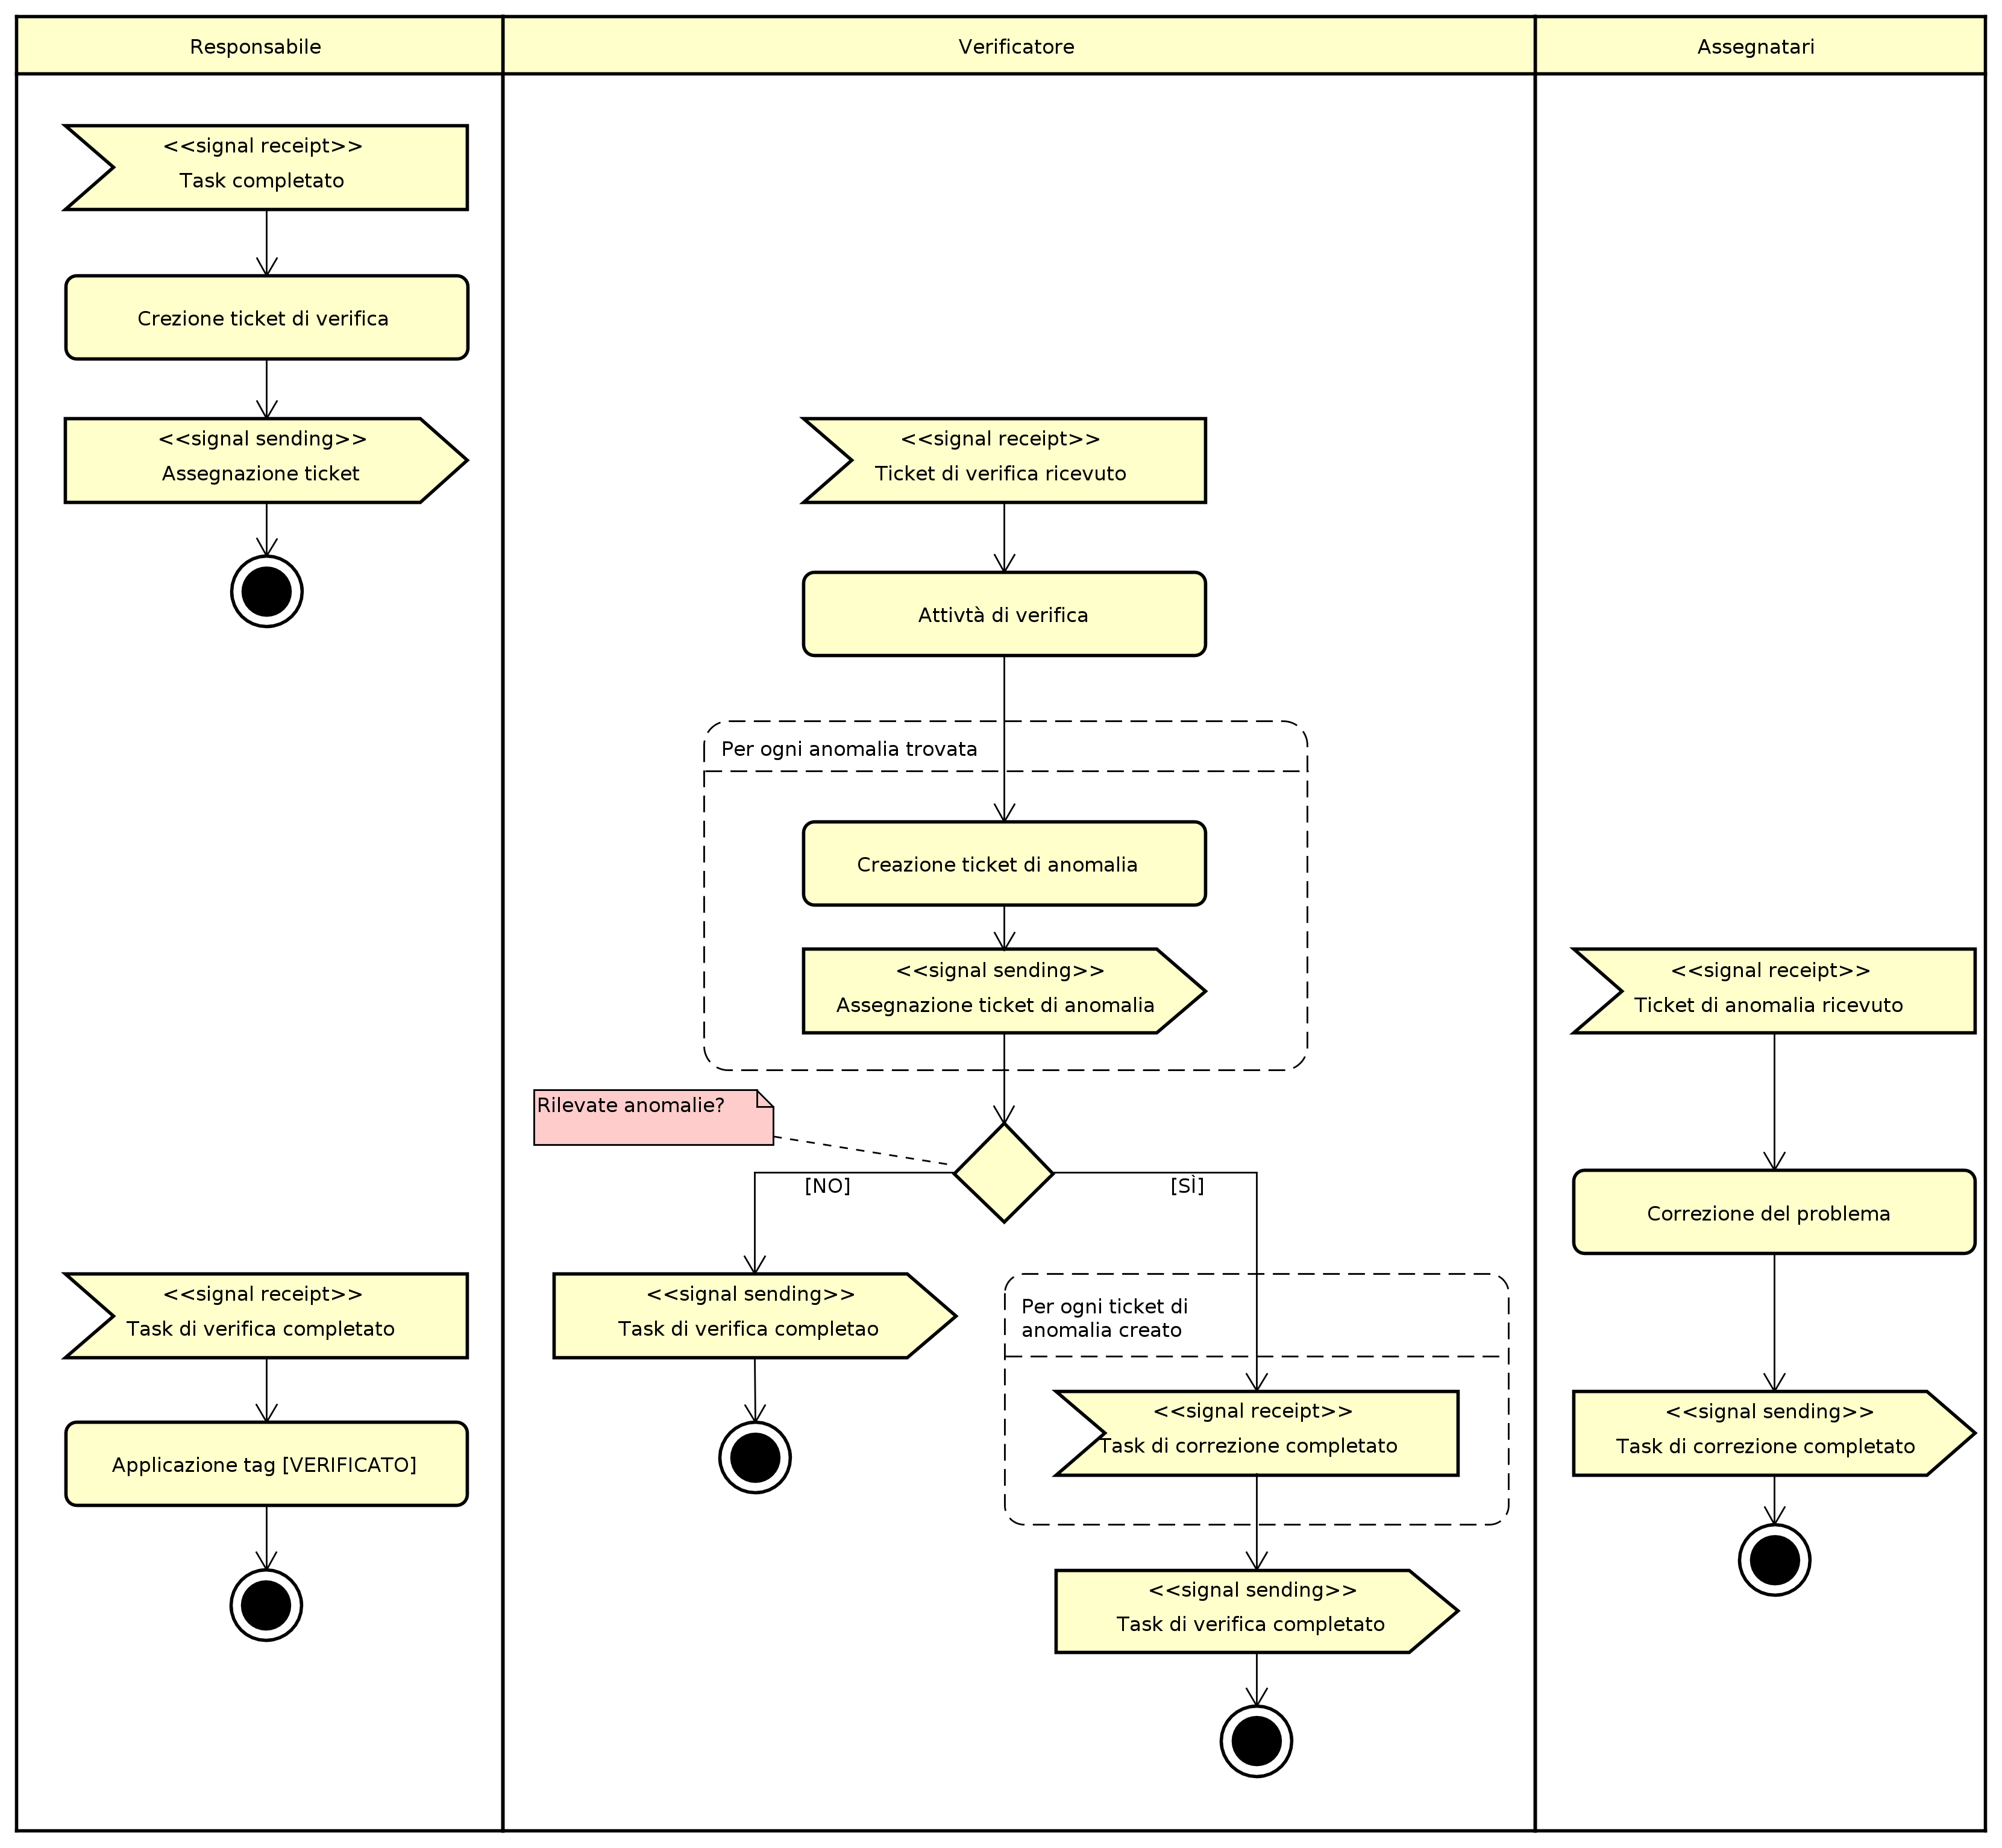
\includegraphics[width=\textwidth]{img/verifica_gestione_task}
		        \caption{Procedura di verifica dei task e gestione delle anomalie. Riferita nelle sezioni \ref{sec:taskverifica} e \ref{sec:gestioneanomalie}}
                \label{fig:verificagestione}
	        \end{figure}
	        %
	        \paragraph{Calcolo CMM}\label{sec:lcmm}
	        Al termine di ogni periodo il \responsabilediprogetto{} ha il compito di individuare il livello CMM che si è raggiunto. La decisione deve essere presa tenendo in considerazione:
	        \begin{itemize}
	        	\item le norme prodotte fino a quel momento ed il loro rispetto;
	        	\item i processi svolti, i loro risultati e la loro riproducibilità;
	        	\item le metriche individuate ed i loro valori.
	        \end{itemize} 
	        %
	        \paragraph{Calcolo rischi non preventivati}\label{sec:rnp}
	        Al momento di attualizzare un rischio il \responsabilediprogetto{} deve verificare che tale rischio sia presente nel \pdp{}. Se così non fosse dovrà procedere nel seguente modo:
	        \begin{itemize}
	        	\item creare un task ed inserire nel titolo il tag \cit{[RISK]};
	        	\item scrivere nella descrizione del task il rischio riscontrato;
	        	\item assegnare il task ad un analista responsabile del \pdp{} in modo che sia inserito nel documento.
	        \end{itemize}
	        Il \responsabilediprogetto{} dovrà tenere traccia dei ticket creati con il tag \cit{[RISK]} per calcolare il valore della metrica.
	        %
	        \paragraph{Calcolo dell'indice Gulpease} \label{sec:calcoloGulpease}
	        Per l'esecuzione dello script per il calcolo dell'indice Gulpease (descritto nella sezione \ref{sec:gulpease}) si dovranno seguire i seguenti passi:
	        \begin{enumerate}
	        	\item aprire una riga di comando o terminale;
	        	\item posizionarsi nella cartella \texttt{/script} all'interno dello spazio di lavoro condiviso \glo{Dropbox}{Dropbox};
	        	\item eseguire il comando: \texttt{gulpeasepdf.pl NomeDocumento.pdf};
	        	\item copiare l'esito prodotto dall'output del terminale.
	        \end{enumerate}
	        %
	        \paragraph{Calcolo linee modificate} \label{sec:loc}
	        \begin{enumerate}
	        	\item aprire una riga di comando o terminale;
	        	\item posizionarsi nella cartella \texttt{/script} all'interno del repository desiderato (Documenti o DeGeOp);
	        	\item eseguire il comando \texttt{git pull} per assicurarsi che il repository sia aggiornato;
	        	\item eseguire il comando: \texttt{./checkLOCgit.sh [-d numero\_giorni]};
	        	\item le immagini segnalate dal comando non rispettano la metrica.
	        \end{enumerate}
	        %
	        \paragraph{Verifica risoluzione immagini} \label{sec:imageRes}
	        \begin{enumerate}
	        	\item aprire una riga di comando o terminale;
	        	\item posizionarsi nella cartella \texttt{/script} all'interno del repository desiderato (Documenti o DeGeOp);
	        	\item eseguire il comando \texttt{git pull} per assicurarsi che il repository sia aggiornato;
	        	\item eseguire il comando: \texttt{./checkRes.sh <dimensione\_minima>};
	        	\item le immagini segnalate hanno la dimensione verticale minore di quella richiesta.
	        \end{enumerate}
	        %
	        \paragraph{Verifica annidamento indice} \label{sec:ssPar}
	        \begin{enumerate}
	        	\item aprire una riga di comando o terminale;
	        	\item posizionarsi nella cartella \texttt{/script} all'interno del repository desiderato (Documenti o DeGeOp);
	        	\item eseguire il comando \texttt{git pull} per assicurarsi che il repository sia aggiornato;
	        	\item eseguire il comando: \texttt{./checkSubSub.sh};
	        	\item il comando restituisce i documenti e le righe in cui è usato un livello di annidamento troppo elevato.
	        \end{enumerate} 

    \subsection{Validazione}
    \subsubsection{Scopo}
    Lo scopo del processo di validazione è di determinare in maniera oggettiva che il prodotto esaminato sia conforme ai requisiti richiesti e che soddisfi il compito per cui è stato creato.  La corretta implementazione del processo deve:
    \begin{itemize}
        \item utilizzare gli stessi strumenti e le stesse procedure del processo di verifica;
        \item fornire tutti i dati necessari alla valutazione del prodotto;
        \item verificare che tutte le metriche stabilite siano soddisfatte.
    \end{itemize}
	%
	\subsubsection{Procedure}
	%
	L'attività di verifica deve essere svolta rispettando il seguente ordine:
	\begin{enumerate}
		\item i \verificatori{} eseguono i test sul prodotto finale tracciando gli esiti ottenuti;
		\item il \responsabilediprogetto{} analizza i risultati ottenuti decidendo se accettarli o ripetere alcuni test;
		\item una volta accettati il \responsabilediprogetto{} consegna i risultati al proponente.
	\end{enumerate}	
\section{Processi organizzativi}
    \subsection{Gestione processi}
		\subsubsection{Scopo}
		Lo scopo della gestione dei processi è di migliorare l'organizzazione e la cooperazione tra i membri del \glo{Gruppo}{gruppo}. La corretta implementazione del processo deve:
		\begin{itemize}
			\item stabilire le modalità di comunicazione del gruppo;
			\item definire i ruoli ed i compiti specifici;
			\item fornire la documentazione su strumenti di organizzazione e relative procedure.
		\end{itemize}

        \subsubsection{Comunicazioni}

            \paragraph{Interne}
                Per la comunicazione interna dei membri del gruppo, viene utilizzata l'applicazione \glo{Slack}{Slack} descritta in maniera piu dettagliata nella sezione \ref{sec:Slack}.

            \paragraph{Esterne}
				Per le comunicazioni esterne è stata creata la seguente mail:
				\begin{center}
					\mailzep{}
				\end{center}
				Il \responsabilediprogetto{} è la persona incaricata di inviare comunicazioni con questo indirizzo. Tutte le mail ricevute verranno inoltrate automaticamente ad ogni membro del gruppo a titolo informativo.
					% da valutare se inserire il canale {Slack} + il reindirizzamento alla persona specifica di riskapp
		%			
        \subsubsection{Incontri}
        %
            \paragraph{Interni}
            Il \responsabilediprogetto{} ha il compito di organizzare gli incontri interni rispettando la procedura descritta nella sezione \ref{sec:incontri_interni}{}.
	        Qualsiasi membro del gruppo può richiedere un incontro interno. Sarà compito del \responsabilediprogetto{} accettare o rifiutare la richiesta.
        	Al termine dell'incontro deve essere redatto un verbale, di cui si rimanda alla sezione \ref{sec:verbali} per la sua composizione in dettaglio.
            \paragraph{Esterni}
            Il \responsabilediprogetto{} ha il compito di organizzare gli incontri esterni con il proponente o committente seguendo la procedura descritta nella sezione \ref{sec:incontri_esterni}.
            Qualsiasi membro del gruppo può richiedere un incontro esterno. Sarà compito del \responsabilediprogetto{} accettare o rifiutare la richiesta.
            Al termine dell'incontro deve essere redatto un verbale, di cui si rimanda alla sezione \ref{sec:verbali} per la sua composizione in dettaglio.
        \subsubsection{Ruoli di progetto}
        	Ogni componente del gruppo deve ricoprire almeno una volta ciascuno dei ruoli previsti nello sviluppo del progetto. Nel \pdp{} vengono assegnati  compiti e ruoli che i membri del gruppo si impegnano a rispettare. Di seguito sono elencati i diversi incarichi, delineando per ciascuno mansioni e responsabilità.
			\paragraph{Responsabile di progetto}
			Il \responsabilediprogetto{} è la figura che rappresenta il gruppo e il progetto presso committente e proponente. Approva le scelte prese dal gruppo e se ne assume la responsabilità. La sua presenza segue tutta la durata del progetto.
			Le sue responsabilità sono:
			\begin{itemize}
				\item gestione delle risorse;
				\item approvazione della documentazione di progetto;
				\item analisi e mitigazione dei rischi;
				\item coordinamento e pianificazione delle attività di progetto seguendo il \pdp{}.
			\end{itemize}
			\paragraph{Amministratore di progetto}
			L'\amministratore{} è responsabile dell'ambiente di lavoro del gruppo, ne controlla l'efficienza e l'operatività.
			Le sue principali responsabilità sono:
			\begin{itemize}
				\item controllo delle versioni e configurazioni del prodotto;
				\item gestione del versionamento e dell'archiviazione della documentazione;
				\item risoluzione dei problemi inerenti la gestione di processi e risorse;
				\item controllo e miglioramento degli strumenti di lavoro e dell'infrastruttura;
				\item redazione e aggiornamento delle \ndp{}.
			\end{itemize}
			\paragraph{Analista}
			L'\analista{} ha il compito di esaminare e studiare attentamente il dominio del problema, la sua presenza non è necessaria per tutta la durata del progetto.
			Le sue responsabilità sono:
			\begin{itemize}
				\item capire il dominio di lavoro del cliente;
				\item analizzare e capire la natura del problema posto dal cliente;
				\item redigere lo studio di fattibilità e l'analisi dei requisiti.
			\end{itemize}
			\paragraph{Progettista}
			Il \progettista{} è responsabile di tutto ciò che riguarda la progettazione software. Deve avere conoscenze tecniche e tecnologiche aggiornate per la gestione del progetto.
			Le sue responsabilità sono:
			\begin{itemize}
				\item fornire una soluzione attuabile entro i limiti di tempo;
				\item descrivere il funzionamento del sistema a diversi livelli di dettaglio;
				\item effettuare scelte su aspetti tecnici del progetto, rendendolo efficiente, robusto e manutenibile.
			\end{itemize}
			\paragraph{Programmatore}
			Il \programmatore{} si occupa dell'attività di codifica. Le sue responsabilità sono:
			\begin{itemize}
				\item implementare le scelte dettate dal \progettista{}, senza apportare modifiche personali;
				\item documentare il codice prodotto;
				\item rispettare le convenzioni riportate nel presente documento;
				\item realizzare strumenti per verifica e validazione.
			\end{itemize}
			\paragraph{Verificatore}
			Il \verificatore{} è responsabile dell'attività di verifica. Deve avere una profonda conoscenza delle \ndp{} ed è presente per tutta la durata del progetto. Le sue responsabilità sono:
			\begin{itemize}
				\item controllare l'osservazione delle \ndp{} lungo tutte le attività del progetto stesso.
			\end{itemize}
		%
		\subsubsection{Strumenti}
		\paragraph{Slack}
		\label{sec:Slack}
		Slack è un servizio gratuito  di messaggistica professionale disponibile su piattaforme mobile, desktop e web. Le principali motivazioni che hanno portato il gruppo alla scelta di questo strumento sono:
		\begin{itemize}
			\item possibilità di integrazione con molti servizi, tra cui: \glo{Dropbox}{Dropbox}, \glo{GitHub}{GitHub}, \glo{Google Drive}{Google Drive}, bot etc. Vedi sezione \ref{sec:intSlack};
			\item possibilita di creare canali tematici personalizzati con la profilazione delle utenze e delle notifiche;
			\item utilizzato come ulteriore canale per comunicare con \riskapp{} in quanto anche loro lo utilizzano;
			\item possibilità di richiamare all'attenzione un membro del gruppo con il comando \hicode{@};
			\item possibilità di classificare  un commento  come "rilevante" tramite il comando \hicode{pin to};
			\item possibilità di inserire dei reminder sui messaggi;
			\item \glo{Cross-platform}{cross-platform} e \glo{Cross-device}{cross-device};
			\item interfaccia piu ricca e organizzata rispetto alle usuali applicazioni di messaggistica.
		\end{itemize}
		Lo spazio dedicato al gruppo si trova al seguente indirizzo:
		\begin{center}
			\url{https://zephyrus-swe.Slack.com/home}
		\end{center}
		\paragraph{Teamwork}\label{sec:teamwork}
		\glo{Teamwork}{Teamwork} è un'applicazione web di project management che permette di sfruttare le seguenti funzionalità principali:
		\begin{itemize}
			\item gestione dei task;
			\item gestione degli appuntamenti con scadenze a calendario;
			\item pianificazione del lavoro;
			\item rendiconto ore lavoro su intero progetto e/o su specifici task.
		\end{itemize}
		Le principali motivazioni che hanno portato il gruppo alla scelta di questo strumento sono:
		\begin{itemize}
			\item funzionalità essenziali gratuite ;
			\item alta portabilità ed accessibilità essendo fruibile via web;
			\item interfaccia semplice e funzionale.
		\end{itemize}
		Lo spazio di lavoro dedicato al gruppo di trova al seguente indirizzo:
		\begin{center}
			\url{https://swe2016.teamwork.com/}
		\end{center}
		\paragraph{Condivisione file}\label{sec:GoogleDrive}
		% 1)descrizione veloce dell'app
		\textit{Dropbox} è un servizio che offre la possibilità di salvare file su una piattaforma \glo{Cloud}{cloud} personale e mantenerli sincronizzati tra diversi dispositivi tramite un client.
		% 2)cosa ci permette di fare
		Il gruppo ha scelto Dropbox per gestire file che non necessitano versionamento,
		% 3) perche l'abbiamo scelta
		inoltre le principali motivazioni che ne hanno portato alla scelta sono:
		\begin{itemize}
			\item alta velocità nella sincronizzazione dei file;
			\item servizio già conosciuto e largamente utilizzato da tutti i membri del gruppo;
			\item lo spazio disponibile nella versione gratuita è sufficente per consentire una discreta quantità di file associati a questo progetto;
			\item alta portabilità e usabilità essendo cross-platform e cross-device.
		\end{itemize}
		% 4) indirizzo dove collegarsi
		Indirizzo per il download:
		\begin{center}
			\url{https://www.dropbox.com}
		\end{center}
		% 1)descrizione veloce dell'app
		\textit{Google Drive} è un servizio cloud, di memorizzazione e sincronizzazione online offerto da \textit{Google}. Il servizio comprende il \glo{File hosting}{file hosting}, il file sharing e la modifica collaborativa di documenti. Per accedere allo spazio condiviso è necessario che ogni membro sia prima aggiunto dal \responsabilediprogetto.
		% 2)cosa ci permette di fare
		Il gruppo ha scelto questo strumento per la possibilità di redigere documenti in maniera collaborativa come attività preliminare a fine organizzativo.
		% 3) perche l'abbiamo scelta
		Le principali motivazioni che hanno portato il gruppo alla scelta di questo strumento sono:
		\begin{itemize}
			\item servizio già conosciuto e utilizzato da tutti i membri del gruppo;
			\item gratuito;
			\item alta portabilità e usabilità essendo cross-platform e cross-device.
		\end{itemize}
		% 4) indirizzo dove collegarsi
		Lo spazio di lavoro dedicato al gruppo di trova al seguente link:
		\begin{center}
			\href{https://drive.google.com/drive/folders/0Bzwj6VVb_wEeYkhoYkdzVW5qQnM?usp=sharing}{Google Drive Zephyrus}
			% da valutare se inserire, xk si vede tutto, xò se un membro del gruppo deve accedere al gruppo su drive come farebbe? al limite mettere il link alla pagina drive "generica"
		\end{center}
		%
        \subsubsection{Procedure}
	        \paragraph{Organizzazione incontri interni}
	        \label{sec:incontri_interni}
	        L'organizzazione degli incontri interni deve essere svolta rispettando il seguente ordine:
	        \begin{enumerate}
	        	\item controllare il foglio condiviso su \glo{Google Drive}{Google Drive} \textit{Orari impegni ricorrenti};
	        	\item postare sul canale Slack \hicode{\#incontri-interni} alcune proposte di incontro, indicando: luogo, data e orario;
	        	\item assicurarsi che tutti i membri del gruppo abbiano espresso la preferenza; in caso contrario, entro 24 ore, contattarli telefonicamente;
	        	\item aggiungere l'evento nel calendario di \glo{Teamwork}{Teamwork} con le seguenti caratteristiche:
	        	\begin{itemize}
	        		\item \textbf{titolo evento:} Riunione interna;
	        		\item \textbf{dove:} data, ora inizio, ora fine;
	        		\item \textbf{dettagli:} luogo concordato, breve descrizione degli argomenti da trattare;
	        		\item \textbf{persone:} assegnare i partecipanti;
	        		\item \textbf{reminders:} assegnare dei promemoria se lo si ritiene necessario.
	        	\end{itemize}
	        \end{enumerate}
	        \paragraph{Organizzazione incontri esterni}
	        \label{sec:incontri_esterni}
	        L'organizzazione degli incontri esterni deve essere svolta rispettando il seguente ordine:
	         \begin{enumerate}
		        \item contattare il proponente per avere informazioni sulla sua disponibilità;
		        \item postare sul canale Slack \textit{\#incontri-esterni}{} alcune proposte di incontro, indicando: luogo, data e orario;
		        \item assicurarsi che tutti i membri del gruppo abbiano espresso la preferenza; in caso contrario, entro 24 ore, contattarli telefonicamente;
		        \item aggiungere l'evento nel calendario di Teamwork con le seguenti caratteristiche:
		        \begin{itemize}
		        	\item \textbf{Titolo evento:} Riunione esterna;
		        	\item \textbf{Dove:} data, ora inizio, ora fine;
		        	\item \textbf{Dettagli:} luogo concordato, breve descrizione degli argomenti da trattare;
		        	\item \textbf{Persone:} assegnare i partecipanti;
		        	\item \textbf{Reminders:} assegnare dei promemoria se lo si ritiene necessario.
		        \end{itemize}
	        \end{enumerate}
	        %
            \paragraph{Gestione dei ticket}\label{sec:procTicket}
            Accedere allo spazio Teamwork del gruppo, posizionandosi nella sezione \hicode{"All Task"} oppure tramite il seguente link: \url{https://swe2016.teamwork.com/#projects/140646/tasks}. Premere su \hicode{"Add Task"} per la creazione o sul nome di un task già esistente per la modifica.
            %
	            \subparagraph{Creazione di un ticket}\label{sec:creazioneticket}
	                La creazione di un ticket deve essere svolta dal \responsabilediprogetto{} rispettando il seguente ordine:
	                \begin{enumerate}
	                	\item inserimento titolo task;
	                	\item assegnazione delle persone incaricate al suo svolgimento;
	                	\item inserimento data prevista di completamento;
	                	\item inserimento del tempo stimato per il completamento;
	                	\item inserimento descrizione;
	                	\item inserimento priorità;
	                	\item selezionare eventuali dipendenze da altri task;
	                	\item inserimento di un \glo{Tag}{tag} che identifichi il ruolo delle persone incaricate;
	                	\item salvataggio task.
	                \end{enumerate}
	                Vedi figura \ref{fig:procassticket}.
	    	        \begin{figure}[h!]
	    		        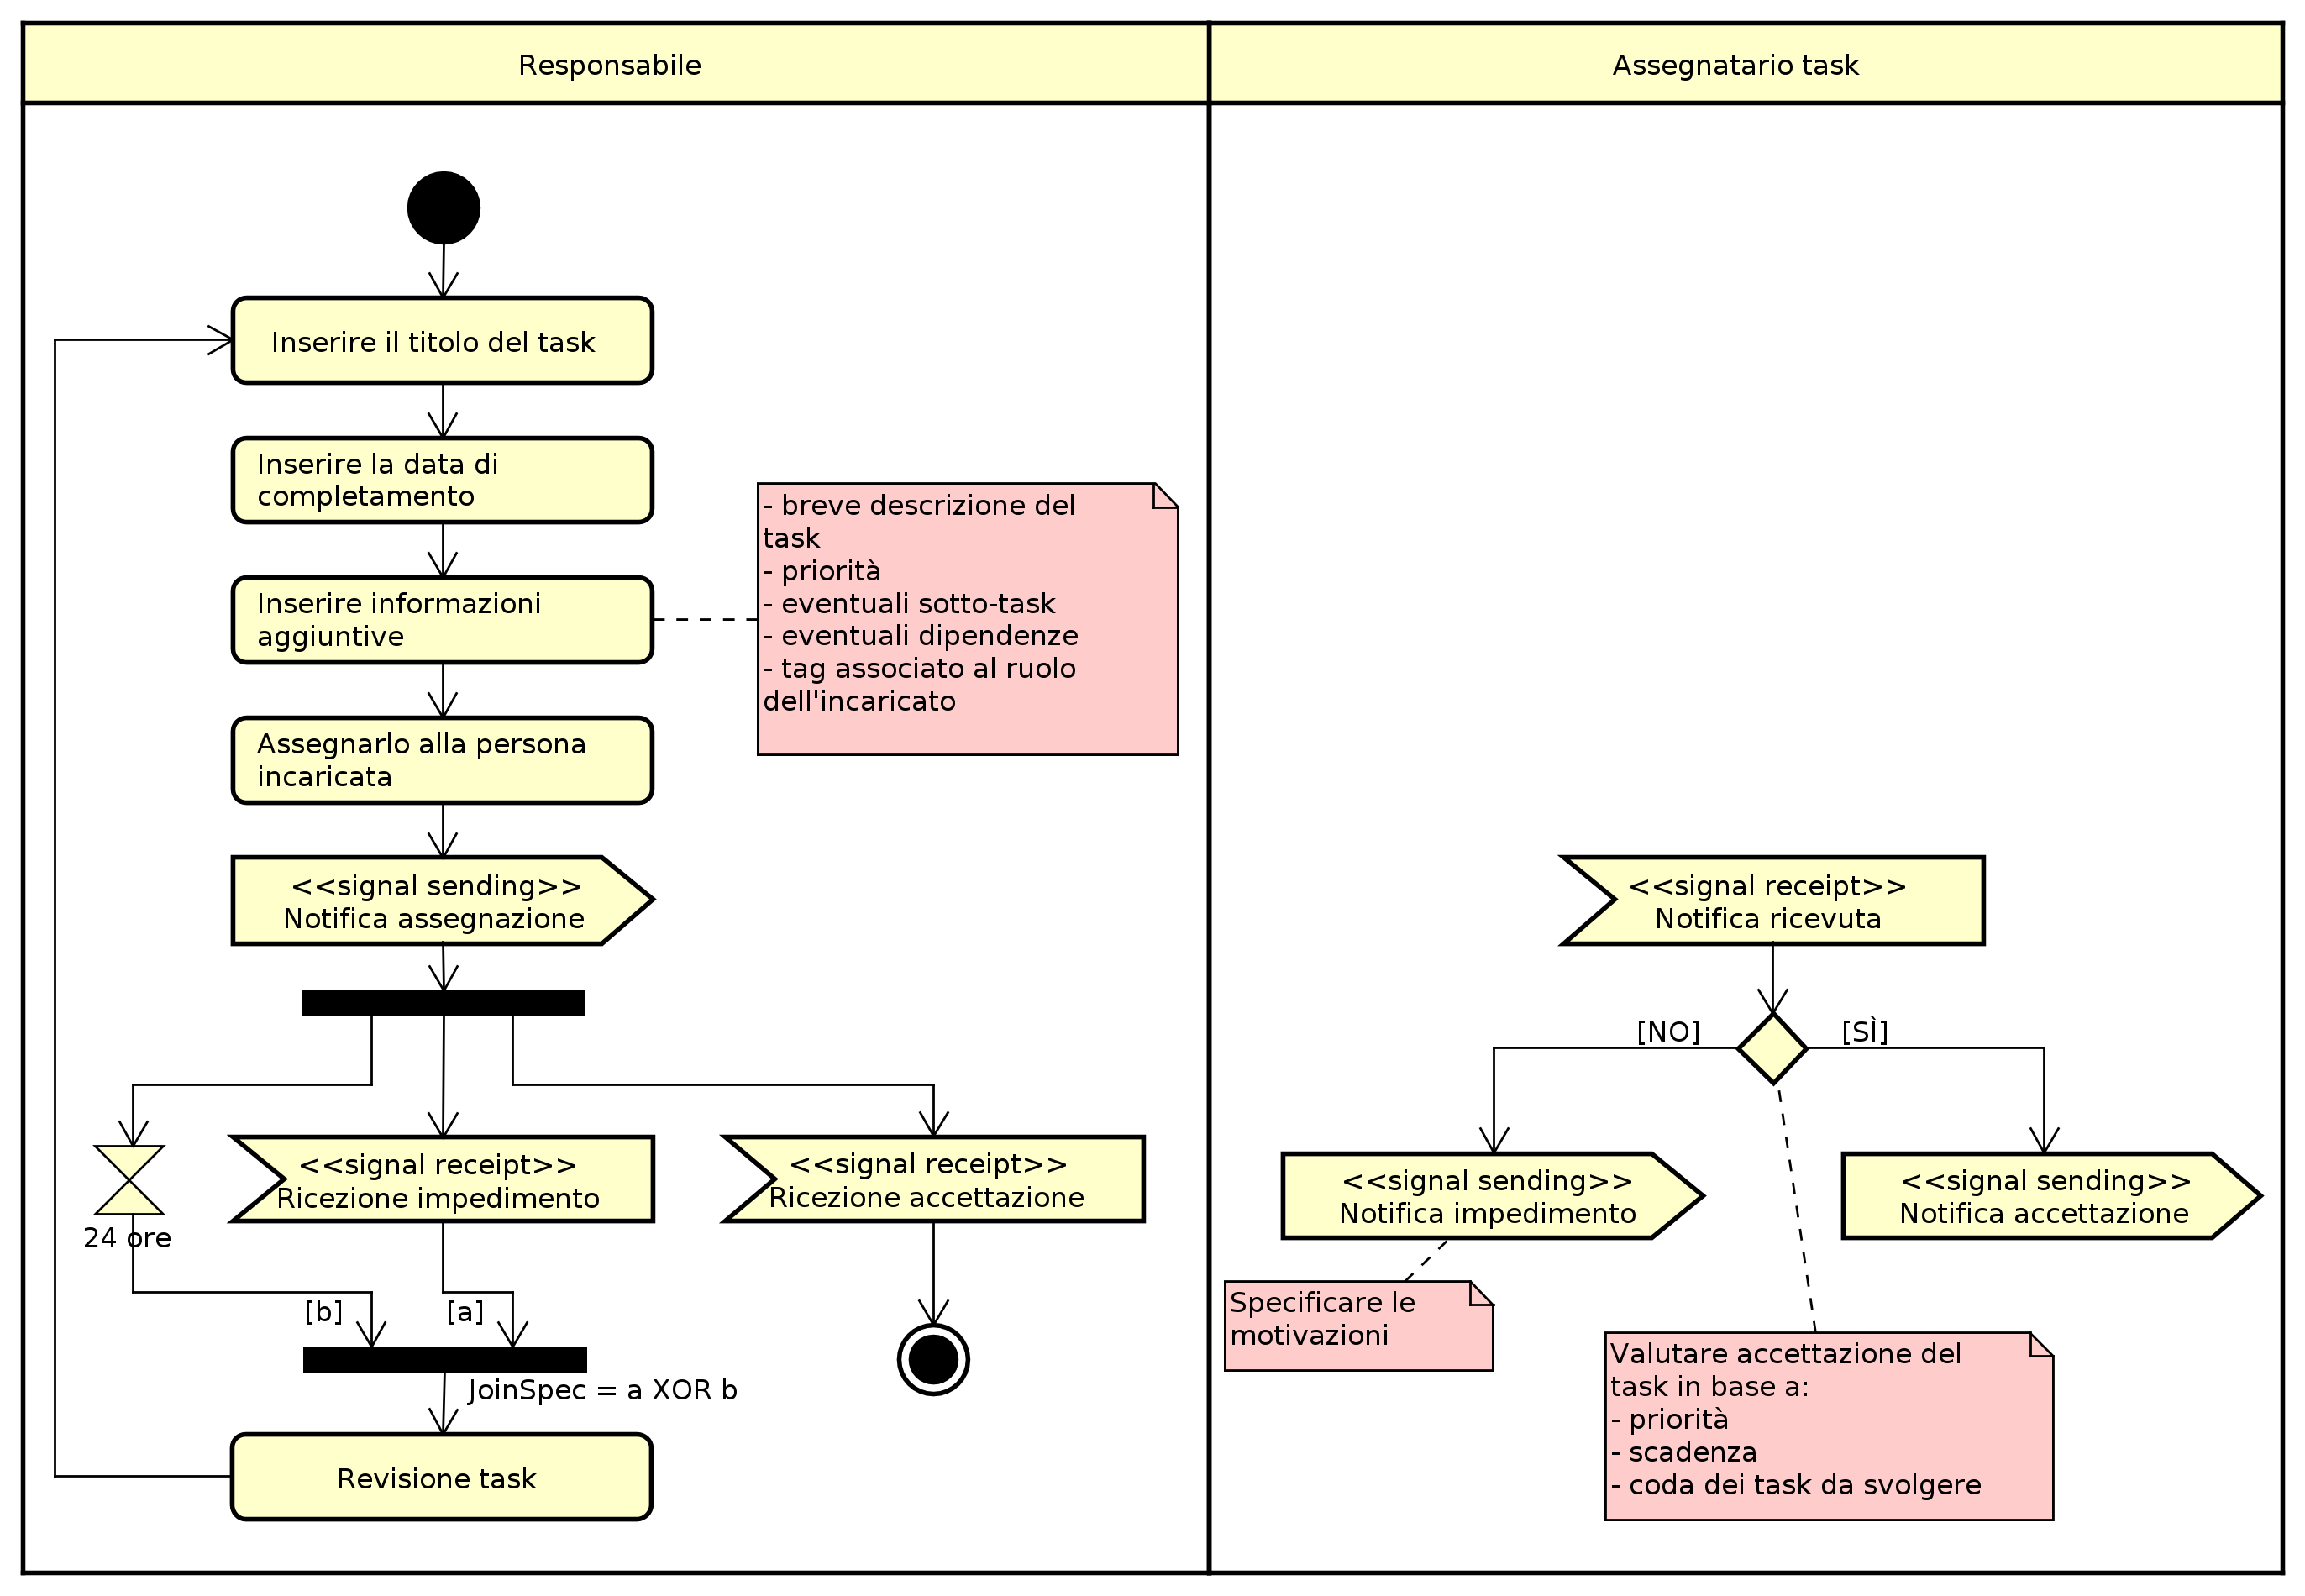
\includegraphics[width=\textwidth]{img/proc_ass_ticket.png}
	    		        \caption{Procedura assegnazione ticket. Riferita nella sezione \ref{sec:creazioneticket}}
	                    \label{fig:procassticket}
	    	        \end{figure}\mbox{}\\
	            \subparagraph{Modifica di un ticket}\label{sec:modificaticket}
	                La modifica di un ticket deve essere svolta rispettando il seguente ordine:
	                \begin{enumerate}
	                	\item ricerca del ticket da modificare;
	                	\item modifica di uno o più campi;
	                	\item verifica inserimento dei campi dati: titolo, assegnatario, descrizione e data di completamento;
	                	\item salvare le modifiche apportate.
	                \end{enumerate}
	                Vedi figura \ref{fig:procmodticket}.
	                    \begin{figure}[h!]
	                        \centering
	        	        	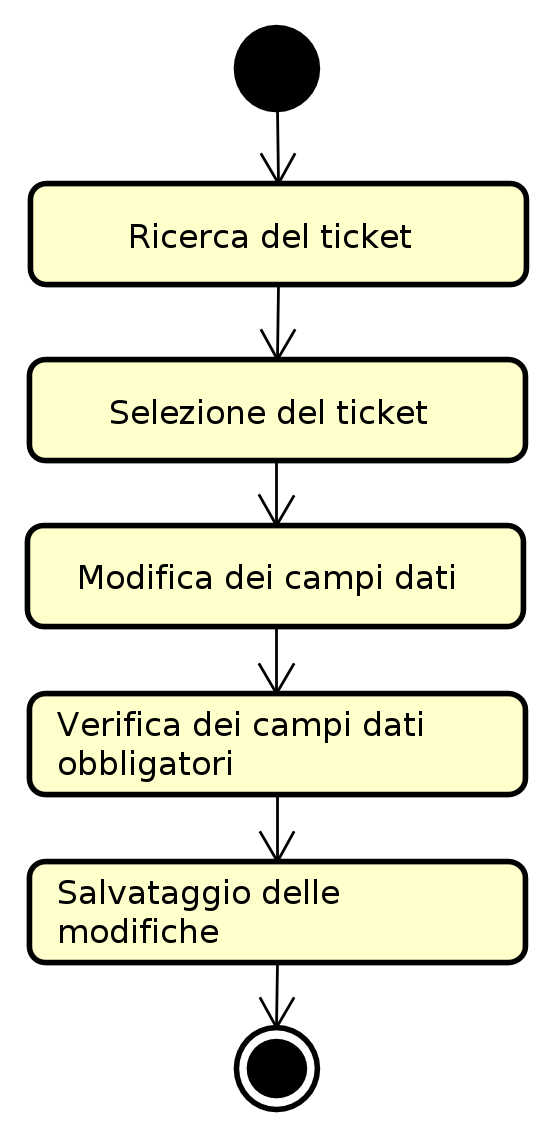
\includegraphics[width=0.3\textwidth]{img/proc_mod_ticket}
	                        \caption{Procedura modifica ticket. Riferita nella sezione \ref{sec:modificaticket}}
	                        \label{fig:procmodticket}
	        	        \end{figure}\mbox{}\\
	            \subparagraph{Chiusura di un ticket}\label{sec:chiusuraticket}
	            La chiusura di un ticket da parte dell'incaricato deve essere svolta rispettando la seguente procedura:
	            \begin{enumerate}
	            	\item ricerca del ticket da chiudere;
	            	\item aprire le proprietà del ticket e cliccare su \hicode{"Log time"};
	            	\item se il ticket è relativo ad un task di modifica di un documento:
	            	\begin{enumerate}
	            		\item eseguire un commit con solo l'aggiornamento del registro delle modifiche del documento;
	            		\item copiare il codice del commit ed inserirlo nella descrizione del task;
	            		\item eseguire il push delle modifiche.
	            	\end{enumerate}
	            	\item inserire il tempo speso per completare il task;
	            	\item selezionare \hicode{"Billable"} se il tempo speso è rendicontabile;
	            	\item selezionare \hicode{"Task is now complete"};
	            	\item cliccare su \hicode{"Log this time"}.
	            \end{enumerate}
	            Vedi figura \ref{fig:procChiusuraTicket}.\\\\
	            Una procedura automatica implementata nella chat Slack controllerà che il codice del commit inserito nel task sia presente nei messaggi inviati da GitHub, se così non fosse provvederà ad inviare un avviso al \responsabilediprogetto.
	        %
	        \begin{figure}[h!]
	        	\centering
	        	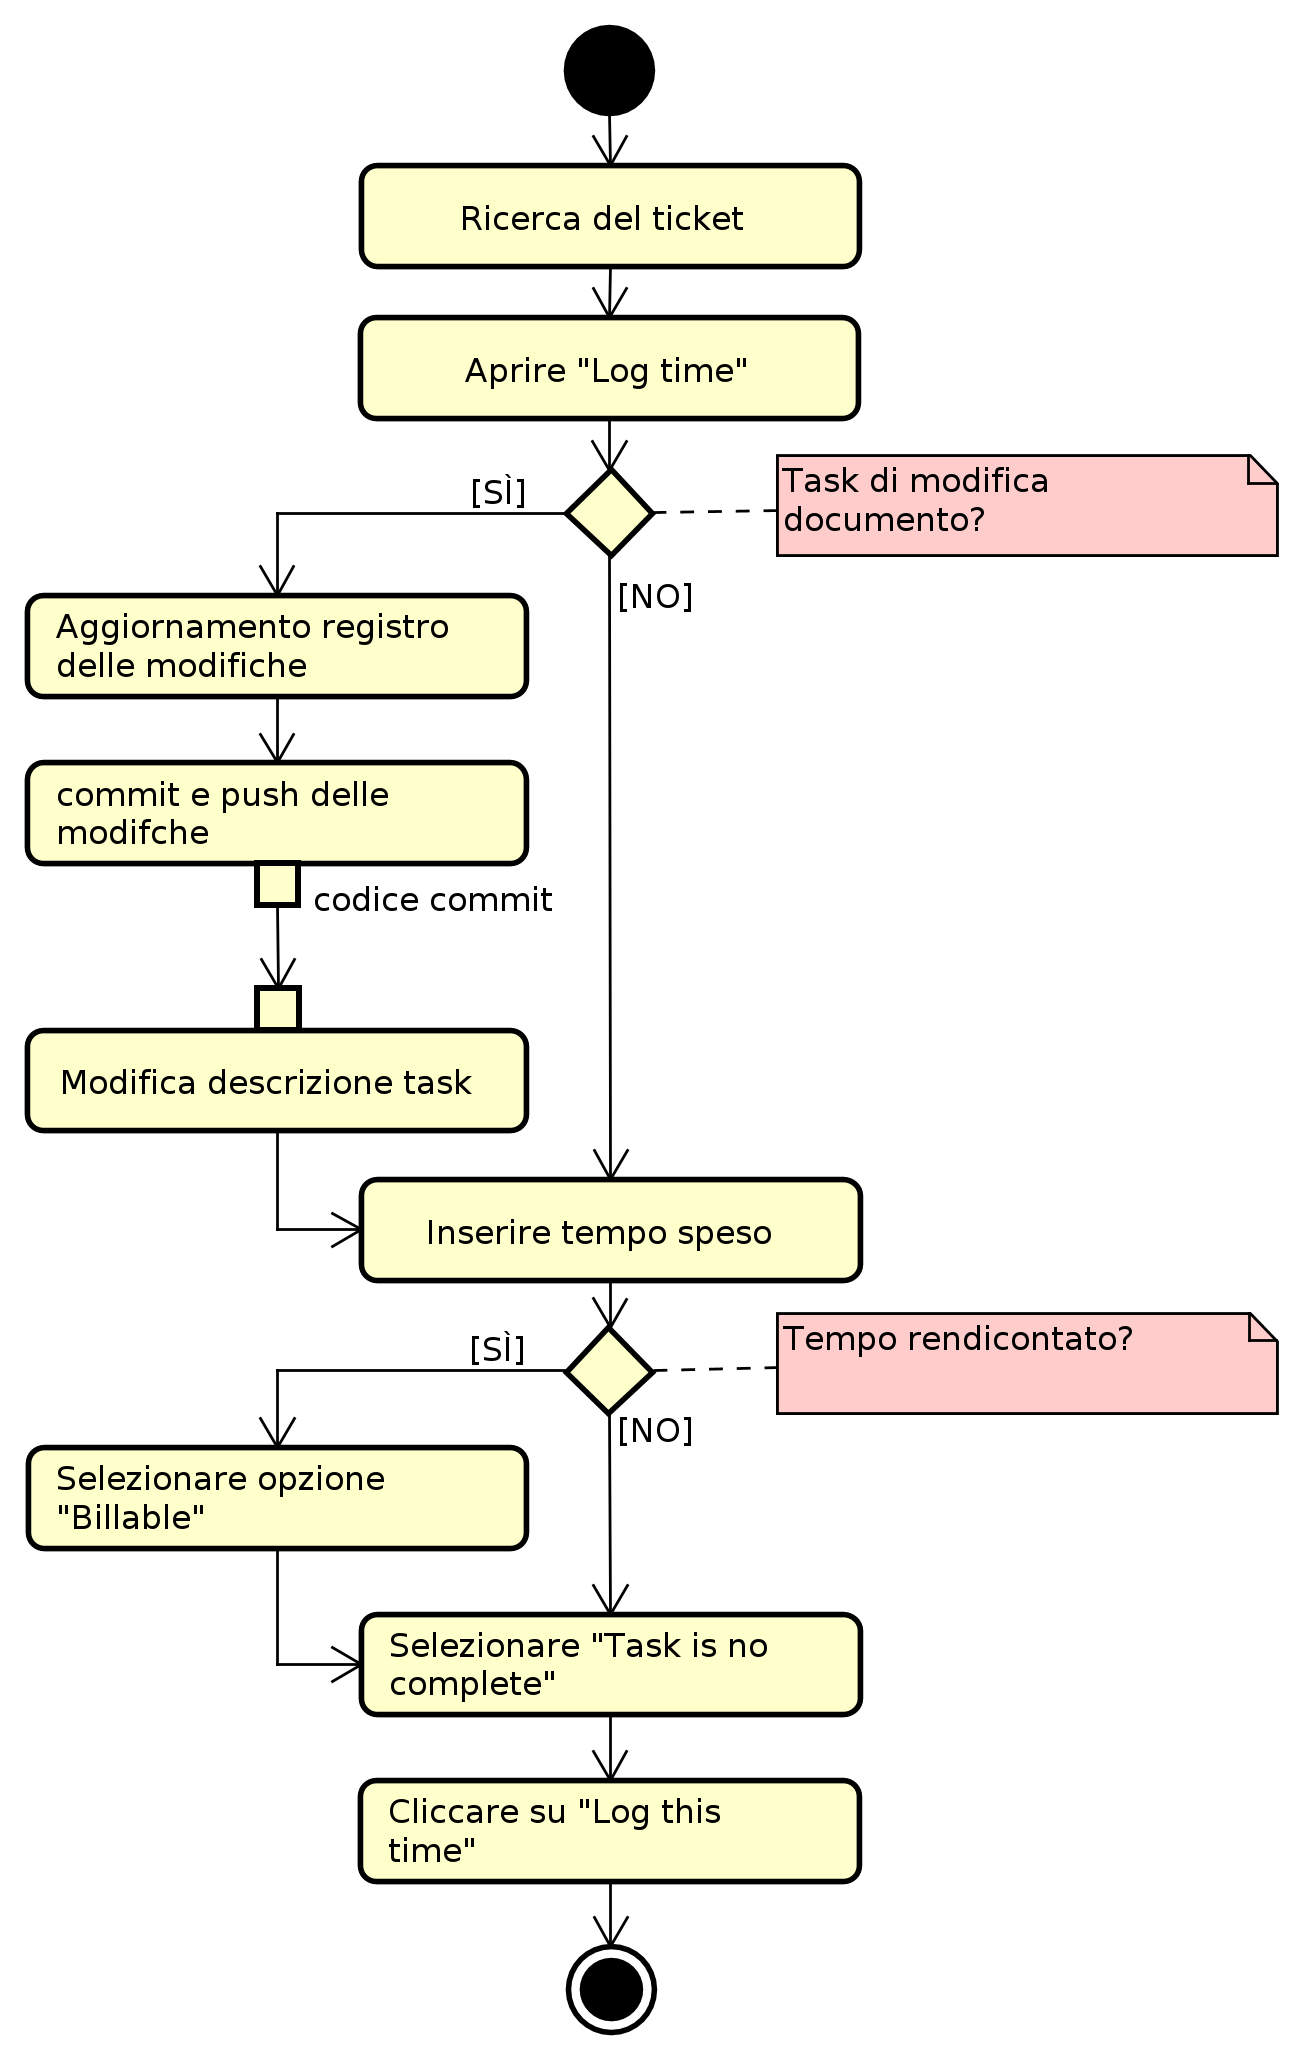
\includegraphics[width=0.6\textwidth]{img/proc_chiusura_ticket.png}
	        	\caption{Procedura chiusura ticket. Riferita nella sezione \ref{sec:chiusuraticket}}
	        	\label{fig:procChiusuraTicket}
	        \end{figure}\mbox{}\\
	        %
            \paragraph{Gestione delle milestone}
            Accedere allo spazio Teamwork del gruppo, posizionandosi nella sezione \textit{"Milestones"} oppure tramite il seguente link: \url{https://swe2016.teamwork.com/#/projects/140646/milestones/upcoming}. Premere su \textit{"Add \glo{Milestone}{Milestone}"} per la creazione o sul nome di una milestone esistente per la modifica.
            \subparagraph{Creazione milestone}\label{sec:creazionemilestone}
                La creazione di una milestone deve essere svolta rispettando il seguente ordine:
    			\begin{enumerate}
    				\item inserimento titolo milestone;
    				\item inserimento data;
    				\item assegnazione persone coinvolte;
    				\item assegnazione reminders;
    				\item inserimento descrizione;
    				\item salvataggio milestone.
    			\end{enumerate}
                Vedi figura \ref{fig:procinsmilestone}.
    			\begin{figure}[h!]
                    \centering
    				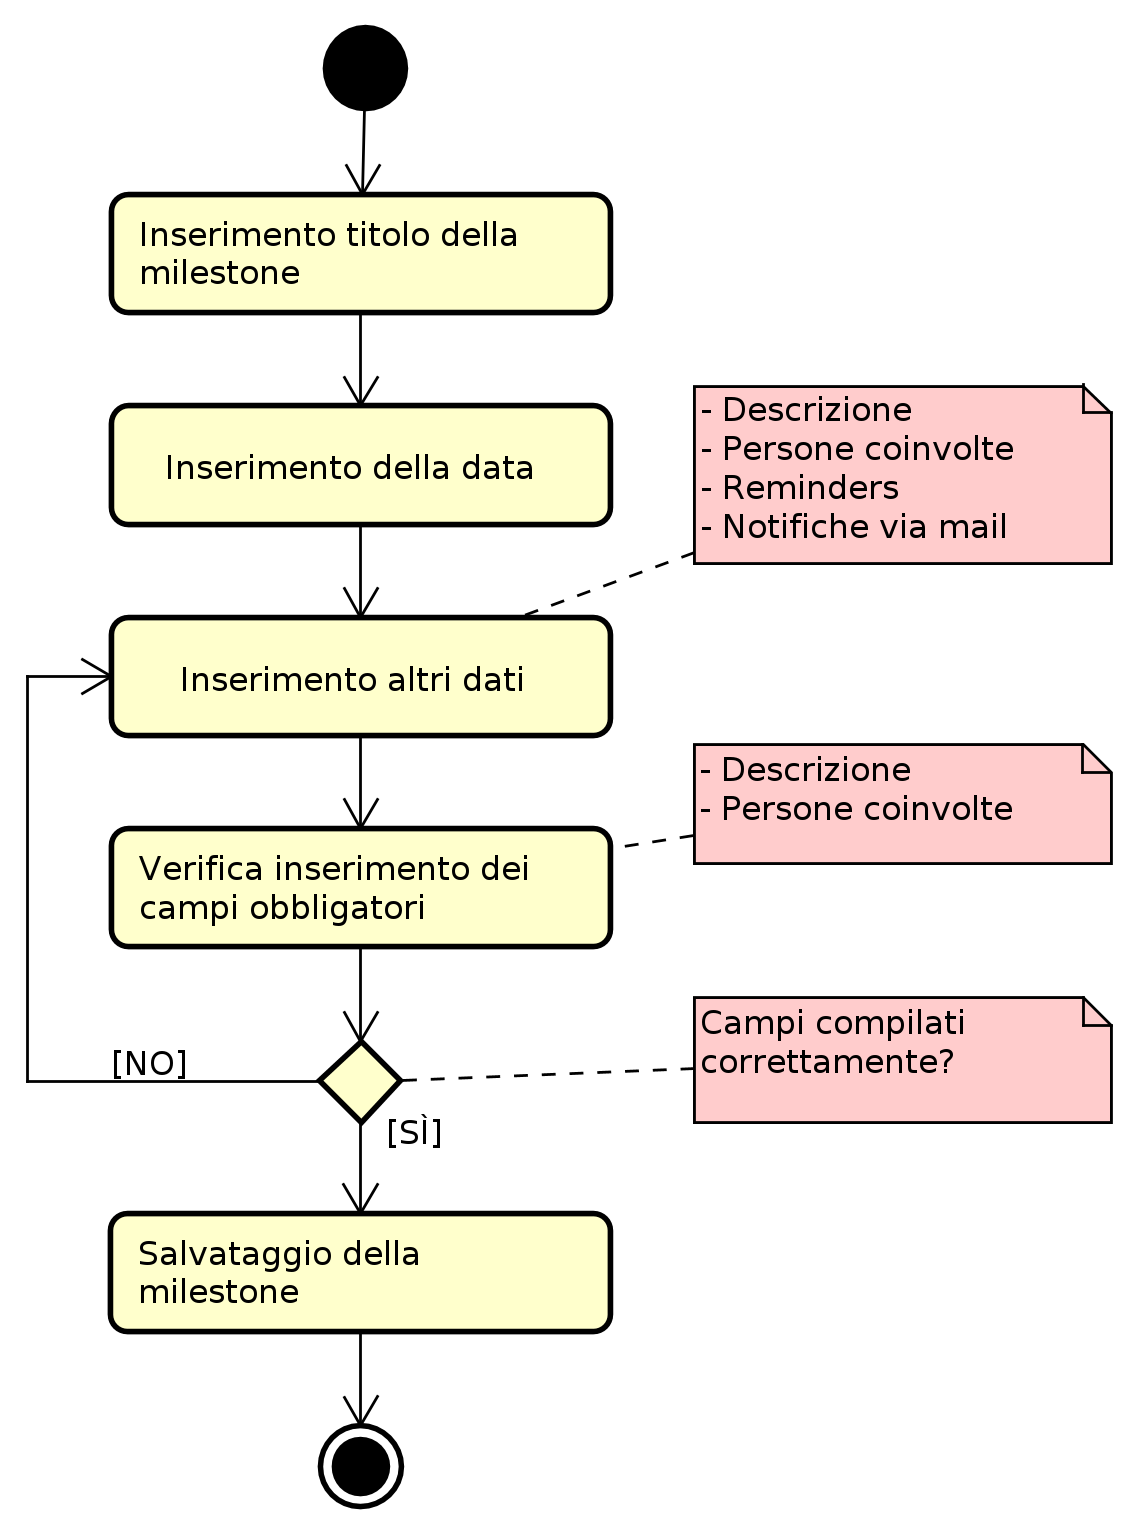
\includegraphics[width=0.5\textwidth]{img/proc_ins_milestone}
    				\caption{Procedura inserimento milestone. Riferita nella sezione \ref{sec:creazionemilestone}}
                    \label{fig:procinsmilestone}
    			\end{figure}\mbox{}\\
            \subparagraph{Modifica milestone}\label{sec:modificamilestone}
			La modifica di una milestone deve essere svolta rispettando il seguente ordine:
    			\begin{itemize}
    				\item selezione milestone;
    				\item modifica di uno o più campi dati;
    				\item verifica inserimento dei campi dati: titolo, data, descrizione e assegnatari;
    				\item salvataggio milestone.
    			\end{itemize}
                Vedi figura \ref{fig:procmodmilestone}.
        		\begin{figure}[h!]
                    \centering
        			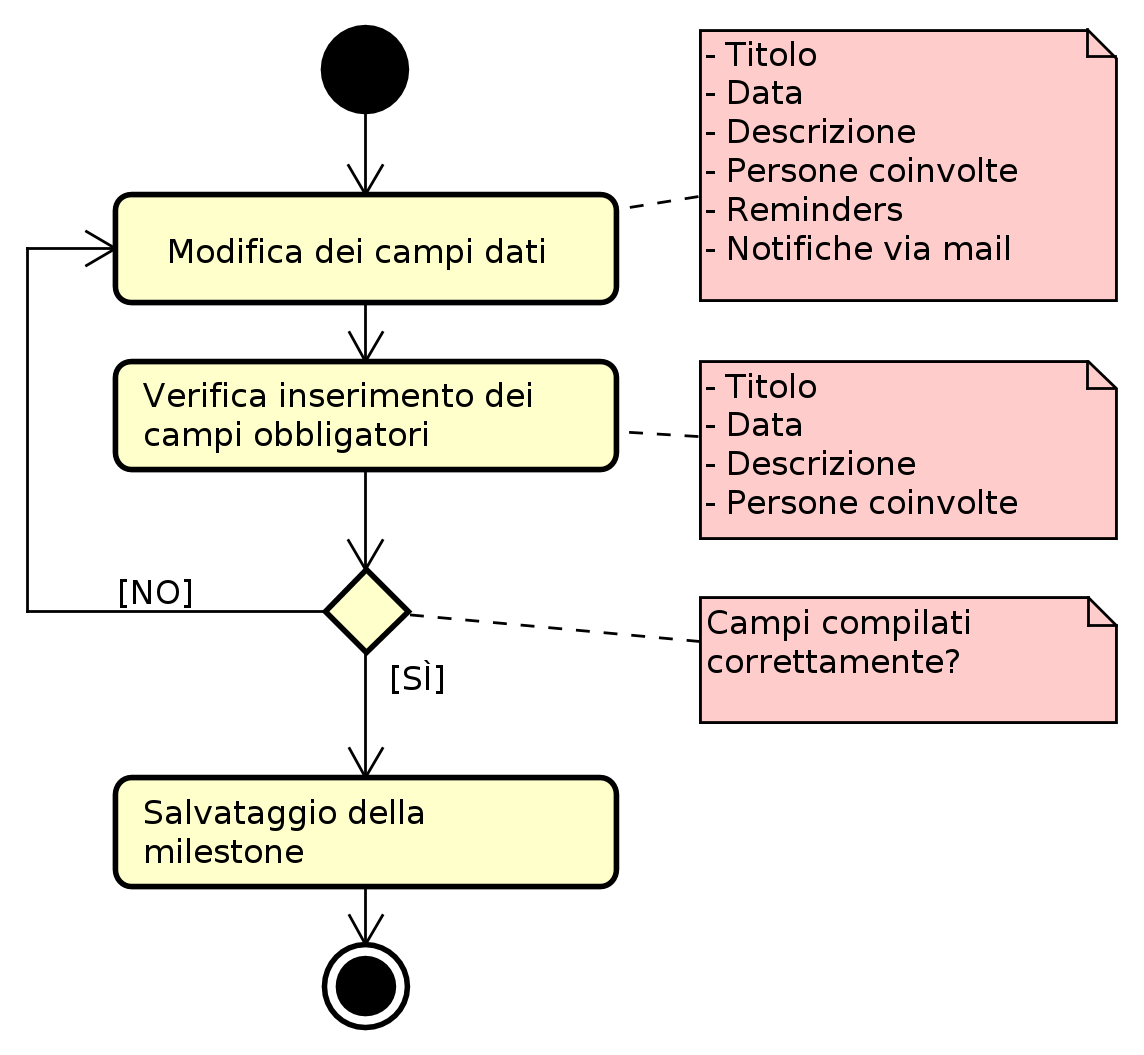
\includegraphics[width=0.5\textwidth]{img/proc_mod_milestone}
        			\caption{Procedura modifica milestone. Riferita nella sezione \ref{sec:modificamilestone}}
                    \label{fig:procmodmilestone}
        		\end{figure}\mbox{}\\
        %
       	\paragraph{Creazione nuovo canale Slack}\label{sec:CreaCanale}
		La creazione di un nuovo canale Slack può essere fatta solo da parte del \responsabile{} e deve rispettare il seguente ordine:
		\begin{enumerate}
			\item effettuare il login su Slack nel sito o nell'applicazione, con l'utente \textit{zephyrus.swe};
			\item cliccare nel menù di sinistra la voce \hicode{CHANNELS};
			\item cliccare il pulsante \hicode{New Channel};
			\item scegliere se rendere il canale pubblico o privato;
			\item scegliere il nome del canale;
			\item compilare l'eventuale descrizione riguardo la tematica del canale;
			\item inserire i nomi delle persone che si desidera invitare;
			\item cliccare sul bottone \hicode{Create Channel}.
		\end{enumerate}
		Vedi figura \ref{fig:ProCreaCanale}.
		\begin{figure}[h!]
			\centering
			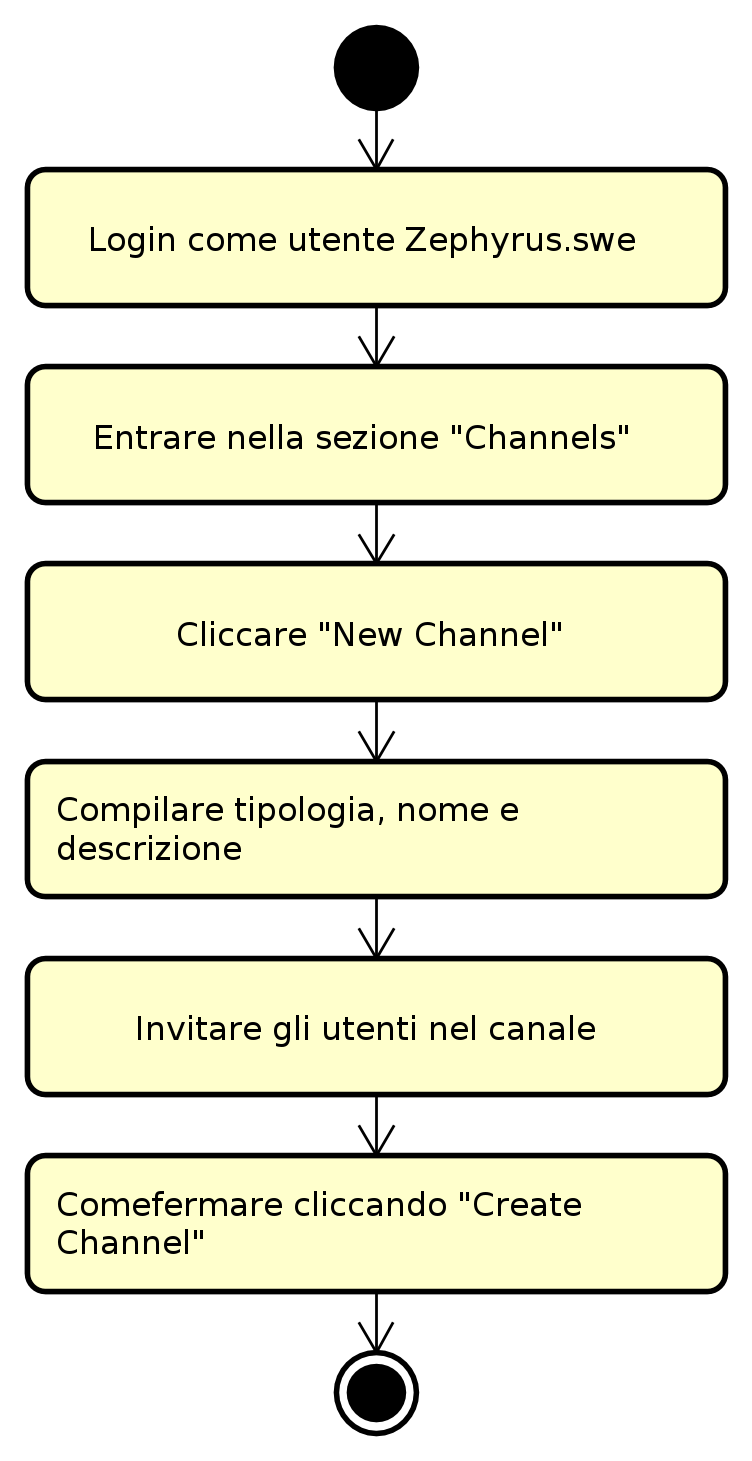
\includegraphics[width=0.3\textwidth]{img/CreazioneCanaleSlack}
			\caption{Procedura di creazione di un canale Slack. Riferita nella sezione \ref{sec:CreaCanale}}
			\label{fig:ProCreaCanale}
		\end{figure}\mbox{}\\
		%
		\paragraph{Modifica impostazioni canale Slack}\label{sec:ModCanale}
		In un canale Slack si possono modificare varie impostazioni, tra cui: 
		\begin{itemize}
			\item invitare o rimuovere membri;
			\item preferenze di notifica;
			\item integrare app esterne;
			\item silenziare il canale;
			\item uscire dal canale.
		\end{itemize}
		Tranne la prima, tutte le altre sono a discrezione dell'utente. Di seguito si presenta la procedura eseguibile solo dal \responsabile{} per aggiungere un membro al canale. 
		\begin{enumerate}
			\item effettuare il login su Slack nel sito o nell'applicazione, con l'utente \hicode{zephyrus.swe};
			\item cliccare nel canale che si desidera apportare modifiche;
			\item cliccare il pulsante con l'icona a forma di ingranaggio e successivamente \hicode{Invite team Members};
			\item inserire il nickname della persona che si vuole aggiungere;
			\item cliccare sul bottone \hicode{Invite}.
		\end{enumerate}
		N.B. Per poter visualizzare il nome della persona da aggiungere è necessario che quest'ultima faccia già parte del Team su Slack, in caso contrario bisogna invitarla tramite indirizzo mail.
		Vedi figura \ref{fig:ProModChannel}.
		\begin{figure}[h!]
			\centering
			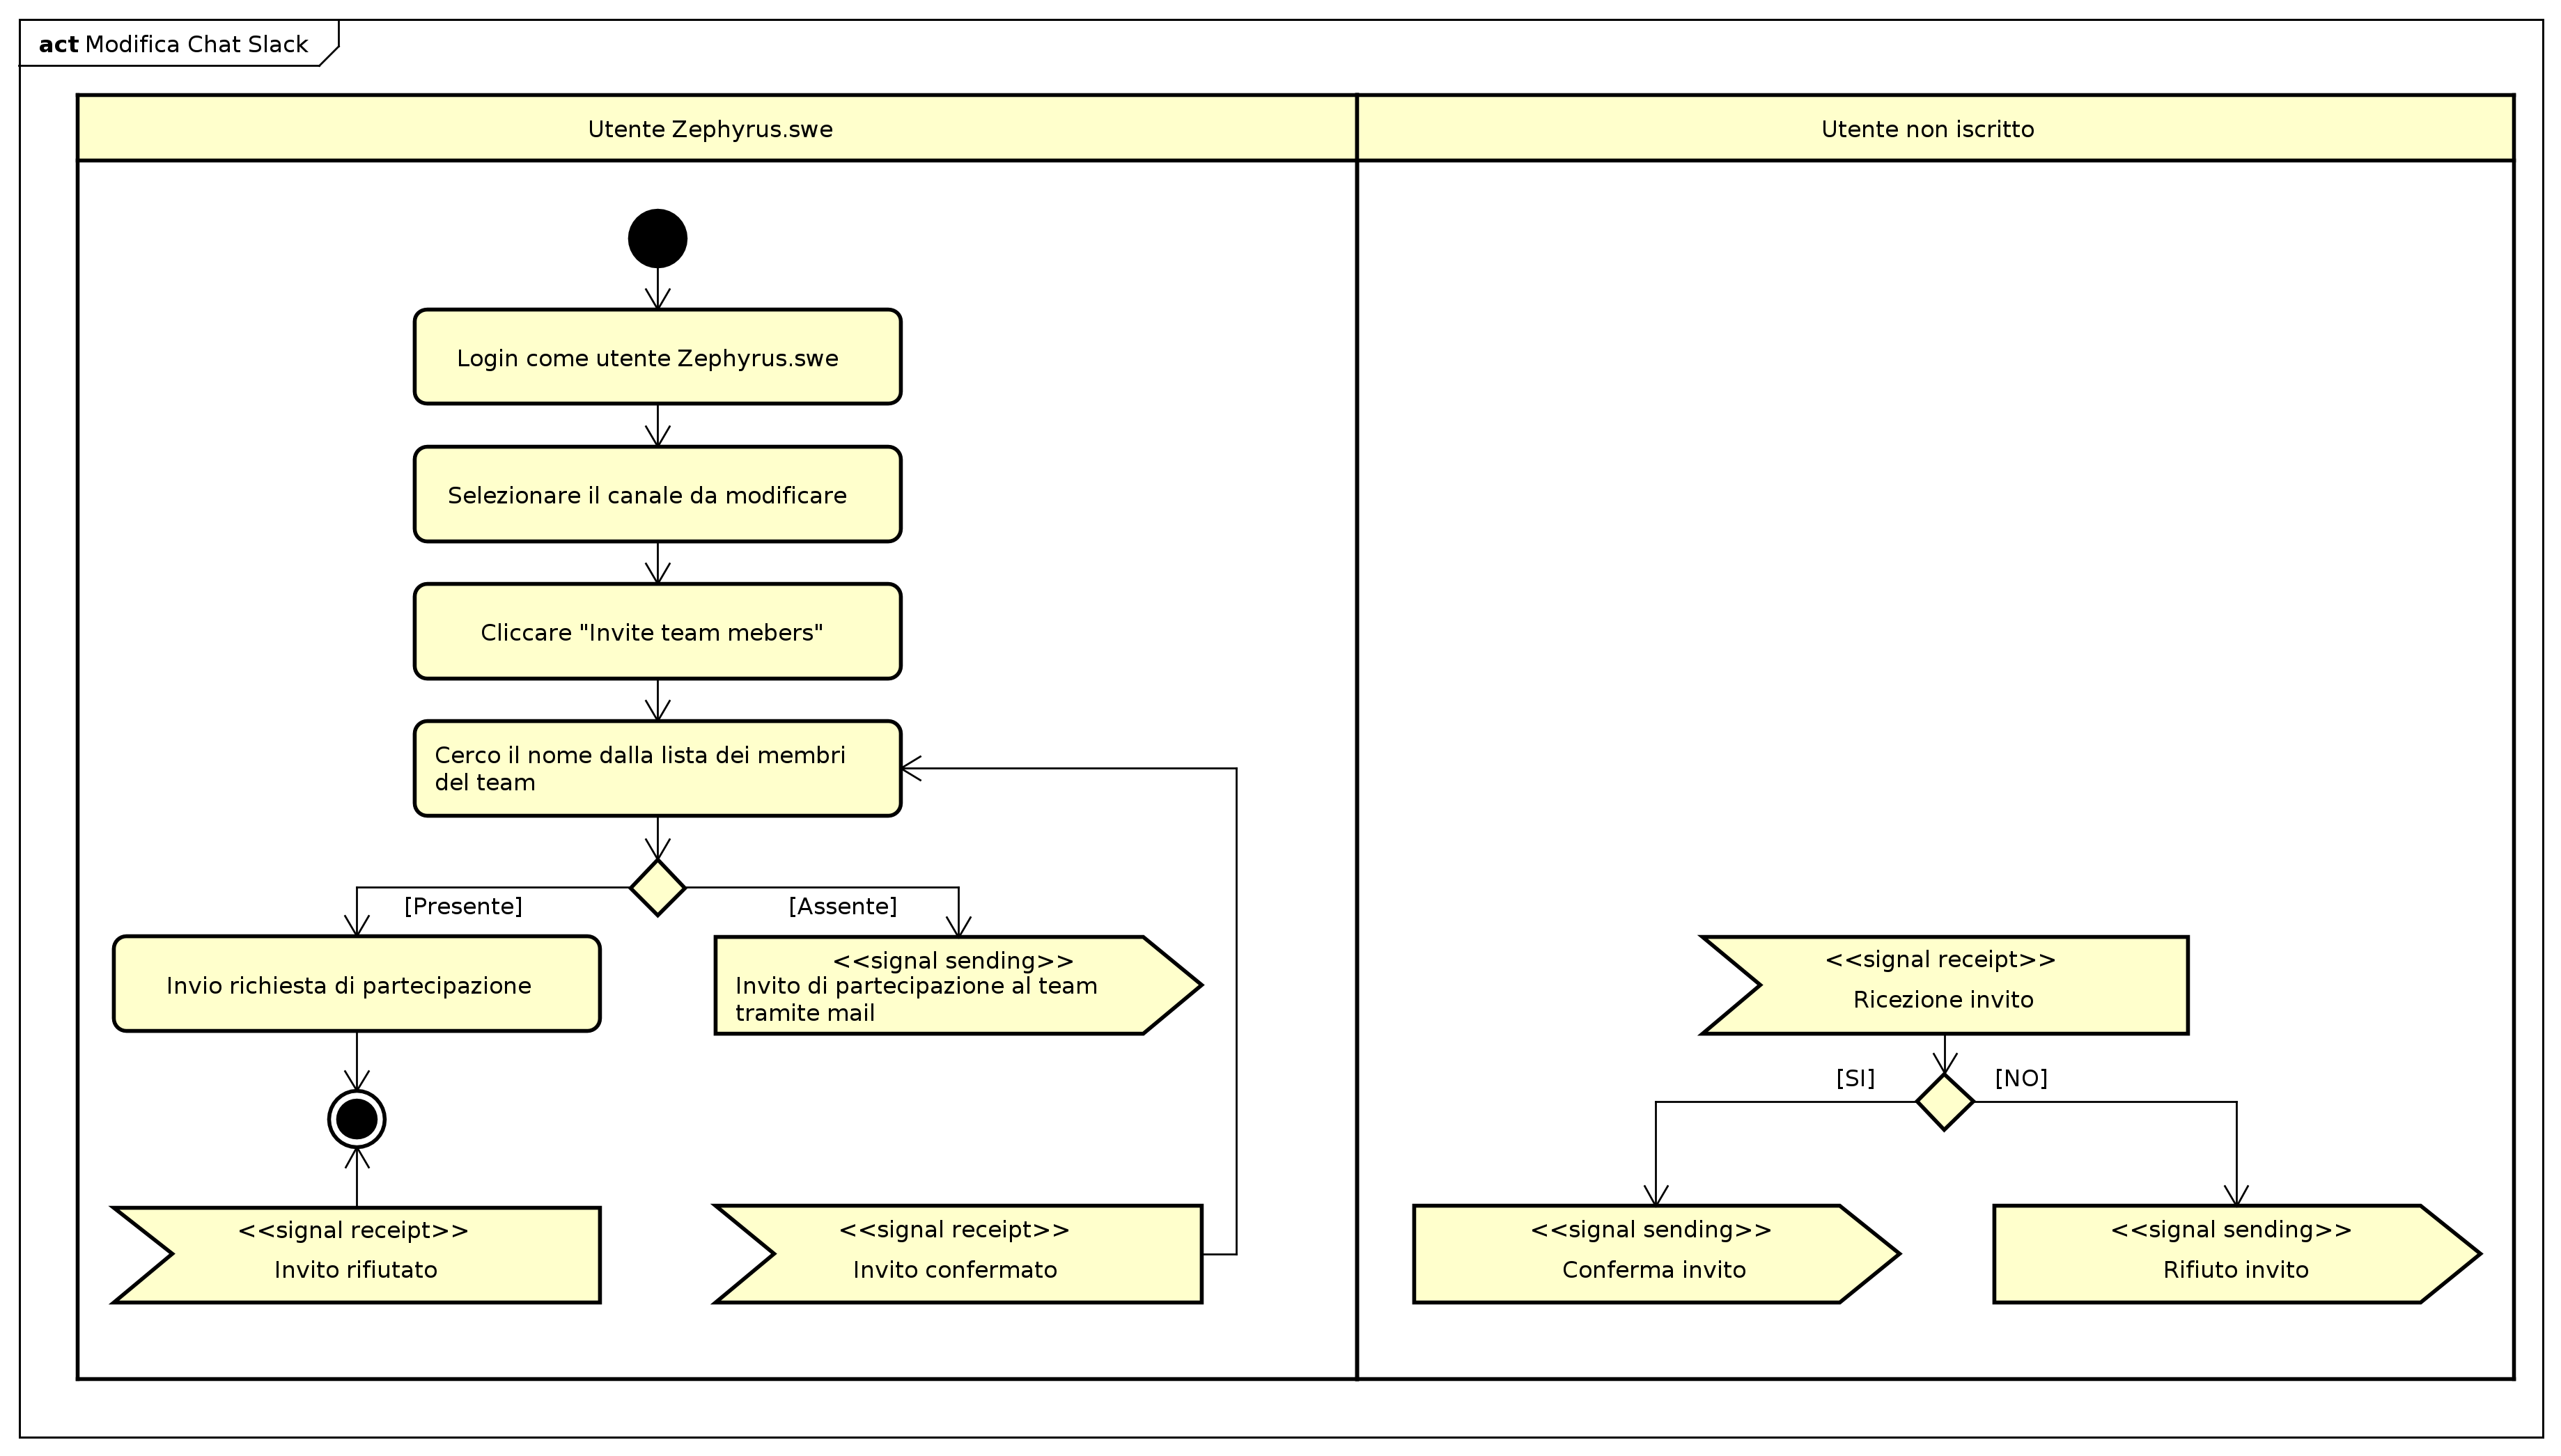
\includegraphics[width=\textwidth]{img/ProModChannel}
			\caption{Procedura di creazione di un canale Slack. Riferita nella sezione \ref{sec:ModCanale}}
			\label{fig:ProModChannel}
		\end{figure}\mbox{}\\	
	
        
    \subsection{Gestione delle infrastrutture}
        \subsubsection{Scopo}
        Lo scopo del processo di gestione delle infrastrutture è di stabilire e mantenere le infrastrutture e gli strumenti necessari allo svolgimento dei processi durante lo svolgimento del progetto. La corretta implementazione del processo deve:
        \begin{itemize}
            \item fornire un ambiente di lavoro idoneo;
            \item garantire il funzionamento di tutte le infrastrutture necessarie;
            \item indicare il corretto utilizzo delle infrastrutture.
        \end{itemize}

		\subsubsection{Ambiente di sviluppo}
		L'\amministratore{} ha il compito di decidere l'ambiente ottimale per lo sviluppo e il test dell'applicazione. Se necessario è possibile coinvolgere il proponente nella decisione, in questo caso sarà compito del \responsabilediprogetto{} organizzare le riunioni o i contatti necessari.
		Una volta deciso l'ambiente di sviluppo l'\amministratore{} dovrà indicare a tutti i membri del gruppo le procedure necessarie per il suo corretto utilizzo, eventuali modifiche o aggiornamenti dovranno essere segnalati tempestivamente tramite gli appositi canali di comunicazione.

        \subsubsection{Aggiornamento applicazioni}
        L'\amministratore{} ha il compito di informare tutti i membri del gruppo di eventuali aggiornamenti disponibili per applicazioni in uso e se una loro installazione potrebbe generare incompatibilità con altri strumenti.
        Inoltre deve mantenere aggiornato, situato nello spazio Google Drive, il documento condiviso:
        \begin{center}
        	\texttt{Strumenti utilizzati}
        \end{center}
        contenente le versioni degli strumenti installati per ogni membro del gruppo.
        
        \subsubsection{Gestione account e password}
        L'\amministratore{} ha il compito di mantenere aggiornato il documento contenente le informazioni riguardanti gli account degli strumenti e dei siti in uso per lo svolgimento del progetto, comunicando eventualmente le variazioni ai membri del gruppo interessati. Inoltre deve monitorare l'utilizzo degli spazi per la condivisione dei file per assicurarsi che vengano utilizzati unicamente per gli scopi del progetto e per garantire che tutti i membri del gruppo possano accedervi senza limitazioni.
        
		\subsubsection{Gestione comunicazioni}
		L'\amministratore{} ha il compito di controllare e gestire i canali presenti nella chat Slack per mantenere un livello di conversazione accettabile e costruttivo fra tutti i membri del gruppo e per garantire che la chat non venga utilizzata impropriamente.
		Nello specifico l'\amministratore{} dovrà:
		\begin{itemize}
			\item assicurarsi che il linguaggio utilizzato sia rispettoso di tutti i membri del gruppo e consono all'ambiete di lavoro;
			\item assicurarsi che ogni canale venga utilizzato unicamente allo scopo preposto;
			\item se necessario, creare nuovi canali e invitarvi i membri del gruppo che li dovranno utilizzare;
			\item archiviare canali non più utilizzati se ritenuto opportuno;
			\item eliminare messaggi ritenuti inopportuni o non in linea con le indicazioni di cui sopra;
			\item gestire eventuali estensioni di Slack;
			\item farsi carico di eventuali lamentele o segnalazioni da parte dei membri del gruppo e riportarle al \responsabilediprogetto{} se necessario.
		\end{itemize}
	%
	\subsubsection{Strumenti}
	\paragraph{Integrazioni Slack} \label{sec:intSlack}
	L'\amministratore{} ha il compito di controllare e gestire le integrazioni della chat Slack:
	\begin{itemize}
		\item \textbf{Teamwork:} il canale \hicode{\#task} dovrà contenere tutti i messaggi provenienti da Teamwork e relativi alla creazione, modifica e chiusura dei ticket;
		\item \textbf{GitHub:} il canale \hicode{\#dev} dovrà contenere tutti i messaggi provenienti dai commit eseguiti sui repository git utilizzati;
		\item \textbf{Condivisione:} il canale \hicode{\#share} dovrà contenere tutti i messaggi provenienti dalle modifiche eseguite su Dropbox o GoogleDrive.
	\end{itemize}
	%
	\paragraph{Node.js} \label{nodejs}
	\glo{Node.js}{Node.js} è una piattaforma event-driven per il motore \glo{JavaScript}{JavaScript} V8, disponibile sulle principali piattaforme, anche se maggiormente performante su sistemi operativi UNIX-like.
	L'indirizzo per il download e la documentazione:
	\begin{center}
		\url{https://nodejs.org/en/download/}
	\end{center}
	%
	\paragraph{npm}
	npm (node package manager) è il gestore di pacchetti di default utilizzato da Node.js. Questo strumento consente  l'installazione e la gestione di moduli esterni che forniscono funzionalità aggiuntive al sistema node di base, risolvendo varie dipendenze.
	Le principali motivazioni che hanno portato il gruppo alla scelta di questo strumento sono:
	\begin{itemize}
		\item larga diffusione;
		\item più di 400.000 pacchetti installabili;
		\item ampia documentazione.
	\end{itemize}
	Indirizzo per il download e la documentazione:
	\begin{center}
		\url{https://www.npmjs.com}
	\end{center}
	\paragraph{Sistemi operativi}
	I membri del gruppo operano sui seguenti sistemi operativi:
	\begin{itemize}
		\item \glo{Linux}{Linux} distribuzioni: Debian v8.0, Ubuntu v16.04 e superiori;
		\item \glo{Windows}{Windows} versione: 10;
		\item \glo{MacOS}{MacOS} versione: 10.12.
	\end{itemize}
	%
	\paragraph{VirtualBox}
	% 1)descrizione veloce dell'app
	VirtualBox è un'applicazione opensource e gratuita sviluppata da Oracle per l'esecuzione di macchine virtuali,
	% 2)cosa ci permette di fare
	permette quindi di eseguire ed utilizzare all'interno di qualsiasi computer un sistema virtualizzato con caratteristiche diverse dal sistema che lo ospita.
	% 3) perche l'abbiamo scelta
	L'applicazione è stata scelta di comune accordo con il proponente, che fornirà l'immagine di una macchina virtuale con le caratteristiche necessarie per poter essere utilizzata come ambiente di sviluppo e test.\\
	% 4) indirizzo dove collegarsi
	VirtualBox è disponible per tutti i principali sistemi operativi e la sua installazione non prevede procedure particolari. La versione utilizzata è quella stabile, oltre all'applicazione è necessario installare anche l'\textit{Extension Pack}. Tutte le informazioni necessarie al download e all'installazione possono essere trovate al seguente indirizzo:\\
	\begin{center}
		\url{https://www.virtualbox.org/wiki/Downloads}
	\end{center}
	%
	\paragraph{FileZilla Client}
	% 1)descrizione veloce dell'app
	FileZilla Client è un software opensource cross-platfom che permette il trasferimento di file in rete attraverso il protocollo FTP.
	
	Il programma è disponibile per i sistemi operativi Linux, Microsoft Windows, e macOS. Tra i vari protocolli supportati, oltre all'FTP c'è l'SFTP, e l'FTP su SSL/TLS.
	% 3) perche l'abbiamo scelta
	Le principali motivazioni che hanno portato il gruppo alla scelta di questo strumento sono:
	\begin{itemize}
		\item applicazione semplice e leggera;
		\item già conosciuta da molti membri del gruppo.
	\end{itemize}
	Indirizzo per il download e la documentazione:
	\begin{center}
		\url{https://filezilla-project.org/download.php?type=client}
	\end{center}
	%	
	\subsubsection{Procedure}
	\paragraph{Backup}
	Con cadenza mensile l'\amministratore{} deve eseguire un backup su dispositivo esterno dei seguenti dati:
	\begin{itemize}
		\item \glo{Database}{database} \glo{Trender}{Trender};
		\item repository Documenti;
		\item repository Codice;
		\item cartella Dropbox.
	\end{itemize}
	%
	\paragraph{Configurazione VirtualBox}
	La macchina virtuale fornita da \riskapp{} deve essere configurata per poter consentire un agevole ambiente di sviluppo e test per il progetto.
	
	Inizialmente si configura la VirtualBox precedentemente installata seguendo i seguenti passi:
	\begin{enumerate}
		\item aprire VirtualBox;
		\item entrare nel menù \hicode{File -> Preferences -> Network -> NAT Networks};
		\item cliccare sul bottone \hicode{"+" (Add)};
		\item cliccare sul bottone \hicode{Edit};
		\item cliccare su \hicode{"Port Forwarding"};
		\item selezionare \hicode{IPv4};
		\item cliccare sul bottone \hicode{"+" (Add)};
		\item editare i campi in modo da avere le seguenti due regole:  \\
		\begin{table}[H]
			\centering
			\begin{tabular}{|llllll|}
				\hline
				Name & Protocol & Host IP & Host Port & Guest IP & Guest Port \\ \hline
				Rule 1 & TCP & 127.0.0.1 & 10080 & 10.0.2.15 & 80 \\ \hline
				Rule 2 & TCP & 127.0.0.1 & 10022 & 10.0.2.15 & 22 \\ \hline
			\end{tabular}
		\end{table}
		\item chiudere le finestra cliccando su \hicode{Ok}.
	\end{enumerate}
	In questo modo si può testare il sito dal browser del proprio PC invece che da quello della macchina virtuale, aprendo il browser e digitando l'URL \url{http://localhost:10080}.
	%
	Successivamente si procede con la configurazione della macchina virtuale precedentemente installata come descritto nella sezione \ref{installazioneMacchinaVirtuale} rispettando i seguenti passi:
	\begin{enumerate}
		\item aprire Virtualbox;
		\item cliccare con il tasto destro sulla macchina virtuale "Zephyrus" \hicode{Settings -> Network};
		\item impostare il campo "Connect to:" a \hicode{Nat Network};
		\item impostare il campo "Name" a \hicode{NatNetwork};
		\item chiudere le finestre cliccando sul bottone \hicode{Ok};
		\item avviare la macchina virtuale premendo sul bottone \hicode{Start}.
	\end{enumerate}
	%
	\paragraph{Installazione macchina virtuale} \label{installazioneMacchinaVirtuale}
	\begin{enumerate}
		\item Scaricare il file con l'immagine dal seguente link:
		\begin{center}
			\url{https://www.satellite1.info/u/Zephyrus.ova}
		\end{center}
		\item aprire l'applicazione VirtualBox sul proprio computer;
		\item aprire il menù \hicode{File} e selezionare \hicode{Import Appliance};
		\item selezionare il file \hicode{Zephyrus.ova} scaricato nel punto 1 e cliccare su \hicode{Next};
		\item cliccare su \hicode{Import} e attendere la fine del processo;
		\item terminata l'importazione fare click destro sulla nuova macchina virtuale presente nell'elenco a sinistra e selezionare \hicode{Settings};
		\item selezionare la sezione \hicode{Network};
		\item nella tab \hicode{Adapter 1} modificare l'opzione \hicode{Attached to: NAT} e cliccare \hicode{OK};
		\item la macchina virtuale è ora pronta all'uso.
	\end{enumerate}
	%
	\paragraph{Configurazione FileZilla Client per invio file su macchina virtuale}
	Configurazione per l'invio dei file alla macchina virtuale Zephyrus tramite SFTP.
	\begin{enumerate}
		\item aprire FileZilla;
		\item entrare nel menù \hicode{File -> gestore siti};
		\item cliccare sul bottone \hicode{Nuovo sito};
		\item editare i seguenti campi:
			\begin{itemize}
				\item \hicode{Host: sftp://127.0.0.1} 
				\item \hicode{Username: admin}
				\item \hicode{Password: admin}
				\item \hicode{Port: 10022}
				\item \hicode{Protocollo: SFTP - SSH File Transfer Protocol}
				\item \hicode{Tipo di accesso: normale}
			\end{itemize}
		\item premere il bottone \hicode{Ok} per salvare le modifiche.
	\end{enumerate}
	Il file js caricato ora da riskapp è:
	\begin{center}
		\url{/home/admin/ayako/frontend/static/akane/akane.js}
	\end{center}
	che è un link verso:
	\begin{center}
		\url{/opt/ayako/ayako/ayako/frontend/static/akane/akane.js}
	\end{center}
	ora basta solamente sovrascrivere il loro file con quello prodotto dal gruppo \zephyrus.
	%
	\paragraph{Segnalazioni e richieste} \label{sec:procRichieste}
	Qualora un componente del gruppo voglia inviare una segnalazione o una richiesta riguardo l'infrastruttura o gli strumenti utilizzati essa dovrà essere fatta tramite il sistema di ticketing nel seguente modo:
	\begin{enumerate}
		\item creare un nuovo task su teamwork;
		\item inserire uno dei seguenti tag nel titolo del task:
		\begin{itemize}
			\item \cit{[NCR]} per richiedere l'inserimento di un nuovo comando personalizzato nel template \LaTeX;
			\item \cit{[RICHIESTA]} per una richiesta generica;
			\item \cit{[SEGNALAZIONE]} per segnalare un problema o un'anomalia;
		\end{itemize}
		\item inserire il ruolo del richiedente della modifica nel corpo del task;
		\item spiegare in maniera concisa la natura della richiesta e le sue motivazioni nel corpo del task;
		\item assegnare il task all'\amministratore;
		\item solamente se necessario impostare una data di scadenza del task.
	\end{enumerate}
	Una volta ricevuto il task l'\amministratore{} potrà:
	\begin{itemize}
		\item accettare o rifiutare direttamente la richiesta motivando la scelta;
		\item coinvolgere se necessario il \responsabilediprogetto{} assegnandogli il task in questione con eventuali commenti.
	\end{itemize}
	Richieste inviate in maniera diversa da quanto descritto in questa procedura non verrano prese in considerazione.
	%
	\subsection{Apprendimento}
	\subsubsection{Scopo}
	Lo scopo del processo di apprendimento è di garantire che ogni membro del gruppo abbia conoscenze e capacità sufficienti per svolgere le attività assegnatagli. Nel caso in cui un componente del gruppo ritenga di non essere in grado di svolgere un task dovrà segnalarlo immediatamente al \responsabilediprogetto{} che dovrà organizzare le attività necessarie all'apprendimento.
	%
	\paragraph{Guide e documentazione} \label{sec:guidalatex}
	Riguardo la formazione, tutti i membri del gruppo devono procedere in modo autonomo con lo studio delle tecnologie che verranno utilizzate nel corso del progetto, prendendo come riferimento, oltre al materiale indicato nella sezione \ref{sec:riferimenti}, anche la seguente documentazione:
	\begin{itemize}
		\item \textbf{Documentazione ufficiale React:} \url{https://facebook.github.io/react/docs/hello-world.html};
		\item \textbf{Redux:}
			\begin{itemize}
				\item \textbf{Documentazione ufficiale:} \url{http://redux.js.org};
				\item \textbf{Video tutorial ufficiali consigliati:} \url{https://egghead.io/courses/getting-started-with-redux};
			\end{itemize}
		\item \textbf{Web development:}
			\begin{itemize}
				\item \url{http://www.w3schools.com};
				\item \url{https://developer.mozilla.org/it/docs/Web};
			\end{itemize}
		\item \textbf{\LaTeX:}
			\begin{itemize}
				\item \textbf{Guida:} \url{http://www.guitex.org/home/it/doc};
				\item \textbf{Forum:} \url{https://www.latex-project.org};
			\end{itemize}
		\item \textbf{Programmazione:} 
			\begin{itemize}
				\item \url{https://www.codeschool.com};
				\item \textbf{Libreria OpenLayers:} \url{http://openlayers.org/en/latest/examples/};
				\item \textbf{Tutorial \js:} \url{https://developer.mozilla.org/en-US/docs/Web/JavaScript/A_re-introduction_to_JavaScript}.
			\end{itemize}
	\end{itemize}
	%
	\paragraph{Condivisione materiale} \label{sec:condMateriale}
	Ogni componente del gruppo è libero di utilizzare per l'apprendimento personale altro materiale oltre a quello indicato nelle \ndp. Nel caso in cui lo ritenesse utile potrà inoltre condividere tale materiale utilizzando il canale \textit{\#apprendimento} della chat o gli strumenti di condivisione messi a disposizione (vedi sezione \ref{sec:GoogleDrive}).
	\subsubsection{Procedure}
	\paragraph{Rinvio task}\label{sec:rinvioTask}
	Nel caso in cui un componente si trovi nella situazione di non essere in grado di completare un task esso dovrà procedere come segue:
	\begin{enumerate}
		\item modificare il titolo del ticket aggiungendo il tag \cit{[DELAY]} (vedi sezione \ref{sec:modificaticket});
		\item aggiungere un commento al ticket spiegando le difficoltà trovate;
		\item assegnare il ticket al \responsabilediprogetto.
	\end{enumerate}
	Una volta ricevuto il ticket il \responsabilediprogetto{} dovrà valutare come procedere.
	
	



        

\appendix
\section{Lista di controllo}
Durante l'applicazione del \glo{Walkthrough}{walkthrough} ai documenti, sono riportati di seguito gli errori più frequenti. Per migliorare l'efficienza e l'efficacia da parte dei verificatori è opportuno che si basino sui seguenti controlli:
	\begin{itemize}
		\item \textbf{lingua italiana:}
		\begin{itemize}
			\item la prima parola di una voce dell'elenco puntato inizia con la lettera maiuscola;
			\item la voce finale dell'elenco puntato non termina con il punto;
			\item una voce intermedia dell'elenco puntato non termina con il punto e virgola.
		\end{itemize}
		\item \textbf{norme stilistiche:}
		\begin{itemize}
			\item il carattere "e maiuscolo accentato" è scritto E' invece di È;
			\item i due punti in grassetto dopo un termine in grassetto.
		\end{itemize}
		\item \textbf{\glo{Latex}{\LaTeX}:}
		\begin{itemize}
			\item date e orari non scritti con i rispettivi comandi \texttt{\textbackslash frmdata\{GG\}\{MM\}\{YYYY\}} e \texttt{\textbackslash frmora\{hh\}\{mm\}};
			\item mancato utilizzo dei comandi personalizzati;
			\item utilizzo scorretto delle parentesi graffe dopo i comandi \LaTeX;
			\item mancato aggiornamento dell'intestazione del documento dopo una modifica;
			\item link e riferimenti non funzionanti o assenti.
		\end{itemize}
		\item \textbf{\glo{UML}{UML}:}
		\begin{itemize}
			\item casi d'uso non proporzionati correttamente tra loro;
			\item collegamenti in uscita non ad angolo retto.
		\end{itemize}
		\item \textbf{glossario:}
		\begin{itemize}
			\item mancata evidenziazione di termini presenti nel \gl;
			\item termini evidenziati impropriamente non presenti nel \gl.
		\end{itemize}
        \item \textbf{nomi dei documenti:}
        \begin{itemize}
            \item mancata indicazione della versione di riferimento di un documento.
        \end{itemize}
	\end{itemize}

\section{Lista principali comandi \LaTeX{} personalizzati} \label{ComandiLatex}
Per facilitare l'utilizzo e la consultazione dei comandi \glo{Latex}{\LaTeX{}} creati appositamente dal \glo{Gruppo}{gruppo} è possibile consultare la seguente tabella che ne riassume i principali.
\begin{table}[H]
	\centering
	\resizebox{\textwidth}{!}{
	\begin{tabular}{llll}
		\toprule
		{\large \textbf{Comando}} & {\large \textbf{Descrizione}} & {\large \textbf{Comando}} & {\large \textbf{Descrizione}} \\
		\toprule
		\textbf{\textbackslash frmdata\{20\}\{05\}\{2017\}}  & \frmdata{20}{05}{2017} & \textbf{\textbackslash revereq}  & \revereq \\
		\textbf{\textbackslash frmora\{10\}\{10\}}   & \frmora{10}{10} & \textbf{\textbackslash pdp}      & \pdp \\
		\textbf{\textbackslash mailzep} & \mailzep & \textbf{\textbackslash pdq} & \pdq \\
		\textbf{\textbackslash riskapp} & \riskapp & \textbf{\textbackslash ndp} & \ndp \\
		\textbf{\textbackslash zephyrus} & \zephyrus & \textbf{\textbackslash sdf} & \sdf \\
		\textbf{\textbackslash mail\{indirizzo@mail.it\}} & \mail{indirizzo@mail.it} & \textbf{\textbackslash adr} & \adr \\
		\textbf{\textbackslash Tullio} & \Tullio & \textbf{\textbackslash st} & \st \\
		\textbf{\textbackslash Cardin} & \Cardin & \textbf{\textbackslash ddp} & \ddp \\
		\textbf{\textbackslash progetto} & \progetto & \textbf{\textbackslash man} & \man \\
		\textbf{\textbackslash responsabile} & \responsabile & \textbf{\textbackslash gl} & \gl \\
		\textbf{\textbackslash responsabilediprogetto} & \responsabilediprogetto & \textbf{\textbackslash ldp} & \ldp \\
		\textbf{\textbackslash amministratore} & \amministratore & \textbf{\textbackslash pdpv}     & \pdpv \\
		\textbf{\textbackslash amministratori} & \amministratori & \textbf{\textbackslash pdqv}     & \pdqv \\
		\textbf{\textbackslash analista} & \analista & \textbf{\textbackslash ndpv}     & \ndpv \\
		\textbf{\textbackslash analisti} & \analisti & \textbf{\textbackslash sdfv}     & \sdfv \\
		\textbf{\textbackslash progettista} & \progettista & \textbf{\textbackslash adrv}     & \adrv \\
		\textbf{\textbackslash progettisti} & \progettisti & \textbf{\textbackslash stv}      & \stv \\
		\textbf{\textbackslash programmatore} & \programmatore & \textbf{\textbackslash ddpv}     & \ddpv \\
		\textbf{\textbackslash programmatori} & \programmatori & \textbf{\textbackslash manv} & \manv \\
		\textbf{\textbackslash verificatore} & \verificatore & \textbf{\textbackslash glv} & \glv \\
		\textbf{\textbackslash verificatori} & \verificatori & \textbf{\textbackslash vunoi} & \vunoi \\
		\textbf{\textbackslash vduei} &   \vduei & \textbf{\textbackslash revacc}   & \revacc \\
		\textbf{\textbackslash vtrei} & \vtrei & \textbf{\textbackslash revaqual} & \revaqual \\
		\textbf{\textbackslash vquattroi} & \vquattroi & \textbf{\textbackslash revprog}  & \revprog \\
		\textbf{\textbackslash vunoe}  & \vunoe & \textbf{\textbackslash itemVI}   & Cod decisioni verbali int \\
		\textbf{\textbackslash vduee} & \vduee & \textbf{\textbackslash itemVE}   & Cod decisioni verbali est \\
		\textbf{\textbackslash js} & \js & \textbf{\textbackslash jsv} & \jsv \\
		\textbf{\textbackslash vtree}  & \vtree & \textbf{\textbackslash vquattroi} & \vquattroi \\
		\textbf{\textbackslash vcinquei}  & \vcinquei &  &  \\
		
		\bottomrule
	\end{tabular}}
	\caption{Principali comandi \LaTeX{} personalizzati. Riferita nelle sezioni: \ref{sec:formati}, \ref{sec:documenti}} 
\end{table}
\end{document}
